\documentclass[11pt]{article}

\usepackage[letterpaper,margin=0.9in,headheight=15pt]{geometry}
\usepackage[T1]{fontenc}
\usepackage[utf8]{inputenc}
\usepackage{lmodern}
\usepackage{microtype}
\usepackage{siunitx}
\sisetup{detect-all,group-minimum-digits=4}
\usepackage{amsmath,amssymb,mathtools,amsthm}
\usepackage{booktabs,tabularx,array,multirow,longtable}
\usepackage{graphicx}
\usepackage{xcolor}
\usepackage{tikz}
\usetikzlibrary{arrows.meta,positioning,fit,shapes.geometric,backgrounds,calc}
\usepackage{enumitem}
\usepackage{listings}
\usepackage{caption}
\usepackage{float}
\usepackage{needspace}
\usepackage{etoolbox}
\usepackage{placeins}
\usepackage{subcaption}
\usepackage{fancyhdr}
\usepackage{titlesec}
\usepackage[numbers,sort&compress]{natbib}
\usepackage[hidelinks]{hyperref}
\usepackage[nameinlink,noabbrev,capitalise]{cleveref}
\usepackage{lastpage}

\definecolor{ink}{HTML}{17212B}
\definecolor{muted}{HTML}{52606D}
\definecolor{blue}{HTML}{1769AA}
\definecolor{cyan}{HTML}{0E8796}
\definecolor{orange}{HTML}{C26816}
\definecolor{panel}{HTML}{F2F5F7}
\definecolor{rulegray}{HTML}{CAD2D9}
\hypersetup{colorlinks=true,linkcolor=blue,citecolor=blue,urlcolor=blue,
  pdfauthor={Brendan Murrell},
  pdftitle={Thinkorplace: Smooth Proposals and Exact Local Search for Chip Macro Placement},
  pdfsubject={Technical report 1.0 on a macro placer for the Partcl/HRT Macro Placement Challenge 2026},
  pdfkeywords={macro placement, physical design, analytical placement, coordinate descent, incremental evaluation, Hungarian assignment, negative curvature},
  pdflang={en-US}}
\color{ink}

\pagestyle{fancy}
\fancyhf{}
\lhead{\small\color{muted}Thinkorplace}
\rhead{\small\color{muted}Technical report 1.0 \textperiodcentered{} 30 September 2026}
\cfoot{\small\color{muted}\thepage\ / \pageref*{LastPage}}
\renewcommand{\headrulewidth}{0.35pt}
% The title page carries the footer but no running header.
\fancypagestyle{plain}{\fancyhf{}%
  \cfoot{\small\color{muted}\thepage\ / \pageref*{LastPage}}%
  \renewcommand{\headrulewidth}{0pt}}
\titleformat{\section}{\Large\bfseries\color{ink}}{\thesection}{0.65em}{}
\titleformat{\subsection}{\large\bfseries\color{ink}}{\thesubsection}{0.55em}{}
\titlespacing*{\section}{0pt}{2.0ex plus .5ex}{0.8ex}
\titlespacing*{\subsection}{0pt}{1.5ex plus .4ex}{0.5ex}
\titlespacing*{\paragraph}{0pt}{1.6ex plus .5ex minus .2ex}{0.8em}
\pretocmd{\section}{\Needspace{7\baselineskip}}{}{}
\pretocmd{\subsection}{\Needspace{4\baselineskip}}{}{}
\setlist{nosep,leftmargin=1.35em}
\setlength{\parindent}{1.1em}
\setlength{\parskip}{0pt}
\clubpenalty=10000
\widowpenalty=10000
\displaywidowpenalty=10000
% Let figures share pages with text instead of collecting on float-only pages.
\renewcommand{\topfraction}{0.9}
\renewcommand{\bottomfraction}{0.6}
\renewcommand{\textfraction}{0.1}
\renewcommand{\floatpagefraction}{0.8}
\setcounter{topnumber}{3}
\setcounter{bottomnumber}{2}
\setcounter{totalnumber}{4}
\setlength{\textfloatsep}{14pt plus 2pt minus 4pt}
\setlength{\floatsep}{10pt plus 2pt minus 2pt}
\captionsetup{font=small,labelfont=bf}
\captionsetup[table]{position=top,skip=6pt}
\renewcommand{\arraystretch}{1.13}
\newcolumntype{Y}{>{\raggedright\arraybackslash}X}
\newcolumntype{P}[1]{>{\raggedright\arraybackslash}p{#1}}
\newtheorem{proposition}{Proposition}[section]
\newtheorem{lemma}[proposition]{Lemma}

\newcommand{\project}{\textsc{Thinkorplace}}
\newcommand{\proxy}{J}
\newcommand{\surrogate}{\widetilde{J}}
% Evidence labels (defined in the introduction).
\newcommand{\official}{\textsc{Official}}
\newcommand{\historical}{\textsc{Historical}}
\newcommand{\measurement}{\textsc{Measurement}}
\newcommand{\reproduction}{\textsc{Reproduction}}
\newcommand{\pilot}{\textsc{Pilot}}
\newcommand{\code}[1]{\texttt{#1}}
\newcommand{\evidencebox}[1]{%
  \begin{center}\fcolorbox{rulegray}{panel}{\parbox{0.93\linewidth}{\small #1}}\end{center}}
% Section opener for skimmers: one to three sentences. The paragraph after the
% box starts flush and cannot be separated from it by a page break.
\makeatletter
\newcommand{\inbrief}[1]{%
  \par\smallskip\noindent
  \fcolorbox{rulegray}{panel}{\parbox{\dimexpr\linewidth-2\fboxsep-2\fboxrule\relax}{%
    \small\textbf{\color{blue}In brief.}\enspace #1}}%
  \par\smallskip\@afterindentfalse\@afterheading}
\makeatother
% Holds a figure drawn at natural size beside a side caption.
\newsavebox{\sidefigbox}
\newcommand{\reportfigure}[4]{%
  %
    \begin{figure}[htbp]\centering\includegraphics[width=#2\linewidth]{#1}
    \caption{#3}\label{#4}\end{figure}}

\begin{document}
\begin{center}
{\LARGE\bfseries Thinkorplace: Smooth Proposals and Exact Local Search\\[0.15em]
for Chip Macro Placement\par}
\vspace{0.55em}
{\normalsize\itshape Ninth on the final leaderboard of the Partcl/HRT Macro Placement
Challenge 2026\\ (verified mean proxy 0.9974)\par}
\vspace{0.7em}
{\large Brendan Murrell\par}
\vspace{0.35em}
{\small Technical report 1.0 \textperiodcentered{} 30 September 2026\par}
\vspace{0.15em}
{\small Code: \url{https://github.com/brmurrell3/macro-placer}\par}
\end{center}
\thispagestyle{plain}
\suppressfloats[t]
\vspace{0.2em}

\begin{abstract}
\noindent
Macro placement fixes where the large blocks of a chip sit before its wires are
routed. Thinkorplace, our entry (team ``thinkorplace'') in the Partcl/HRT Macro
Placement Challenge 2026, ranked ninth on the final leaderboard (verified mean
proxy 0.9974 over 17 IBM designs with zero overlaps; the organizers report 132
verified eligible submissions). That is 31.6\% below the published RePlAce
baseline and 4.9\% above the winner, at a listed 12 minutes per design against a
one-hour limit. The method separates proposing moves from accepting them. A smooth
surrogate of wirelength, density and routing congestion moves all blocks at once;
coordinate descent keeps a move only if the exact score falls. An incremental
evaluator makes that check cheap: 1.3--3.7\,ms per sampled move, against
1.4--26.9\,s for full recomputation. Development records attribute 84.5\% of our
improvement over a slower predecessor to lower congestion, and suggest that
curvature-guided perturbations helped about equally along every direction tried.
We also show why the no-overlap rule confines one-block-at-a-time search, bound
rounding error in exact acceptance, and give a two-block case where an optimal
reassignment worsens wirelength.
\end{abstract}

\begin{center}
\fcolorbox{rulegray}{panel}{\parbox{\dimexpr\linewidth-2\fboxsep-2\fboxrule\relax}{%
\small
\textbf{\color{blue}At a glance}\par\smallskip
\begin{tabularx}{\linewidth}{@{}>{\bfseries}l Y@{}}
Problem & Place 178--786 large blocks and 894--1,985 cell clusters on each of 17
benchmark chips, minimizing a published wirelength, crowding and
congestion score with zero block overlap, in one hour per design. \\
Why hard & Thousands of coordinates; the no-overlap rule breaks the legal
placements into astronomically many convex pieces; the score has kinks and jumps
where gradients fail; and one exact evaluation takes 1.4--27\,s. \\
Approach & A smooth, differentiable approximation of the score moves every block
at once by gradient descent; an exact search that moves one coordinate at a time,
made $10^3$--$2\times10^4$ times cheaper by rescoring only what a move changes,
keeps a move only if the true score drops. \\
Result & Ninth on the final leaderboard (132 verified eligible submissions
reported): verified mean proxy 0.9974, 31.6\% below the published RePlAce
baseline and 4.9\% above the winner, in a listed 12 of the allowed 60 minutes per
design (\official; \cref{fig:result-context}). \\
Lessons & The score is mostly congestion; a fast pipeline from a good start beat
close to an hour of elaborate search; kicks along computed negative-curvature
directions helped about equally along both eigenvectors and every step size
tried, so the record cannot credit the curvature (\historical).
\end{tabularx}}}
\end{center}

\begin{figure}[tbp]
\centering
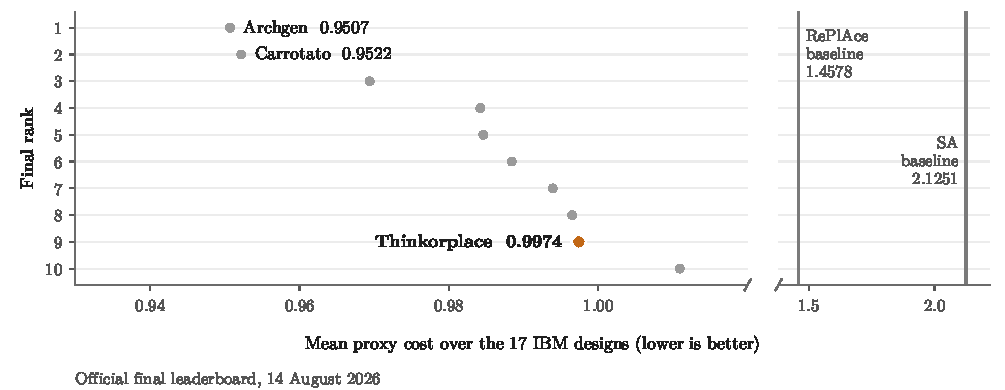
\includegraphics{figures/result_context.pdf}
\caption{The ranked entry in context (\official): mean proxy over the 17 IBM designs
for the top ten of the final leaderboard and the published RePlAce and
simulated-annealing (SA) baselines (broken axis; lower is better).}
\label{fig:result-context}
\end{figure}

\section{Introduction}\label{sec:intro}

A chip design starts as a \emph{netlist}: a list of components, each with connection
points called \emph{pins}, and of \emph{nets}, the groups of pins that must be wired
together. The largest components are \emph{macros}, pre-designed blocks such as
memories, each a fixed rectangle far larger than a logic gate. Around them sit many
thousands of small \emph{standard cells}; the benchmarks group these into \emph{soft
clusters}, movable blobs that may overlap one another. \emph{Macro placement}
chooses where the macros, and in this competition the soft clusters too, should go
(\cref{fig:placement}). A good placement keeps connected blocks close, so wires are
short, without crowding them so much that the wires cannot all be routed between
them.

\begin{figure}[tbp]
\centering
\sbox{\sidefigbox}{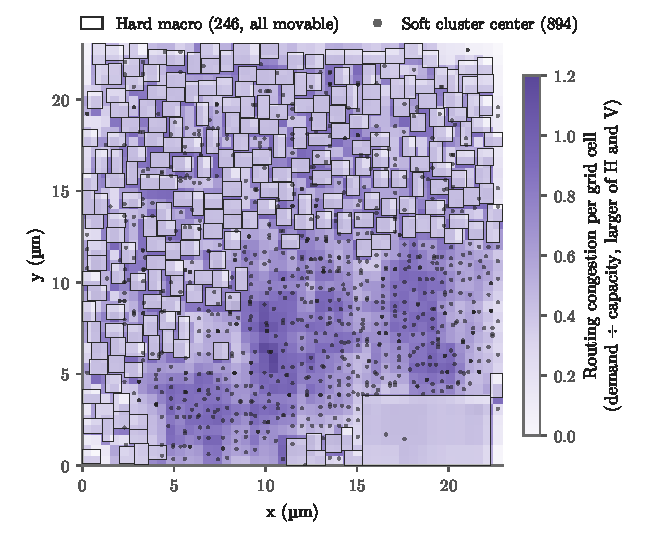
\includegraphics{figures/placement_ibm01.pdf}}%
\begin{minipage}[c]{\wd\sidefigbox}\usebox{\sidefigbox}\end{minipage}\hfill
\begin{minipage}[c]{\dimexpr\linewidth-\wd\sidefigbox-1.2em\relax}
\captionsetup{justification=raggedright,singlelinecheck=false}
\caption{What a placement looks like: IBM01, the smallest design by canvas area and
net count, with 246 hard macros (outlined) and 894 soft-cluster centers on a
$22.95\times23.04\,\mu$m canvas, over the evaluator's routing congestion per grid
cell (darker is more congested). The placement comes from a research run of our
earlier v1 pipeline (\cref{sec:scored}), proxy 0.84528, rescored for this report
(\measurement); the judged entry's coordinates were not saved.}
\label{fig:placement}
\end{minipage}
\end{figure}

The Partcl/HRT Macro Placement Challenge 2026 \citep{challenge2026} posed this
problem on 17 public designs from the ICCAD04 IBM suite
\citep{adya2004unification}, each with 178--786 hard macros and 894--1,985 soft
clusters. Entries were ranked by a \emph{proxy score}, a fast stand-in for the
quality of a fully routed chip: a weighted sum of wirelength, density and routing
congestion computed by an open evaluator \citep{macroplacement} that implements the
Circuit Training proxy \citep{mirhoseini2021graph}.
Lower is better. Any overlap between two hard macros disqualified an entry, and each
design had a one-hour limit.

Two tools pull in opposite directions. A smooth approximation of the score can be
minimized by gradient descent, moving thousands of coordinates together, but it is
only approximate; the exact score is reliable but has kinks and jumps, and judges one
move at a time. Our approach therefore separates proposing moves from accepting them:
a differentiable \emph{surrogate} of the score moves all blocks together, a
\emph{legalizer} moves overlapping hard macros to nearby free spots until none
overlap, and \emph{coordinate descent}, which tries moving one block along one axis
at a time, keeps a move only if the exact score decreases. The ranked configuration
was listed at about 12 minutes per design and placed ninth
(\cref{fig:result-context}). We contribute:
\begin{itemize}[leftmargin=1.6em,topsep=0.3em,itemsep=0.15em]
  \item \textbf{a two-stage placer} in which a smooth surrogate proposes and the
        exact score decides; it is most likely the ranked entry, 31.6\% below the
        published RePlAce baseline and 4.9\% above the winner (\official);
  \item \textbf{exact scoring at local cost}: rescoring only what a move changes
        takes 1.3--3.7\,ms per sampled move against 1.4--26.9\,s for full
        recomputation (\measurement), roughly $10^3$--$2\times10^4$ times faster, so
        a 600\,s search can try about $10^5$ candidate moves instead of at most a
        few hundred; on the sampled states, rounding error is about a million times
        too small to make an accepted move raise the true score;
  \item \textbf{a mathematical framing, from standard tools, that explains the
        design}: for $m$ pairs of blocks the legal region is up to $4^m$ convex
        pieces, which is why one-block moves stay near their starting arrangement
        and the smooth start matters; crowding terms are averages over the worst
        cells, which bounds how far one move can shift them; a Taylor bound says
        when a kick along negative curvature must help a smooth function; and a
        two-block counterexample shows why an optimal reassignment still needs an
        exact recheck;
  \item \textbf{lessons from development records} (\historical): congestion supplied
        84.5\% of our improvement, a pipeline six times faster also scored better,
        and kicks along computed negative-curvature directions helped about equally
        in every direction tried, so the record cannot credit the curvature.
\end{itemize}

\paragraph{How to read this report.} Pages 1--3 and the ``In brief'' boxes tell the
story; \cref{sec:limitations} collects every caveat; the appendices hold the exact
score, settings, proofs, audit, per-design records and a glossary. Each result
carries one evidence label: \official{} for the organizers' final leaderboard,
\historical{} for May 2026 development records (unmatched in hardware, budget and
concurrency, mostly without saved coordinates), and \measurement{} for
post-competition microbenchmarks and diagnostics.

\section{The problem as optimization}\label{sec:problem}

\inbrief{Each pair of hard blocks must sit left of, right of, above or below one
another, so with $m$ pairs the legal placements form a union of up to $4^m$ convex
pieces, and a search that moves one block at a time can leave its piece only where
two pieces touch. The score averages the most crowded grid cells and assigns pins to
cells, so it has kinks and jumps where gradients fail, and one exact evaluation takes
seconds.}

\subsection{Variables and constraints}\label{sec:geometry}\label{sec:geometry-analysis}

The canvas is the rectangle $[0,L_x]\times[0,L_y]$. Object $i$, a hard macro or a
soft cluster, has center $p_i=(x_i,y_i)$, width $w_i$ and height $h_i$; sizes and
orientations are fixed. A placement $p$ stacks all centers into one vector, of
2,156--5,536 coordinates on the IBM designs. Every object must lie inside the
canvas,
\begin{equation}
  \tfrac{w_i}{2}\le x_i\le L_x-\tfrac{w_i}{2},\qquad
  \tfrac{h_i}{2}\le y_i\le L_y-\tfrac{h_i}{2},
  \label{eq:containment}
\end{equation}
and fixed objects keep their positions (no IBM design has any). Soft clusters may
overlap anything, but two hard macros $i\neq j$ must be separated horizontally or
vertically: at least one of four linear inequalities must hold,
\begin{equation}
\Bigl(x_i+\tfrac{w_i}{2}\le x_j-\tfrac{w_j}{2}\Bigr)\lor
\Bigl(x_j+\tfrac{w_j}{2}\le x_i-\tfrac{w_i}{2}\Bigr)\lor
\Bigl(y_i+\tfrac{h_i}{2}\le y_j-\tfrac{h_j}{2}\Bigr)\lor
\Bigl(y_j+\tfrac{h_j}{2}\le y_i-\tfrac{h_i}{2}\Bigr).
\label{eq:disjunction}
\end{equation}
Touching edges are legal. Choosing one of the four options for every pair turns this
either-or rule into ordinary linear inequalities, which gives the structure below.
Let $\mathcal B$ be the set of placements that satisfy
\eqref{eq:containment} and the fixed positions, $\mathcal E$ the set of unordered
hard-macro pairs with $m=|\mathcal E|$, and $H_{e,b}$ the closed halfspace given by
branch $b\in\{1,2,3,4\}$ of \eqref{eq:disjunction} for pair $e$.

\begin{proposition}[Finite polyhedral decomposition]\label{prop:geometry}
The feasible set is a union of at most $4^m$ compact convex polyhedra:
\begin{equation}
 \mathcal F
 =\mathcal B\cap\bigcap_{e\in\mathcal E}\bigcup_{b=1}^4 H_{e,b}
 =\bigcup_{\sigma\in\{1,2,3,4\}^{\mathcal E}} P_\sigma,
 \qquad
 P_\sigma=\mathcal B\cap\bigcap_{e\in\mathcal E}H_{e,\sigma(e)}.
 \label{eq:polyhedral-union}
\end{equation}
The polyhedra may overlap or be empty.
\end{proposition}
\noindent Proof in Appendix~\ref{app:proofs}. Each piece $P_\sigma$ fixes, for every
pair, which side of the other each macro lies on (\cref{fig:feasible}); IBM01's 246
hard macros form $m=30{,}135$ pairs, so up to $4^{30{,}135}$ pieces. Inside a piece the constraints are linear and
convex, so continuous optimization works, but changing a pair's arrangement means
moving to another piece, which a path that never overlaps can do only where two
pieces touch. Along one coordinate, with the others fixed, the legal values form a
finite union of closed intervals (Appendix~\ref{app:proofs}): a one-coordinate
search sees gaps where other blocks stand in the way.

\subsection{The score}\label{sec:score}\label{sec:tail-analysis}

The competition proxy, introduced with Circuit Training \citep{mirhoseini2021graph}
and computed by the TILOS MacroPlacement evaluator \citep{macroplacement}, is
\begin{equation}
  \proxy(p)=W(p)+\tfrac12 D(p)+\tfrac12 C(p).
  \label{eq:canonical}
\end{equation}
Appendix~\ref{app:objective} gives every constant.

\paragraph{Wirelength.} The half-perimeter wirelength (HPWL) of a net $n$ is half
the perimeter of the smallest rectangle around its pins, a standard estimate of the
wire needed to connect them. With each pin $q$ at a fixed offset from its object's
center and net weights $\omega_n$,
\[
 \mathrm{HPWL}_n=\bigl(\max_{q\in n}x_q-\min_{q\in n}x_q\bigr)
 +\bigl(\max_{q\in n}y_q-\min_{q\in n}y_q\bigr),
 \qquad
 W=\frac{\sum_n\omega_n\,\mathrm{HPWL}_n}{(L_x+L_y)\sum_n\omega_n}.
\]

\paragraph{Tail averages.} Density and congestion use a grid of $G$ cells (810 to
2,255 per design). For $N$ cell values $z\in\mathbb R^N$, let $A_k(z)$ be the mean of
the $k$ largest: \emph{the average of the worst $k$ cells}. With $\rho_b$ the total
object area in cell $b$ divided by the cell area (it exceeds 1 where objects
overlap), $D=\tfrac12A_{\lfloor0.1G\rfloor}(\rho)$ with $N=G$, so the raw top-decile
mean enters $\proxy$ with weight $\tfrac14$. \emph{Routing congestion} compares
wiring demand with the routing tracks available: the evaluator maps each pin to the
grid cell that contains it, routes each net between those cells with simple L- and
T-shaped paths, divides each cell's horizontal and vertical demand by its capacity,
spreads it evenly over the cell and up to two neighbors on each side along one axis,
and adds a fixed allowance for macros covering the cell. With $u\in\mathbb R^{2G}$
the horizontal and vertical values, $C=A_{\lfloor0.05\cdot2G\rfloor}(u)$ with
$N=2G$, the mean of the worst 5\%.

\begin{lemma}[Tail representation and stability]\label{lem:tail}
For $z\in\mathbb R^N$, an integer $1\le k\le N$ and $(a)_+=\max\{a,0\}$,
\begin{equation}
 A_k(z)
 =\max_{\substack{0\le\beta_j\le1/k\\\sum_j\beta_j=1}}\beta^\top z
 =\min_{\theta\in\mathbb R}\Bigl\{\theta+
 \frac1k\sum_{j=1}^N(z_j-\theta)_+\Bigr\}.
 \label{eq:tail-representation}
\end{equation}
$A_k$ is convex and piecewise affine, and for any $\delta\in\mathbb R^N$,
\begin{equation}
 |A_k(z+\delta)-A_k(z)|
 \le\min\Bigl\{\|\delta\|_\infty,\
          \frac{\|\delta\|_2}{\sqrt{k}},\
          \frac{\|\delta\|_1}{k}\Bigr\}.
 \label{eq:tail-stability}
\end{equation}
\end{lemma}
\noindent The threshold form is the conditional value-at-risk formula
\citep{rockafellar2000cvar}; proof in Appendix~\ref{app:proofs}. For the solver, the
tails are convex in the cell values but kinked wherever the set of worst cells
changes, and they are not convex in block positions, because cell values depend on
positions nonlinearly. A move that changes the cells by $\delta$ moves a tail by at
most $\|\delta\|_1/k$, so a move that touches few cells shifts the crowding terms
little: the first sampled IBM01 move changed 12 of 1,845 cells and the density
component $D=\tfrac12A_k$ by 0.0025, within its bound $\tfrac12\|\delta\|_1/k=0.0153$
(\measurement). The same locality is what \cref{sec:cheap} exploits.

\subsection{Why it is hard}\label{sec:hard}

\begin{itemize}[leftmargin=1.4em,topsep=0.2em,itemsep=0.2em]
  \item \textbf{Nonconvex and disconnected:} good placements in different pieces can
        be separated by overlapping states that no legal path crosses.
  \item \textbf{Piecewise and discontinuous:} pin extremes, clamps and top-$k$
        selection leave kinks, and because the congestion estimate assigns pins to
        grid cells, the score jumps whenever a pin crosses a grid line; its routing
        part has zero gradient almost everywhere.
  \item \textbf{Expensive:} a full evaluation with the reference evaluator took
        1.4\,s on IBM01 and 27\,s on IBM10 (\measurement), so an hour buys about
        2,600 and 130 of them.
  \item \textbf{Large and conflicting:} thousands of coordinates interact through
        7,269--83,132 nets, and packing connected blocks shortens wires but narrows
        routing channels (\cref{fig:placement-tradeoff}); weighted congestion is
        about two-thirds of the score in every development record (\historical).
\end{itemize}

\begin{figure}[tbp]
\centering
\begin{subfigure}[b]{0.6\linewidth}
\centering
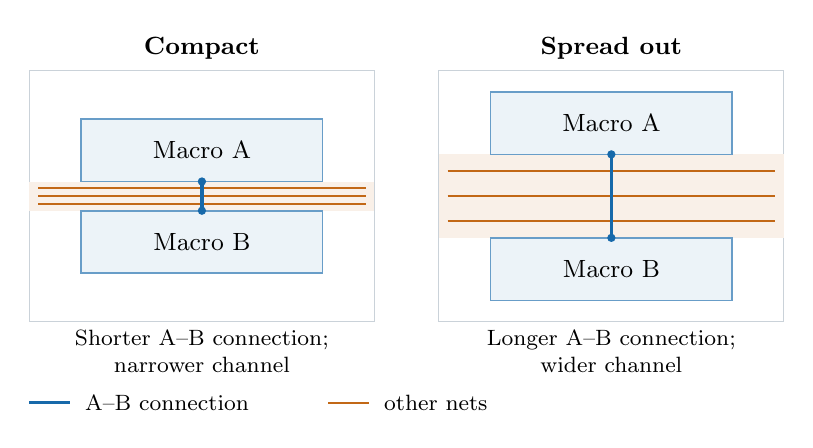
\begin{tikzpicture}[x=0.73cm,y=0.53cm,font=\small,
  block/.style={draw=blue!65,fill=blue!8,line width=0.6pt},
  route/.style={draw=orange,line width=0.7pt},
  connection/.style={draw=blue,line width=1.3pt}]
  \begin{scope}
    \node[font=\small\bfseries] at (3,6.55) {Compact};
    \draw[rulegray] (0,0) rectangle (6,6);
    \path[fill=orange!10] (0,2.65) rectangle (6,3.35);
    \draw[block] (0.9,3.35) rectangle (5.1,4.85);
    \draw[block] (0.9,1.15) rectangle (5.1,2.65);
    \node at (3,4.1) {Macro A};
    \node at (3,1.9) {Macro B};
    \foreach \y in {2.8,3.0,3.2} {\draw[route] (0.15,\y) -- (5.85,\y);}
    \draw[connection] (3,2.65) -- (3,3.35);
    \fill[blue] (3,2.65) circle (1.5pt);
    \fill[blue] (3,3.35) circle (1.5pt);
    \node[align=center,font=\footnotesize] at (3,-0.72)
      {Shorter A--B connection;\\narrower channel};
  \end{scope}
  \begin{scope}[xshift=5.2cm]
    \node[font=\small\bfseries] at (3,6.55) {Spread out};
    \draw[rulegray] (0,0) rectangle (6,6);
    \path[fill=orange!10] (0,2.0) rectangle (6,4.0);
    \draw[block] (0.9,4.0) rectangle (5.1,5.5);
    \draw[block] (0.9,0.5) rectangle (5.1,2.0);
    \node at (3,4.75) {Macro A};
    \node at (3,1.25) {Macro B};
    \foreach \y in {2.4,3.0,3.6} {\draw[route] (0.15,\y) -- (5.85,\y);}
    \draw[connection] (3,2.0) -- (3,4.0);
    \fill[blue] (3,2.0) circle (1.5pt);
    \fill[blue] (3,4.0) circle (1.5pt);
    \node[align=center,font=\footnotesize] at (3,-0.72)
      {Longer A--B connection;\\wider channel};
  \end{scope}
  \draw[connection] (0,-1.95) -- (0.7,-1.95);
  \node[anchor=west,font=\footnotesize] at (0.8,-1.95) {A--B connection};
  \draw[route] (5.2,-1.95) -- (5.9,-1.95);
  \node[anchor=west,font=\footnotesize] at (6.0,-1.95) {other nets};
\end{tikzpicture}
\caption{Why the terms compete (schematic).}
\label{fig:placement-tradeoff}
\end{subfigure}\hfill
\begin{subfigure}[b]{0.38\linewidth}
\centering
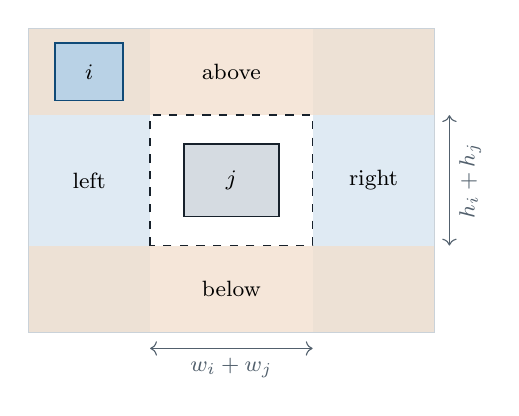
\begin{tikzpicture}[x=0.86cm,y=0.92cm,font=\footnotesize]
  \fill[blue!14] (0,0) rectangle (1.8,4.2);
  \fill[blue!14] (4.2,0) rectangle (6,4.2);
  \fill[orange!22,opacity=0.75] (0,3.0) rectangle (6,4.2);
  \fill[orange!22,opacity=0.75] (0,0) rectangle (6,1.2);
  \draw[rulegray] (0,0) rectangle (6,4.2);
  \draw[dashed,ink,line width=0.6pt,fill=white] (1.8,1.2) rectangle (4.2,3.0);
  \draw[ink,fill=rulegray!80,line width=0.6pt] (2.3,1.6) rectangle (3.7,2.6);
  \node at (3.0,2.1) {$j$};
  \draw[blue!70!black,fill=blue!30,line width=0.6pt] (0.4,3.2) rectangle (1.4,4.0);
  \node at (0.9,3.6) {$i$};
  \node at (0.9,2.1) {left};
  \node at (5.1,2.1) {right};
  \node at (3.0,3.6) {above};
  \node at (3.0,0.6) {below};
  \draw[<->,muted] (1.8,-0.22) -- node[below]{$w_i+w_j$} (4.2,-0.22);
  \draw[<->,muted] (6.22,1.2) -- node[below,rotate=90]{$h_i+h_j$} (6.22,3.0);
\end{tikzpicture}
\caption{Where $i$'s center may go ($j$ fixed).}
\label{fig:feasible}
\end{subfigure}
\caption{(a)~More separation leaves room for wires crossing between two blocks but
lengthens their connection (schematic; macro interiors obstruct routing). (b)~Each
branch of \eqref{eq:disjunction} confines $i$'s center to a halfplane left of, right
of, below or above $j$; their union, the plane minus the dashed box, is not convex,
and corners satisfy two branches ($i$ is drawn in the upper-left corner).}
\label{fig:problem-pictures}
\end{figure}

\section{Approach}\label{sec:approach}\label{sec:system}

\inbrief{A smooth surrogate moves all blocks together, a legalizer removes overlaps,
and coordinate descent keeps a change only if the exact score drops, at milliseconds
per check. Two add-on lanes for escaping stalls, kicks along negative-curvature
directions and optimal reassignment of blocks to slots, were committed on
21--22 May; we infer they were never scored.}

The surrogate proposes and the exact score accepts (\cref{fig:architecture}); this
section describes each stage, then what was scored.

\begin{figure}[tbp]
\centering
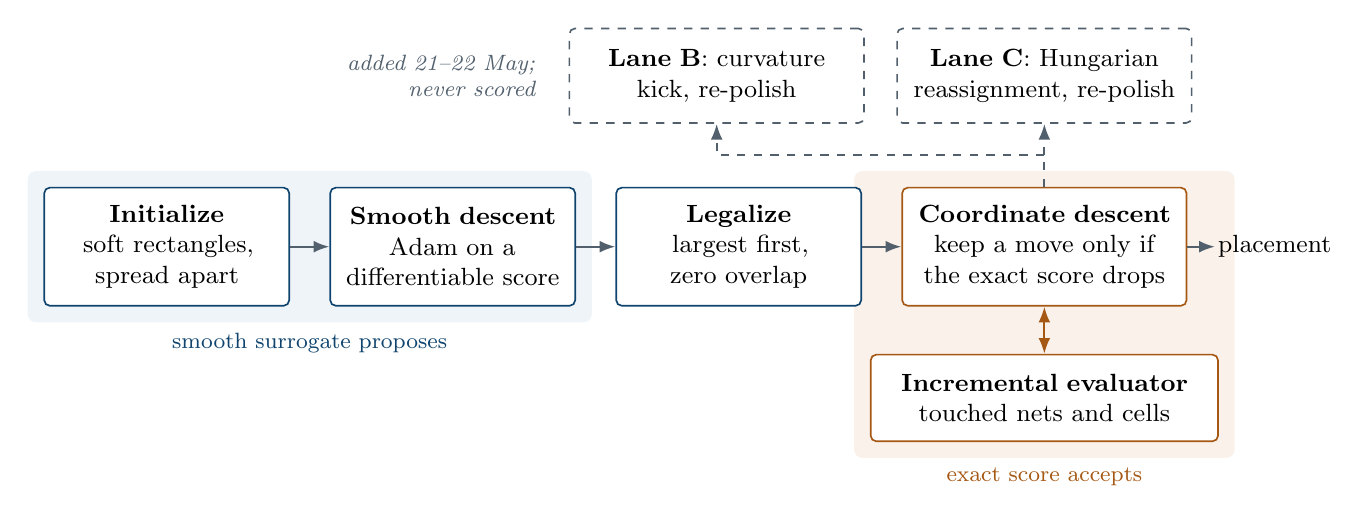
\begin{tikzpicture}[font=\small,
  stage/.style={draw=blue!65!black,fill=white,rounded corners=2pt,line width=0.6pt,
    text width=29mm,minimum height=15mm,align=center,inner sep=3pt},
  exact/.style={stage,draw=orange!85!black},
  ext/.style={draw=muted,dashed,fill=white,rounded corners=2pt,line width=0.6pt,
    text width=36mm,minimum height=12mm,align=center,inner sep=2pt},
  arr/.style={-{Latex[length=2mm]},thick,color=muted},
  darr/.style={-{Latex[length=2mm]},thick,dashed,color=muted}]
  \node[stage] (init) {\textbf{Initialize}\\soft rectangles,\\spread apart};
  \node[stage,right=5mm of init] (smooth) {\textbf{Smooth descent}\\Adam on a\\differentiable score};
  \node[stage,right=5mm of smooth] (legal) {\textbf{Legalize}\\largest first,\\zero overlap};
  \node[exact,right=5mm of legal,text width=34mm] (cd) {\textbf{Coordinate descent}\\keep a move only if\\the exact score drops};
  \node[right=3.5mm of cd,align=center,inner sep=1pt] (out) {placement};
  \node[exact,below=6mm of cd,text width=42mm,minimum height=11mm] (eval)
    {\textbf{Incremental evaluator}\\touched nets and cells};
  \draw[arr] (init) -- (smooth);
  \draw[arr] (smooth) -- (legal);
  \draw[arr] (legal) -- (cd);
  \draw[arr] (cd) -- (out);
  \draw[{Latex[length=2mm]}-{Latex[length=2mm]},thick,color=orange!85!black] (cd) -- (eval);
  \node[ext,above=8mm of cd] (lanec) {\textbf{Lane C}: Hungarian\\reassignment, re-polish};
  \node[ext,left=4mm of lanec] (laneb) {\textbf{Lane B}: curvature\\kick, re-polish};
  \coordinate (j) at ($(cd.north)+(0,4mm)$);
  \draw[dashed,thick,muted] (cd.north) -- (j);
  \draw[darr] (j) -| (laneb.south);
  \draw[darr] (j) -- (lanec.south);
  \node[left=3mm of laneb,align=right,font=\footnotesize\itshape,color=muted]
    {added 21--22 May;\\never scored};
  \begin{scope}[on background layer]
    \node[fit=(init)(smooth),fill=blue!7,rounded corners=3pt,inner sep=2mm,
      label={[font=\footnotesize,text=blue!65!black]below:smooth surrogate proposes}] {};
    \node[fit=(cd)(eval),fill=orange!9,rounded corners=3pt,inner sep=2mm,
      label={[font=\footnotesize,text=orange!85!black]below:exact score accepts}] {};
  \end{scope}
\end{tikzpicture}
\caption{Architecture. The ranked entry is inferred to have run the solid pipeline:
the smooth surrogate proposes (blue) and the exact, incrementally computed score
accepts (orange). Dashed lanes B and C were committed before the deadline but, by the
same inference, never scored; the predecessor v1 (\cref{sec:scored}) is not shown.}
\label{fig:architecture}
\end{figure}

\subsection{Make the exact score cheap}\label{sec:cheap}\label{sec:incremental-analysis}

The evaluator caches pin positions, net bounding boxes, cell densities, net routing
contributions and macro allowances. Moving object $i$ changes only its pins, its
nets, and the cells under its footprint and along those nets' routes, so the
evaluator subtracts old contributions, adds new ones, re-reads the tails, and can
revert. On 14 distinct moves from IBM01 and IBM10, repeated in two or three batches,
an update took 1.29--3.67\,ms against 1.40--26.87\,s for full recomputation with the
reference Python evaluator, excluding setup and overlap checks (\measurement):
roughly $10^3$--$2\times10^4$ times faster per sampled move. This is what makes
exact search affordable: a 600\,s pass can try about $10^5$ candidates instead of
22--430 with full recomputation. The ratio reflects both the local-update strategy
and a faster implementation, and re-selecting the top $k$ of $G$ cells still costs
time linear in the grid size. Floating-point updates need not cancel exactly, so the
incremental score $\widehat J$ can drift from $\proxy$; the largest relative
component discrepancy was $2.6\times10^{-15}$.

\begin{proposition}[Acceptance under bounded score error]\label{prop:acceptance}
Let $S_p$ and $S_q$ be the incremental states at candidate endpoints $p$ and $q$,
and suppose $|\widehat J(S_p)-\proxy(p)|\le\epsilon$ and
$|\widehat J(S_q)-\proxy(q)|\le\epsilon$. If $\widehat J(S_q)\le\widehat J(S_p)-\tau$,
then
\begin{equation}
 \proxy(q)-\proxy(p)\le-\tau+2\epsilon.
 \label{eq:acceptance-error}
\end{equation}
In particular, $\tau>2\epsilon$ guarantees a strict decrease of the true score.
\end{proposition}
\noindent Proof in Appendix~\ref{app:proofs}. Coordinate descent uses
$\tau=10^{-9}$, and the largest absolute proxy discrepancy over 36 sampled endpoints
was $\epsilon=4.44\times10^{-16}$, so $\tau/2\epsilon\approx1.1\times10^6$
(\measurement): on those states the error would have to be a million times larger
before an accepted move could raise the true score. This is a sampled margin, not a
uniform bound. The sample exercises the single-move path; coordinate descent scores
candidates through a batched float64 path that was not sampled separately, and
rescoring 34 saved endpoints reproduced their recorded scores only to about
$10^{-7}$.

\subsection{Smooth proposals}\label{sec:smooth}

The smooth stage minimizes a differentiable surrogate of \eqref{eq:canonical},
\begin{equation}
\surrogate(p)=\widetilde W_\gamma(p)+\tfrac12\widetilde D(p)+\tfrac12\widetilde C(p)
 +\lambda_t P_{\mathrm{ov}}(p)+\mu P_{\mathrm{out}}(p),
\label{eq:surrogate}
\end{equation}
which replaces each kink of the score by a smooth approximation and adds penalties
for hard-macro overlap ($P_{\mathrm{ov}}$) and for leaving the canvas
($P_{\mathrm{out}}$). It starts from a soft-rectangle initializer that spreads the
hard macros apart by gradient steps; soft clusters start from the benchmark's input
coordinates, which derive from a RePlAce placement (Appendix~\ref{app:objective}).

\paragraph{Wirelength: a smooth maximum.} HPWL uses $\max$ and $\min$, which have no
gradient where the extreme pin changes. Log-sum-exp replaces the maximum by a smooth
one \citep{naylor2001lse}: for values $x_1,\dots,x_r$ and smoothing length
$\gamma>0$,
\begin{equation}
 \max_j x_j\ \le\ \gamma\log\sum_{j=1}^r e^{x_j/\gamma}\ \le\ \max_j x_j+\gamma\log r,
 \label{eq:lse}
\end{equation}
because the sum contains $e^{\max_j x_j/\gamma}$ and is at most $r$ times it; as
$\gamma\to0$ it converges to the true maximum, and $\min_j x_j=-\max_j(-x_j)$. A
large $\gamma$ is smooth but biased, a small one accurate but stiff, so we anneal
$\gamma$ from $5\times10^{-3}$ to $5\times10^{-5}$ of the canvas scale.

\paragraph{Density: Gaussian smearing.} A rectangle's share of a cell changes at a
rate that jumps when its edge crosses the cell boundary. We instead spread each
object $i$, hard macro or soft cluster, of area $A_i=w_ih_i$, as a separable Gaussian
with spreads $\sigma_{xi}=\max(w_i/2,\Delta_x/2)$ and
$\sigma_{yi}=\max(h_i/2,\Delta_y/2)$, where $\Delta_x\times\Delta_y$ is the cell size.
With $\Phi$ the standard normal distribution function, its mass in cell
$b=[x_b^-,x_b^+]\times[y_b^-,y_b^+]$ is
\begin{equation}
m_{ib}=A_i
\Bigl[\Phi\Bigl(\tfrac{x_b^+-x_i}{\sigma_{xi}}\Bigr)-
      \Phi\Bigl(\tfrac{x_b^--x_i}{\sigma_{xi}}\Bigr)\Bigr]
\Bigl[\Phi\Bigl(\tfrac{y_b^+-y_i}{\sigma_{yi}}\Bigr)-
      \Phi\Bigl(\tfrac{y_b^--y_i}{\sigma_{yi}}\Bigr)\Bigr],
\label{eq:gaussian-density}
\end{equation}
a smooth function of position; $\widetilde D$ applies the top-decile rule to the cell
densities $\tilde\rho_b=\sum_im_{ib}/(\Delta_x\Delta_y)$. Top-$k$ selection and
canvas clamps keep some kinks. This smoother density is the surrogate change the
development records credit (\cref{tab:development}, row~9).

\paragraph{Congestion: a routing trace.} RUDY spreads a net's demand uniformly over
its bounding box \citep{spindler2007rudy}; the evaluator routes along rows and
columns, and our surrogate follows it. Each source--sink pin pair adds a horizontal
stripe along the source's row and a vertical stripe along the sink's column, with
soft (sigmoid) cell membership so the stripes move smoothly with the pins; the macro
allowance, smoothing and top-5\% tail follow the evaluator.

\paragraph{Overlap, optimizer and legalization.} $P_{\mathrm{ov}}$ sums hard-macro
penetration areas, with a weight $\lambda_t$ that rises over the first 70\% of the
steps, so the surrogate first finds an arrangement and then pushes blocks apart;
$P_{\mathrm{out}}$ penalizes positions outside the canvas, with weight $\mu$. Adam, a
standard gradient optimizer \citep{kingma2015adam}, takes 500 steps.
\emph{Legalization} then turns the almost-legal result into one with zero overlap
while moving blocks as little as possible: in order of decreasing area, each hard
macro keeps its position if free or moves to the first free spot, in a fixed scan
order, on the nearest ring that has one; a push-apart pass and, if needed, a retry
with a stronger overlap weight remove the rest.

\subsection{Exact local search}\label{sec:cd}

Coordinate descent \citep{wright2015coordinate} visits every movable object, hard
macros and soft clusters alike, in random order. For each coordinate it takes the
legal interval around the current position, bounded by the nearest blocking macros
(within one of the intervals of \cref{sec:geometry}), and scores at most ten
candidates there in one batched incremental call: the ends and midpoint, the current
position, the nearest grid-line crossings, and targets suggested by the object's
nets. The best is kept if it lowers the score by more than $\tau=10^{-9}$. A pass
stops at its time cap or, after half of it, once five consecutive sweeps each gain
less than 0.001. Every accepted step lowers the incremental score and, by
\cref{prop:acceptance} with the sampled margin, the exact score of the internal
float64 state. The price is reach: a one-coordinate move changes a pair's
arrangement only at a point of contact, so coordinate descent stays near the
arrangement it starts from, and the smooth start matters (\cref{sec:simpler}).

\subsection{Escaping plateaus}\label{sec:escape}\label{sec:curvature}\label{sec:assignment-analysis}

When coordinate descent stalls, further gains need many blocks to move at once. We
tried two such \emph{proposals}; every candidate is legalized, re-polished by
coordinate descent and kept only if the exact score drops.

\paragraph{(a) Negative curvature.} Near a placement $p$, a smooth function $f$
behaves like its second-order Taylor expansion along a unit direction $v$:
\begin{equation}
 f(p+tv)\approx f(p)+t\,\nabla f(p)^\top v+\tfrac12t^2\,v^\top \mathbf H v,
 \qquad \mathbf H=\nabla^2 f(p).
 \label{eq:taylor}
\end{equation}
Where small moves stop helping, the gradient term is small; if the curvature
$v^\top\mathbf Hv$ is negative, the surface bends down along $v$, and a step of
moderate length lowers $f$. The most negative curvature is the smallest eigenvalue
of $\mathbf H$, a matrix with about 5.2 million entries on IBM01. We never build
it: automatic differentiation gives a Hessian-vector product $\mathbf Hv$ at a small
multiple of the cost of a gradient \citep{pearlmutter1994hvp}, and the Lanczos
method \citep{lehoucq1998arpack} turns a few dozen such products into a small
subspace whose extreme eigenvalues approximate those of $\mathbf H$. That finds the
most negative curvature direction without ever building the matrix.

\begin{proposition}[Signed curvature decrease]\label{prop:curvature}
Let $f$ be twice continuously differentiable on an open set $U$ containing $p$, and
let $v$ be a unit vector with $v^\top\nabla^2 f(p)v\le-\eta<0$. Choose
$s\in\{-1,1\}$ with $s\,\nabla f(p)^\top v\le0$. Fix $t>0$, and suppose the segment
$\{p+usv:0\le u\le t\}$ lies in $U$ and the Hessian is $L$-Lipschitz on it
(Euclidean norm for vectors, induced norm for matrices). Then
\begin{equation}
 f(p+tsv)-f(p)\le-\frac{\eta}{2}t^2+\frac{L}{6}t^3.
 \label{eq:curvature-taylor}
\end{equation}
For $L>0$ and $0<t\le3\eta/(2L)$ this is at most $-\eta t^2/4$; for $L=0$ the bound is
$-\eta t^2/2$ throughout the segment.
\end{proposition}
\noindent Proof in Appendix~\ref{app:proofs}. In words: step along a direction of
negative curvature, with the sign chosen so the slope does not hurt, and $f$ falls by
at least $\eta t^2/4$ as long as the step is too short for the curvature to change
much; the gradient need not vanish. The guarantee does not carry over to the kicks we
ran. Legalization moves the endpoint after the step. The function $f$ was not the
exact score or the surrogate of \cref{sec:smooth} but an older surrogate kept for the
kicks, whose density and congestion terms multiply horizontal by vertical overlap
lengths; such products have negative-curvature directions built in, so finding one
says nothing by itself about the true score. And at the diagnosed IBM01 endpoint that
surrogate changes branch within $10^{-7}\,\mu$m, while the steps are
0.3--3\,$\mu$m long, so the Lipschitz hypothesis fails at the step length used.

\paragraph{(b) Assignment.} Some gains need two blocks to trade places, which
coordinate descent cannot do without passing through an overlap. The assignment move
draws $K=50$ macros at random from the 150 with the highest connectivity scores,
takes 100 candidate slots that include the macros' current centers, so staying put is
always possible, and scores each single move against a frozen background,
$\Delta_{ij}=\proxy(p^{i\leftarrow j})-\proxy(p^0)$, where $p^{i\leftarrow j}$ moves
only macro $i$ to slot $j$. The Hungarian method \citep{kuhn1955hungarian} then
solves
\begin{equation}
 \min_z\sum_{i,j}\Delta_{ij}z_{ij}
 \quad\text{subject to}\quad
 \sum_jz_{ij}=1,\quad\sum_iz_{ij}\le1,\quad z_{ij}\in\{0,1\}
 \label{eq:assignment-model}
\end{equation}
exactly, in time cubic in $K$. The moves are applied in order of predicted gain,
skipping any that would overlap, and the batch is kept only if the incremental score
falls by more than $10^{-7}$ (a sampled margin of $1.1\times10^8$ by
\cref{prop:acceptance}; \measurement).

\begin{figure}[tbp]
\centering
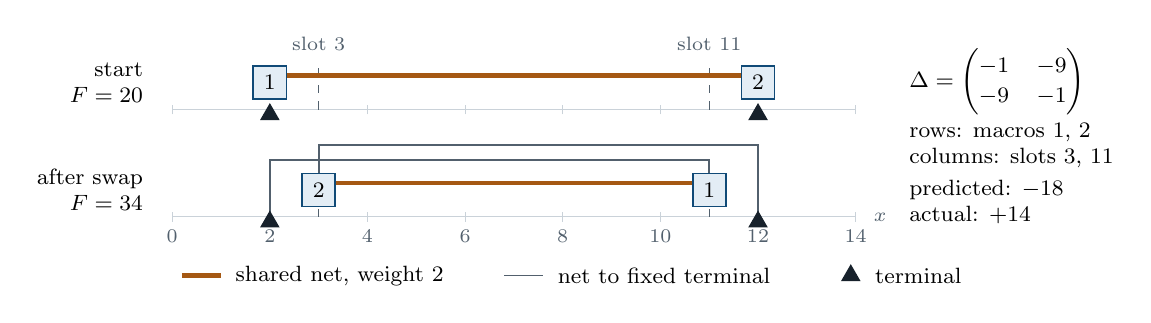
\begin{tikzpicture}[x=0.62cm,y=0.62cm,font=\footnotesize,
  mac/.style={draw=blue!70!black,fill=blue!12,line width=0.6pt,minimum size=4.2mm,inner sep=0pt},
  term/.style={draw=ink,fill=ink,regular polygon,regular polygon sides=3,minimum size=2.6mm,inner sep=0pt},
  shared/.style={draw=orange!85!black,line width=1.6pt},
  tether/.style={draw=muted,line width=0.7pt}]
  \foreach \yy in {2.2,0} {
    \draw[rulegray] (0,\yy-0.55) -- (14,\yy-0.55);
    \foreach \t in {0,2,...,14} {\draw[rulegray] (\t,\yy-0.65) -- (\t,\yy-0.45);}
    \foreach \s in {3,11} {\draw[dashed,muted] (\s,\yy-0.55) -- (\s,\yy+0.45);}
  }
  \foreach \t in {0,2,...,14} {\node[muted,font=\scriptsize] at (\t,-0.95) {\t};}
  \node[muted,font=\scriptsize] at (14.5,-0.55) {$x$};
  \node[anchor=east,align=right] at (-0.4,2.2) {start\\$F=20$};
  \draw[shared] (2,2.35) -- (12,2.35);
  \node[mac] at (2,2.2) {1}; \node[mac] at (12,2.2) {2};
  \node[term] at (2,1.55) {}; \node[term] at (12,1.55) {};
  \node[anchor=east,align=right] at (-0.4,0) {after swap\\$F=34$};
  \draw[shared] (3,0.15) -- (11,0.15);
  \draw[tether] (11,0.3) |- (2,0.62) -- (2,-0.5);
  \draw[tether] (3,0.3) |- (12,0.92) -- (12,-0.5);
  \node[mac] at (11,0) {1}; \node[mac] at (3,0) {2};
  \node[term] at (2,-0.65) {}; \node[term] at (12,-0.65) {};
  \node[muted,font=\scriptsize] at (3,3.0) {slot $3$};
  \node[muted,font=\scriptsize] at (11,3.0) {slot $11$};
  \node[anchor=west,align=left] at (14.9,1.1)
    {$\Delta=\begin{pmatrix}-1&-9\\-9&-1\end{pmatrix}$\\[2pt]
     rows: macros 1, 2\\ columns: slots 3, 11\\[2pt]
     predicted: $-18$\\ actual: $+14$};
  \draw[shared] (0.2,-1.75) -- (1.0,-1.75);
  \node[anchor=west] at (1.1,-1.75) {shared net, weight 2};
  \draw[tether] (6.8,-1.75) -- (7.6,-1.75);
  \node[anchor=west] at (7.7,-1.75) {net to fixed terminal};
  \node[term] at (13.9,-1.75) {};
  \node[anchor=west] at (14.2,-1.75) {terminal};
\end{tikzpicture}
\caption{An optimal assignment can make things worse: each of the two crossing moves
saves 9 on its own, so the matrix $\Delta$ predicts $-18$ for the swap, but done
together the moves cross and wirelength rises from 20 to 34.}
\label{fig:assignment}
\end{figure}

The matrix sees each move alone, but moves interact (\cref{fig:assignment}). Two
macros at $x_1=2$ and $x_2=12$ share a weight-2 net, and each has a unit-weight net to
a fixed terminal at its start, so up to normalization their wirelength is
\begin{equation}
 F(x_1,x_2)=2|x_1-x_2|+|x_1-2|+|x_2-12|.
 \label{eq:assignment-example}
\end{equation}
For slots 3 and 11, the Hungarian method picks $(x_1,x_2)=(11,3)$ with predicted
change $-18$, yet $F(2,12)=20$ and $F(11,3)=34$: the real change is $+14$, an
interaction residual of $+32$, with every placement legal for macros narrower than
one unit. Single-move gains ignore shared nets and, in the full score, the coupling
of all moves through the top-$k$ tails. Independent-set matching avoids the
wirelength part of this error by matching only cells that share no nets
\citep{chen2008ntuplace3}; our lane picks connected macros on purpose and relies on
the exact recheck.

\subsection{What was scored and what was added later}\label{sec:scored}

\paragraph{The ranked pipeline.} We infer that the entry verified at 0.9974,
resubmitted on 20 May, ran the solid pipeline of \cref{fig:architecture}, which we
call the \emph{single pipeline}, with a 720\,s budget, up to 600\,s of it for
coordinate descent. We did not record which commit the organizers ran; we infer the
configuration from the listed 12 minutes per design and the resubmission date
(Appendix~\ref{app:records}). Its smooth descent runs in single precision on a CUDA
GPU, an Apple GPU or the CPU, whichever is available, so the trajectory depends on
the device, and we have no record of the device used for the judged run.

\paragraph{Lanes B and C.} On 21--22 May, before the deadline, we committed a
three-lane system: Lane A is the same pipeline with a longer budget (2,700\,s, up to
900\,s of coordinate descent), Lanes B and C add the curvature kicks and assignment
batches, and the lowest exact score with zero overlaps wins. By the same inference it
was never scored, so 0.9974 says nothing about it.

\paragraph{The predecessor, v1.} Our 13 May entry, v1, polished two initial
placements serially with coordinate descent, large-neighborhood search and simulated
annealing \citep{kirkpatrick1983sa}, then ran a curvature cascade; a 17 May run of a
later v1 variant took about 53 minutes per design.

\section{Results}\label{sec:results}

\inbrief{Ninth on the final leaderboard at a verified mean proxy of 0.9974, 31.6\%
below RePlAce and 4.9\% above the winner, in a listed 12 minutes per design. Most of our
improvement came from lower congestion, and in the development records the fastest
pipeline also scored best.}

\subsection{Competition result}\label{sec:competition}

Our entry ranked ninth on the final leaderboard (verified mean proxy 0.9974; the
organizers report 132 verified eligible submissions), with zero overlaps and
per-design scores from 0.7829 to 1.2602 (\cref{tab:competition,fig:result-context};
\official). That is 31.6\% below the published RePlAce baseline
\citep{cheng2025updated} and 4.9\% above the winner; ranks four to nine lie within
1.4\% of one another. The listed 12 minutes per design is a fifth of the allowed
hour; among top-ten entries that list a runtime, only Vibe (516\,s) lists a shorter
one, on its own hardware. Before the 20 May resubmission, the leaderboard listed our
13 May entry (v1) at 1.0771; that earlier figure is not a verified result.

\begin{table}[htbp]
\centering
\footnotesize
\caption{Official, final leaderboard (14 August 2026). Mean proxy cost over the 17 IBM designs; lower is better. The organizers report 132 verified eligible submissions. Runtimes are as listed by each entrant on its own hardware; the last column is the change relative to the RePlAce mean.}
\label{tab:competition}
\begin{tabular}{clrrr}
\toprule
Rank & Entry & Mean proxy & Listed runtime & vs RePlAce \\
\midrule
1 & Archgen & 0.9507 & --- & $-34.8\%$ \\
2 & Carrotato & 0.9522 & $\sim$12.4\,min per design & $-34.7\%$ \\
\textbf{\boldmath 9} & \textbf{\boldmath Thinkorplace} & \textbf{\boldmath 0.9974} & \textbf{\boldmath 12\,min per design} & \textbf{\boldmath $-31.6\%$} \\
--- & RePlAce baseline & 1.4578 & --- & --- \\
--- & SA baseline & 2.1251 & --- & $+45.8\%$ \\
\bottomrule
\end{tabular}
\end{table}


\subsection{Where the gain came from}\label{sec:gain}

Three development records cover all 17 designs (\historical); the rest of this
section names them by their mean proxy. The \emph{v1 record} (1.05750) is a 17 May
run of a later variant of the serial v1 pipeline, not the 13 May entry. The
\emph{early single-pipeline record} (1.00835) is a 20 May run of an early version of
the single pipeline. The \emph{0.98199 record} is a 20 May run of the single-pipeline
version from which the ranked entry descends. They differ in code, hardware, budget
and concurrency, so they trace a trajectory rather than isolate causes. All three
beat both published baselines on every design, by 14--46\% against RePlAce
(Appendix~\ref{app:records}).

From the v1 record to the 0.98199 record the mean fell by 7.14\%, and
16 of 17 designs improved. The decrease of 0.07551 splits into 0.00294 from
wirelength, 0.00878 from weighted density and 0.06379 from weighted congestion, so
congestion supplied 84.5\% of the gain (\cref{fig:components}). That is where the
score lives: weighted congestion is 64.8--66.2\% of the mean proxy in each record.
The one regression, IBM02, shows the tradeoff of \cref{fig:placement-tradeoff}:
density fell, but wirelength and congestion rose (total 1.00659 to 1.01265). The
decomposition says which terms moved, not which code change moved them; the smooth
stage gained Gaussian density and the routing trace over the same period, and no
controlled ablation separates them.

\begin{figure}[tbp]
\centering
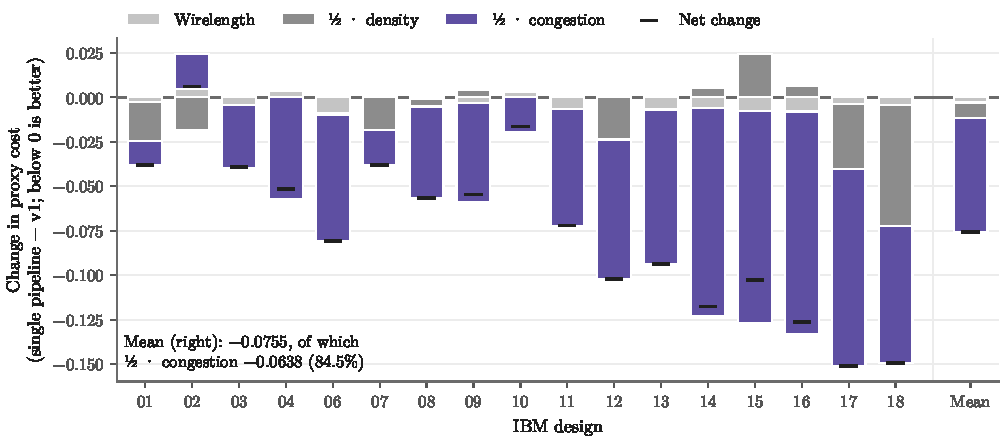
\includegraphics{figures/component_deltas.pdf}
\caption{Change in each weighted score component per design, from the v1 record to the
0.98199 record (20 May, single pipeline; \historical); bars below zero are
improvements, and congestion supplies 84.5\% of the mean decrease. The records are
unmatched in hardware, budget and concurrency.}
\label{fig:components}
\end{figure}

\subsection{A simpler, faster pipeline scored better}\label{sec:simpler}

The v1 record spent 3,192\,s per design on two initializers, three kinds of local
search and a curvature cascade; the early single-pipeline record spent 697\,s; and
the 0.98199 record spent 524\,s, a sixth of v1's time, and scored 7.1\% lower
(\historical). The ranked configuration descends from that pipeline; its official
score and this \historical{} record ran on different hardware with different settings
and are not compared here.

The geometry of \cref{sec:problem} suggests why: exact local search stays near the
arrangement it starts from (\cref{sec:cd}), so more of it mostly refines that
arrangement, while a better smooth start changes the arrangement itself. Only a
matched-compute comparison can test this reading.

\section{What worked and what did not}\label{sec:lessons}

\inbrief{Of 141 written hypotheses, 39 were explicitly falsified by pre-set kill
gates. Making the smooth model smoother helped; making it more accurate did not.
Curvature kicks helped about equally along every direction tried, so the record
cannot credit the curvature. A post-competition audit found ten defects; none is
known to have affected the judged entry.}

We ran development as written hypotheses, each with a kill gate (a pre-set threshold
for abandoning the idea) and a recorded outcome: 141 experiments, 39 explicitly
falsified (\historical). \Cref{tab:development} summarizes ten; they are single,
uncontrolled runs, so they show which ideas we kept and why rather than measure
effect sizes. Kill gates and cross-design checks caught a bug (row~3) and a move
that hurt industrial-style designs (row~5). Three lessons recur.

\begin{table}[htbp]
\centering
\footnotesize
\caption{What we tried during development (\historical). Each row summarizes single-run development records from April--May 2026. The runs are uncontrolled: hardware, time budget and concurrency varied, and most comparisons are against a separate reference run. Scores are proxy scores; lower is better. Row 1 gives the September re-measurement (\measurement) in place of the May figure. Verdict records the development decision at the time: \emph{kept}, adopted into a later pipeline; \emph{dropped}, abandoned after a negative result. Appendix~\ref{app:glossary} maps each numbered row to its record.}
\label{tab:development}
\begin{tabularx}{\linewidth}{@{}>{\raggedright\arraybackslash\hsize=0.9\hsize}X>{\raggedright\arraybackslash\hsize=1.1\hsize}Xl@{}}
\toprule
Idea (plain words) & What happened & Verdict \\
\midrule
1.~Rescore only what a one-block move changes, instead of recomputing the whole score & September re-measurement on two designs: 1.3--3.7 ms per move versus 1.4--26.9 s for a full rescore; largest relative difference $2.6\times10^{-15}$. & kept \\
\addlinespace[2pt]
2.~Move one block at a time along one axis to its best legal position; stop when gains level off rather than at a fixed time & Mean over 17 designs 1.1055, versus 1.1193 with a fixed 600 s stop, using 69\% more total time; hard designs gained 1.7--3.6\%, and all 17 stopped before the one-hour cap. & kept \\
\addlinespace[2pt]
3.~After local search stalls, accept some uphill moves at random (simulated annealing) & The first version was worse on 4 of 4 designs (by 5.7\% on average) because it returned its last state rather than its best. Fixed, it gained 0.63\% and became one stage of the earlier serial pipeline. & kept \\
\addlinespace[2pt]
4.~After local search converges, take GPU gradient steps on a smooth approximation of the score to find a better nearby arrangement & 0 of 350 attempts accepted on 4 designs at full budgets; a 2.16\% gain seen with shortened budgets did not reappear. & dropped \\
\addlinespace[2pt]
5.~Choose which blocks to remove and re-place by how much they add to routing congestion & Lower on 2 of 4 IBM designs (by 1.12\% and 0.15\%), but 1.45\% worse on four open industrial-style designs (5.14\% on one) and 0.39\% worse over all 17 IBM designs. & dropped \\
\addlinespace[2pt]
6.~Blend two good but different placements by moving every block partway along a straight line between them & On 2 designs, none of the 9 intermediate blends could be made overlap-free by the 50-iteration repair step; before repair, blends scored up to 61\% worse. & dropped \\
\addlinespace[2pt]
7.~Drive a mature open-source placer's optimizer (DREAMPlace) with the challenge score as its objective & On IBM01, 0.918 after repair and local search versus 0.852 for the existing pipeline (7.7\% worse); the optimizer left 118 overlaps for repair to fix. & dropped \\
\addlinespace[2pt]
8.~Make the smooth routing-congestion model agree more closely with the official scorer & On IBM17 the model's error fell from 14.4\% to 8.0\%, yet the final score was 0.98\% worse; a separate bug fix that also reduced the error changed it by 0.12\%, within noise. & dropped \\
\addlinespace[2pt]
9.~Spread each block's area as a smooth bell-shaped (Gaussian) blur when estimating crowding, so the gradient changes smoothly & Lower on 4 of 4 crowded designs (by 2.71\% on average) than the same pipeline with grid density. A later 17-design run averaged 0.98199, versus 1.05750 for the earlier serial pipeline, lower on 16 of 17. & kept \\
\addlinespace[2pt]
10.~Jointly reassign up to 50 highly connected blocks to candidate slots with an optimal matching (the Hungarian method), then rerun local search & Lower in 5 of 5 single-design trials (0.35--1.25\% against separate reference runs); part of the gain may come from the extra local-search pass. It went into an optional lane that is inferred never to have been scored. & kept \\
\bottomrule
\end{tabularx}
\end{table}


\paragraph{A smoother surrogate helped; a more faithful one did not.} Closer
agreement with the evaluator did not improve final scores (\historical): a
congestion model whose
IBM17 error fell from 14.4\% to 8.0\% left the final score 0.98\% worse (row~8;
within single-design run-to-run spread), and an earlier smooth score that ranked
saved placements well (Spearman 0.929) led descent from a good IBM01 placement to a
result 81\% worse after repair. Gradient polish did not improve converged placements
(rows~4 and~7); the change that helped, Gaussian density (row~9), made the surface
smoother, and its fidelity was not measured.

\paragraph{Good placements can be separated by illegal states.} Straight-line blends
between two good placements were never legal (0 of 9 on two designs; row~6),
consistent with \cref{prop:geometry}, which allows but does not require such gaps.

\paragraph{Curvature kicks helped, but the record cannot credit the curvature.} The
most elaborate idea has the clearest record (\cref{fig:curvature}; \historical). In
v1 research runs without the one-hour cap, a first curvature stage (up to 4,007\,s
per design) lowered the mean \emph{plateau} score, the better of v1's two branches
before any kick, from 1.08128 to 1.06760, and a cascade of further stages (up to
3,454\,s) reached 1.06119. Every design improved, but no design could have gotten
worse: a stage keeps its input unless a candidate scores lower. The informative
evidence is which kicks worked, and success barely depends on the eigenvector or the
step length. Of 204 first-stage attempts (12 on each design), 201 could be legalized
and 190 ended below the plateau with zero overlap: 94 of 102 along the first
eigenvector, 96 of 102 along the second, and 64, 65 and 61 of 68 at total
displacement norms of 0.3, 1 and 3\,$\mu$m summed over all blocks. Generic
perturb-and-repolish, or the extra polish alone, would produce this pattern; the
missing experiments are a random-direction control and a zero-step (polish-only)
control of equal cost.

\begin{figure}[tbp]
\centering
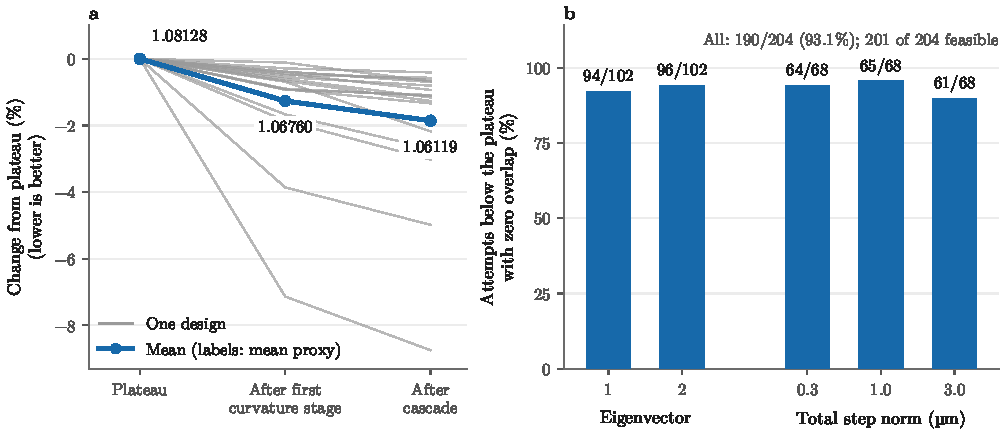
\includegraphics{figures/curvature_attempts.pdf}
\caption{Curvature kicks (perturb along a computed negative-curvature direction, then
legalize and re-polish) in v1 research runs without the one-hour cap (\historical):
(a)~score change relative to the plateau, the best v1 result before any kick, per
design and on average; (b)~share of first-stage attempts ending below the plateau
with zero overlap, by eigenvector and step length. Success is nearly the same in
every group, as generic perturb-and-repolish or the extra polish alone would also
produce.}
\label{fig:curvature}
\end{figure}

The curvature itself is doubtful. At one saved IBM01 placement, automatic
differentiation reports a negative curvature of $-0.442458$, but that number
describes only the smooth branch of the surrogate the point happens to sit on.
Density and congestion branch boundaries lie within $10^{-7}\,\mu$m, so a direct
finite-difference check sees jumps in the gradient instead; on the smooth wirelength
term the two agree to about $4\times10^{-9}$. The surrogate has no true second
derivative there: its eigenvectors are reasonable candidate directions, not
measurements of a bend in the score (\measurement; Appendix~\ref{app:curvature}).

\paragraph{Assignment.} Hungarian reassignment lowered the score in all 5
single-design trials (0.35--1.25\%; row~10), partly perhaps through its extra polish,
and went into Lane~C (\cref{sec:scored}).

\paragraph{Post-competition audit.} A September audit of the competition code found
ten defects, all since repaired (Appendix~\ref{app:verification}). Most were in
parts that were never scored, such as the three-lane supervisor, which waited
without a deadline once its budget had passed and saved lane results only on normal
completion, or in input parsing for hierarchical designs, which the flat IBM designs
never exercise; on all 17 IBM designs the repaired parsing yields identical inputs
(\measurement). Two could touch the single pipeline and cannot be excluded, because
no judged coordinates survive: float32 export can round a coordinate one step past
the upper canvas edge, and input soft clusters outside the canvas, present in 15 of
the 17 IBM inputs, were not explicitly repaired. The organizers' verification passed
the entry.

\section{Limitations}\label{sec:limitations}

\inbrief{The result is official; most explanations of it rest on unmatched
development records. These caveats apply throughout.}

\begin{itemize}[leftmargin=1.4em,topsep=0.2em,itemsep=0.2em]
  \item \textbf{Which program was judged.} The ranked configuration is inferred from
        its listed runtime and resubmission date; the judged commit, its coordinates
        and the device that ran its single-precision descent were not recorded.
  \item \textbf{One reproduction.} The \reproduction{} result is one run on one host,
        on the CPU rather than the judges' GPU; slower descent there leaves less of
        the 720\,s for coordinate descent, whose search is wall-time capped, so
        scores vary from run to run.
  \item \textbf{Unmatched records.} \historical{} records differ in code, hardware,
        budget and concurrency, and most have no saved coordinates. Component shares
        are arithmetic, not causal, and no controlled ablation separates the changes
        to the smooth stage.
  \item \textbf{Unscored extensions.} On that inference, Lanes B and C were never
        scored, and no matched-compute comparison exists. The curvature evidence
        comes from uncapped runs without random-direction or polish-only controls,
        and 12 of its 34 saved endpoints extend past a canvas edge by one
        single-precision rounding step, at most $7.63\times10^{-6}\,\mu$m
        (\measurement).
  \item \textbf{Sampled numerics.} Speed and error figures come from 14 moves on two
        designs through the single-move path; the acceptance margin holds only on
        sampled states, and the batched path that coordinate descent uses was not
        sampled.
  \item \textbf{Surrogate limits.} The smooth score keeps kinks from top-$k$
        selection and clamps, undercounts density at the canvas edge because its
        Gaussian tails are not renormalized there, and star-routes three-pin nets;
        the older curvature surrogate has no classical Hessian at the diagnosed
        endpoint.
  \item \textbf{One public suite, one proxy.} Development reused the same 17 public
        designs, each competition design ran once, and the initializer's fixed seed
        makes repeats test repeatability rather than independent starts. We report no
        place-and-route results (timing, power, area), and soft clusters, placed to
        lower the proxy, are discarded by real flows.
\end{itemize}

\section{Related work}\label{sec:related}

\inbrief{We join standard pieces (smooth models, a greedy legalizer, exact detailed
placement) under a strict split between surrogate proposals and exact acceptance.}

\paragraph{The proxy and macro placers.} The proxy comes from Circuit Training
\citep{mirhoseini2021graph} and its open TILOS implementation \citep{macroplacement},
and the challenge's SA and RePlAce baselines \citep{challenge2026} come from the
updated assessment \citep{cheng2025updated}, which extends an earlier one
\citep{cheng2023assessment}. Learned and black-box placers
include MaskPlace, ChiPFormer and WireMask-BBO
\citep{lai2022maskplace,lai2023chipformer,shi2023wiremask}; AutoDMP tunes an
analytical placer for macros \citep{agnesina2023autodmp}; and RTL-MP and Hier-RTLMP
use design hierarchy \citep{vidal2022rtlmp,kahng2023hierrtlmp}, which the flat IBM
designs \citep{adya2004unification} lack. We use no learned policy.

\paragraph{Analytical placement.} Analytical placers minimize smoothed wirelength,
by log-sum-exp \citep{naylor2001lse} or weighted averages \citep{hsu2011tsv}, under a
differentiable density penalty: electrostatic in ePlace and ePlace-MS
\citep{lu2015eplace,lu2016eplacems}, routability-aware in RePlAce
\citep{cheng2019replace}, and GPU-accelerated in DREAMPlace and Xplace
\citep{lin2019dreamplace,liu2022xplace}. Unlike RUDY's bounding boxes
\citep{spindler2007rudy}, our surrogate follows the evaluator's routing pattern, and
it only proposes.

\paragraph{Detailed placement and escape moves.} Abacus legalizes with minimal
movement \citep{spindler2008abacus}. Detailed placers improve legal placements with
global swaps \citep{pan2005ism} and independent-set matching, an assignment over
cells that share no nets \citep{chen2008ntuplace3}; our assignment move drops that
restriction, and \cref{fig:assignment} shows why it exists. Minimum-mode and
negative-curvature methods
\citep{henkelman1999dimer,e2011gad,carmon2018accelerated,liu2017negative} motivated
the curvature kicks, which borrow the idea of a proposal direction but none of those
methods' guarantees.

\section{Conclusion and future work}\label{sec:conclusion}

Thinkorplace splits macro placement into smooth global proposals and exact,
incremental acceptance, and placed ninth on the final leaderboard in a listed 12 of
the allowed 60 minutes per design (\official). The development records suggest that
the score is mostly congestion, as was most of our improvement, that a fast pipeline
from a good start beat close to an hour of elaborate search, and that curvature kicks
need to be judged against cheaper perturbations. Testing these claims needs a
controlled study of v1, the single pipeline and the three-lane system under matched
hardware, budget and aggregate compute (51 runs with saved coordinates on the 17
designs), with random-direction and zero-step controls for the curvature kicks, a
net-disjoint control for assignment, and place-and-route checks.


\section*{Author's note}
\addcontentsline{toc}{section}{Author's note}
Thinkorplace was entered in the Partcl/HRT Macro Placement Challenge 2026 as team
``thinkorplace''; the organizers' leaderboard lists Brendan Murrell and Xiaofei
Zhang. This report and the post-competition analysis are by Brendan Murrell.
Development used AI coding agents, including Anthropic's Claude Code, to implement
and run most experiments and to draft text. The author proposed the hypotheses, set
the evaluation protocol and acceptance thresholds, decided which results to keep,
and is responsible for the claims made here.

\section*{Acknowledgments}
\addcontentsline{toc}{section}{Acknowledgments}
We thank the organizers of the Partcl/HRT Macro Placement Challenge 2026 for the
benchmarks, the public evaluation harness, and the verified leaderboard, and the
authors of the TILOS MacroPlacement evaluator, whose open implementation of the
proxy score made exact local search possible.

\bibliographystyle{plainnat}
\begingroup
\interlinepenalty=10000
\raggedright
\urlstyle{same}
\def\UrlBreakPenalty{100}
\def\UrlBigBreakPenalty{100}
\renewcommand{\bibfont}{\small}
\setlength{\bibsep}{2pt plus 1pt}
% Linked DOIs; the .bbl only \providecommand's its own version.
\newcommand{\doi}[1]{doi:\,\href{https://doi.org/#1}{\nolinkurl{#1}}}
\bibliography{references}
\endgroup

\appendix
% Keep each appendix's floats inside that appendix.
\pretocmd{\section}{\FloatBarrier}{}{}
\FloatBarrier
\Needspace{12\baselineskip}
\vspace{1.5ex}
{\centering\Large\bfseries Appendices\par}
\pdfbookmark[0]{Appendices}{appendices}
\section{Glossary and development chronology}\label{app:glossary}

% Evidence-label macros; the main preamble normally defines them.
\providecommand{\official}{\textsc{Official}}
\providecommand{\historical}{\textsc{Historical}}
\providecommand{\measurement}{\textsc{Measurement}}
\providecommand{\reproduction}{\textsc{Reproduction}}

The main text describes methods in plain words; these appendices also use the names
under which the work was recorded, as numbered experiments run mostly between late
April and 22 May 2026. The repository holds 151 experiment directories, 141 of them
with a manifest recording the hypothesis, method, stopping rule and outcome; by their
status fields, 39 were falsified, 24 marginal and 11 graduated, 49 were never closed,
and 18 carry other labels. Table~\ref{tab:glossary-terms} defines the abbreviations
and maps the main text's plain names for programs and records to the recorded ones;
Table~\ref{tab:chronology} then lists, in order, every experiment, pipeline and
revision name that the report uses, with where its record lives.

\begingroup
\footnotesize
\setlength{\LTcapwidth}{\linewidth}
\begin{longtable}{@{}>{\raggedright\arraybackslash}p{3.3cm}%
                  >{\raggedright\arraybackslash}p{\dimexpr\linewidth-3.3cm-2\tabcolsep\relax}@{}}
\caption{Abbreviations and terms used in the appendices, and the main text's plain
names for programs and records. Table~\ref{tab:chronology} lists the experiment,
pipeline and revision names.}\label{tab:glossary-terms}\\
\toprule
Term & Meaning \\
\midrule
\endfirsthead
\caption*{\textbf{\tablename~\thetable}, continued}\\
\toprule
Term & Meaning \\
\midrule
\endhead
\bottomrule
\endfoot
\official, \historical, \measurement, \reproduction & The four evidence labels: the
organizers' final leaderboard; May 2026 development records; post-competition
diagnostics on frozen inputs; the post-competition run of the ranked configuration
(\cref{sec:reproduction}) \\
Single pipeline & The main text's name for the inferred ranked configuration:
soft-rectangle initialization, Gaussian smooth descent, legalization and CD under a
720\,s budget (V4+Gaussian, commit \texttt{5485310}) \\
v1 record; early single-pipeline record; 0.98199 record & The main text's names for
the three \historical{} suite records: the 17 May run of the final v1 configuration
(1.05750), the 20 May early-v2 run with V3 (1.00835) and the 20 May E117 run with
Gaussian density (0.98199) \\
CD, CD1, CD2 & Coordinate descent; the first and second CD phases of a lane \\
LNS & Large-neighborhood search: remove a few macros and reinsert each at its best
grid position \\
SA & Simulated annealing \\
LSE & Log-sum-exp, a smooth approximation of a maximum or minimum \\
RUDY & Rectangular uniform wire density: a net's routing demand spread evenly over its
bounding box \\
HVP & Hessian-vector product, computed by automatic differentiation (AD) \\
$J_B$ & The legacy smooth surrogate whose HVPs drive the curvature stages \\
Plateau & The better of the two v1 branches for each design, before any curvature
stage \\
Cascade & Repeated curvature stages, each starting from the previous stage's result \\
Push-apart & The pairwise overlap-removal pass applied after legalization and after
every curvature step \\
Valid, eligible, completed & Runner fields: a valid placement passes shape, finiteness,
containment, fixed-object and overlap checks; an eligible one is also returned within
the external limit with matching source; a completed run finished every configured
phase \\
C, P, R, E, T & Outcome codes: completed pipeline; valid result after partial phases;
valid checkpoint recovery; error; external timeout \\
Strict validity & Containment checked exactly, with no tolerance at the canvas edge \\
Float32 step & The spacing between adjacent single-precision numbers at a given
magnitude, $3.81\times10^{-6}$ at 32 to $64\,\mu$m \\
\end{longtable}
\endgroup

Read the chronology as a lineage rather than a ranking. Exact incremental scoring and
coordinate descent (E1, E9) came first; local-search refinements built the two v1
branches and their plateau (E12--E48); curvature stages followed (E74, E84); the
smooth single pipeline (V3, E117, V4+Gaussian) replaced v1 and is inferred to be the
ranked entry; Lanes~B and~C were added after it. Scores in different rows come from different
hardware, budgets and concurrency. Where a value recomputed from the frozen records
differs from a figure quoted in May notes, as for the first curvature stage (1.06760
frozen against 1.0666 in May), the report uses the frozen value.

% Generated by scripts/render_publication_devrecords.py; do not edit.
\begingroup
\footnotesize
\setlength{\LTcapwidth}{\linewidth}
\begin{longtable}{@{}>{\raggedright\arraybackslash}p{2.1cm}>{\raggedright\arraybackslash}p{1.6cm}>{\raggedright\arraybackslash}p{\dimexpr\linewidth-7.7cm-6\tabcolsep\relax}>{\raggedright\arraybackslash}p{4.0cm}@{}}
\caption{Glossary and development chronology (\historical). Dates (2026) are decision or commit dates; manifest gives the first seven characters of the experiment manifest's git blob, and runtime archive names are prefixes of each archive's source-identity SHA-256. Scores are mean proxy over the 17 IBM designs unless stated (lower is better); frozen values are recomputed from the saved records in the publication data. The judged commit was not recorded: from the listed 12-minute runtime and the 20 May resubmission date, the single pipeline (V4+Gaussian) is inferred to be the ranked entry, so Lanes A, B and C and the three-lane system, all committed before the deadline, are inferred never to have been scored. Row~$n$ refers to the numbered rows of Table~\ref{tab:development}.}\label{tab:chronology}\\
\toprule
Name & Date & What it is & Record \\
\midrule
\endfirsthead
\caption*{\textbf{\tablename~\thetable}, continued}\\
\toprule
Name & Date & What it is & Record \\
\midrule
\endhead
\bottomrule
\endfoot
\multicolumn{4}{@{}l}{\textit{April to early May 2026}}\\*
E1 & 26 Apr & Incremental evaluator: after a one-block move, update wirelength, density and congestion from cached state instead of rescoring. & Row~1; manifest \texttt{478c9af}; re-measured in September \\
E9 & 27 Apr & Coordinate descent (CD), one block and one axis at a time, stopped by a plateau rule. & Row~2; manifest \texttt{9da7ae0} \\
E12 & 28 Apr & Large-neighborhood search after CD: remove a few blocks and try every grid cell for each. & manifest \texttt{97c4a47}; mean 1.0990 vs 1.1055 \\
E14 & 29 Apr & Annealing polish that returned its last state rather than its best. & Row~3; manifest \texttt{fd7f50d} \\
E24 & 29 Apr & The same annealing polish with best-so-far tracking and a lower temperature. & Row~3; manifest \texttt{fa32221} \\
E25 & 29 Apr & Branch 1 of v1: soft-rectangle start (SDF), then CD, neighborhood search and annealing. & manifest \texttt{84d69da}; mean 1.0954 \\
E41 & 30 Apr & Branch 2 of v1: smooth-score start (DPO), then CD, neighborhood search, annealing and three-block joint moves. & manifest \texttt{4a930aa}; mean 1.0848 \\
E48 & 1 May & Best of branches 1 and 2 for each design: the plateau before the curvature stages. & manifest \texttt{8bb8dc8}; May 1.08151; frozen start points 1.08128 \\
E53 & 2 May & GPU smooth-score polish after converged local search. & Row~4; manifest \texttt{0fa976e} \\
E54 & 2 May & Neighborhood search that removes the blocks contributing most to congestion. & Row~5; manifest \texttt{871381b} \\
E62 & 2 May & The challenge's reference starter placer as a third starting branch. & manifest \texttt{505095e}; 1.44\% worse on 4 designs \\
E65 & 3 May & Straight-line blends between the placements of branches 1 and 2. & Row~6; manifest \texttt{1586365} \\
E69 & 3 May & Pair swaps guided by a sequence-pair encoding (left/right and above/below order of every pair). & manifest \texttt{ceee9da}; about 0.10\% gain on 4 designs, below threshold \\
E74 & 4--5 May & First curvature stage: step both ways along negative-curvature directions of a smooth surrogate, then re-polish with CD. & manifest \texttt{6f75879}; frozen mean 1.06760 (May note 1.0666) \\
\addlinespace[4pt]
\multicolumn{4}{@{}l}{\textit{May 2026}}\\*
E84 & 10--11 May & Repeated curvature stages starting from the first stage's results (the cascade). & manifest \texttt{5794d74}; frozen mean 1.06119 \\
v1 & 13 May & Serial pipeline: two starting branches, each with CD, neighborhood search and annealing, then the curvature cascade. Entered on 13 May (the earlier submission). & frozen 17 May run of its final configuration: mean 1.05750 \\
stacked periphery & 16--17 May & Final v1 configuration: adds curvature searches under three reweighted scores and a last step nudging blocks toward the canvas edge. & manifest \texttt{848218d}; frozen mean 1.05750 \\
V3 & 19--20 May & Smooth placer: smooth wirelength, grid density and per-net routing-trace congestion optimized with Adam, then legalization and CD. & frozen EPYC run of v2 with V3: mean 1.00835 \\
E116 & 20 May & DREAMPlace's optimizer driven by the challenge score. & Row~7; manifest \texttt{db11cc2} \\
E122 & 20 May & Three-pin routing shapes in the smooth congestion model. & Row~8; manifest \texttt{06f8838} \\
E124 & 20 May & Fix for spurious demand on degenerate routes in the smooth congestion model. & Row~8; manifest \texttt{d9dc97d} \\
E117 & 20 May & Gaussian density in the smooth placer. & Row~9; manifest \texttt{b7bab52}; frozen mean 0.98199 \\
V4+Gaussian & 20 May & V3 with faster smooth-score kernels (V4) and Gaussian density, then legalization and CD; 720 s budget, 600 s of CD. & commit 5485310; inferred to be the ranked entry \\
v2 & 20--22 May & Entry name of the 20 May resubmission, ranked ninth (0.9974); the name was reused on 22 May for the three-lane system. & Official leaderboard \\
E159 & 21 May & Hungarian reassignment of up to 50 blocks, then a second CD pass. & Row~10; manifest \texttt{cab75cd} \\
Lane A & 21--22 May & The single pipeline (smooth descent, legalization, CD) run as one lane of the three-lane system. & never scored as a lane (inferred) \\
Lane B & 21--22 May & Lane A followed by curvature proposals and a second CD pass. & never scored (inferred) \\
Lane C & 21--22 May & Lane A followed by Hungarian reassignment and a second CD pass. & never scored (inferred) \\
A+B+C & 22 May & Runs the three lanes in parallel and returns the lowest full score; committed before the deadline. & commit 456f94f; never scored (inferred) \\
\addlinespace[4pt]
\multicolumn{4}{@{}l}{\textit{Implementation names, source revisions and runtime archives}}\\*
SDF & --- & Implementation name of the soft-rectangle initializer used by branch 1 of v1 and by v2. &  \\
DPO & --- & Implementation name of the smooth-score initializer used by branch 2 of v1. &  \\
\texttt{5485310} & 20 May & Commit that made V4+Gaussian the v2 entry; the judged commit was not recorded. & git history \\
\texttt{2ab92a33d352} & 22 May & Last competition-era commit; its source closure is the frozen competition archive. & competition-source.tar \\
\texttt{45a721d01dfe} & 11 Jan & Pinned revision of the TILOS MacroPlacement evaluator (git submodule). & submodule pin \\
\texttt{996193c83eaa} & 14 Aug & Upstream challenge revision carrying the final leaderboard. & upstream README \\
\texttt{5730d13762ce} & 6 Sep & Runtime archive for the 12-run pilot. & frozen snapshot and archive \\
\texttt{ca4343aaefda} & 6 Sep & Runtime archive for the post-pilot repair batch. & frozen snapshot and archive \\
\texttt{5aa4c719cf18} & 6 Sep & Runtime archive with the final repairs, used for the NG45 integration check. & frozen snapshot and archive \\
\end{longtable}
\endgroup


\section{The canonical proxy cost}\label{app:objective}

This appendix states the score exactly as the pinned evaluator computes it. The
formulation follows Circuit Training \citep{mirhoseini2021graph}; the evaluator is the
open TILOS \texttt{PlacementCost} class in \path{plc_client_os.py}
(MacroPlacement revision \texttt{45a721d}); the challenge harness wraps it in
\path{compute_proxy_cost} (\path{objective.py}). Function names below refer
to those two files. Every rule was checked against that source for this report.

\paragraph{Notation.} The canvas is $[0,L_x]\times[0,L_y]$, divided into a grid of
$n_c$ columns and $n_r$ rows with $G=n_cn_r$ cells of width $\Delta_x=L_x/n_c$ and
height $\Delta_y=L_y/n_r$. Object $i$ (hard macro or soft cluster) has center
$p_i=(x_i,y_i)$, width $w_i$ and height $h_i$. A hard-macro pin sits at its
macro's center plus a fixed offset; a soft-cluster pin sits at the cluster center;
a port (an I/O terminal on the canvas edge) has a fixed position. The grid
dimensions, the canvas size and the routing constants are read from the header of
each design's \path{initial.plc} (\path{restore_placement} with comment
parsing). All 17 IBM headers carry the same constants: horizontal and vertical
routing capacities $r_H=65.957$ and $r_V=106.957$ routes per $\mu$m, macro routing
allocations $a_H=30.304$ and $a_V=71.304$ per $\mu$m, and smoothing range $s=2$
cells. The header's overlap threshold (0.004) does not enter the score.

\begin{table}[htbp]
\centering
\footnotesize
\caption{Benchmark statistics of the 17 IBM designs, parsed from the challenge inputs with the canonical evaluator's loader. Nets is the evaluator's net count; the grid is the density and congestion grid.}
\label{tab:benchmarks}
\begin{tabular}{lrrrcc}
\toprule
Design & \shortstack{Movable\\hard macros} & \shortstack{Soft\\clusters} & Nets & \shortstack{Canvas $W \times H$\\($\mu$m)} & \shortstack{Grid\\columns $\times$ rows} \\
\midrule
IBM01 & 246 & 894 & 7{,}269 & 22.95 $\times$ 23.04 & 45 $\times$ 41 \\
IBM02 & 271 & 1{,}075 & 10{,}944 & 32.56 $\times$ 32.48 & 30 $\times$ 27 \\
IBM03 & 290 & 1{,}148 & 10{,}247 & 35.12 $\times$ 35.04 & 32 $\times$ 29 \\
IBM04 & 295 & 1{,}085 & 13{,}555 & 34.09 $\times$ 34.08 & 31 $\times$ 30 \\
IBM06 & 178 & 900 & 14{,}085 & 32.65 $\times$ 32.64 & 31 $\times$ 28 \\
IBM07 & 291 & 1{,}040 & 19{,}920 & 38.51 $\times$ 38.40 & 35 $\times$ 32 \\
IBM08 & 301 & 1{,}030 & 20{,}694 & 41.05 $\times$ 40.96 & 38 $\times$ 34 \\
IBM09 & 253 & 1{,}048 & 18{,}341 & 46.74 $\times$ 46.88 & 36 $\times$ 38 \\
IBM10 & 786 & 1{,}982 & 39{,}140 & 77.05 $\times$ 77.12 & 55 $\times$ 41 \\
IBM11 & 373 & 1{,}195 & 25{,}273 & 51.53 $\times$ 51.52 & 39 $\times$ 45 \\
IBM12 & 651 & 1{,}985 & 40{,}996 & 67.97 $\times$ 68.00 & 47 $\times$ 47 \\
IBM13 & 424 & 1{,}301 & 28{,}201 & 55.94 $\times$ 56.00 & 43 $\times$ 43 \\
IBM14 & 614 & 1{,}529 & 57{,}333 & 59.85 $\times$ 60.00 & 49 $\times$ 44 \\
IBM15 & 393 & 1{,}138 & 46{,}467 & 67.64 $\times$ 67.52 & 57 $\times$ 38 \\
IBM16 & 458 & 1{,}315 & 67{,}118 & 81.03 $\times$ 81.12 & 45 $\times$ 48 \\
IBM17 & 760 & 1{,}844 & 83{,}132 & 72.60 $\times$ 72.64 & 51 $\times$ 44 \\
IBM18 & 285 & 1{,}029 & 53{,}763 & 64.82 $\times$ 64.96 & 55 $\times$ 39 \\
\bottomrule
\end{tabular}
\par\smallskip
\begin{minipage}{0.92\linewidth}\footnotesize No design has fixed hard macros. IBM05 is excluded because it has no macros; the benchmark set used by the challenge omits it. The macro and net counts summarized in the challenge README agree with these parsed values only for IBM01.\end{minipage}
\end{table}


\paragraph{Weights.} The score is
\begin{equation}
  J(p)=W(p)+\tfrac12\,D(p)+\tfrac12\,C(p),
  \label{eq:app-proxy}
\end{equation}
with the three components defined below (\path{compute_proxy_cost}). The density
component already contains a factor $\tfrac12$, so the raw density tail enters $J$
with coefficient $\tfrac14$.

\paragraph{Wirelength.} Each pin or port with a non-empty list of sinks is the
driver of one net $n$, whose pins are the driver and its sinks. The net weight
$\omega_n$ is the driver's weight attribute (default~1; ports count with weight~1).
With the half-perimeter wirelength
\[
 \mathrm{HPWL}_n=\bigl(\max_{q\in n}x_q-\min_{q\in n}x_q\bigr)
 +\bigl(\max_{q\in n}y_q-\min_{q\in n}y_q\bigr),
\]
the component is
\begin{equation}
  W(p)=\frac{\sum_n\omega_n\,\mathrm{HPWL}_n(p)}{(L_x+L_y)\,N_\omega},
  \qquad N_\omega=\sum_n\omega_n
\end{equation}
(\path{get_cost} and \path{get_wirelength}). The normalizer $N_\omega$ is the
evaluator's weighted net counter \path{net_cnt}, accumulated while the netlist is
parsed; it is not the number of entries in the net dictionary.

\paragraph{Density.} Let $R_i$ be the rectangle of object $i$ and $B_b$ cell $b$.
Hard macros and soft clusters both contribute, through exact intersection areas:
\begin{equation}
  \rho_b(p)=\frac{1}{\Delta_x\Delta_y}\sum_i\bigl|R_i\cap B_b\bigr|
\end{equation}
(\path{get_grid_cells_density}). For $G\ge10$, let $k=\lfloor0.1\,G\rfloor$.
The evaluator sorts the nonzero loads in decreasing order, sums the largest $k$ of
them (or all of them, if fewer than $k$ are nonzero) and divides by $k$:
\begin{equation}
  D(p)=\frac12\cdot\frac1k\sum_{j=1}^{\min(k,n_{\mathrm{occ}})}\rho_{(j)},
\end{equation}
where $n_{\mathrm{occ}}$ counts nonzero cells. Dropping zeros while keeping the
denominator $k$ is the same as padding with zero loads. For a grid with $G<10$
cells the rule changes: $D$ is half the mean over the occupied cells
only (\path{get_density_cost}). Every IBM grid has between 810 and 2,255 cells,
so the small-grid rule never applies to the challenge designs.

\paragraph{Congestion: net routing.} Congestion uses a pattern-routing estimate on
the same grid (\path{get_routing}). Each pin is mapped to the cell containing it,
$(\lfloor y/\Delta_y\rfloor,\lfloor x/\Delta_x\rfloor)$; the challenge harness patches
this lookup to clamp indices into the grid, so off-canvas pins land in border cells.
For net $n$, let $S_n$ be the set of distinct cells of its pins and $s_n$ the
driver's cell. Each cell along a route segment gains demand $\bar\omega_n$, equal to
the driver weight when it exceeds~1 and to~1 otherwise:
\begin{itemize}
  \item $|S_n|=1$: no demand.
  \item $|S_n|=2$: an L-shaped route. Horizontal demand runs along the driver's row
        from the smaller to the larger column, excluding the last; vertical demand
        runs along the sink's column from the smaller to the larger row, excluding
        the last (\path{__two_pin_net_routing}).
  \item $|S_n|=3$: an L- or T-shaped Steiner route chosen from the relative order of
        the three cells (\path{__three_pin_net_routing}).
  \item $|S_n|>3$: a star of two-pin routes from $s_n$ to every other cell of
        $S_n$ (\path{__split_net}).
\end{itemize}
The accumulated vertical and horizontal counts are divided by the per-cell
capacities $c_V=\Delta_x r_V$ and $c_H=\Delta_y r_H$.

\paragraph{Congestion: smoothing and macro blockage.} The normalized net demand is
smoothed along one axis only (\path{__smooth_routing_cong}). Each vertical
value is spread uniformly over the cells within $\pm s$ columns of the same row, and
each horizontal value over the cells within $\pm s$ rows of the same column; at the
grid boundary the window is clipped and the value is divided by the clipped window
size, so smoothing conserves demand. Hard macros then add routing blockage
(\path{__macro_route_over_grid_cell}). For each cell a hard macro covers,
the vertical map gains (horizontal overlap length)$\times a_V$ and the horizontal
map gains (vertical overlap length)$\times a_H$, both divided by the same capacities.
A macro that fully covers a cell therefore adds $a_V/r_V=0.667$ to its vertical
value and $a_H/r_H=0.459$ to its horizontal value. One edge correction applies: if a
macro spans several rows and covers its lowest or highest row only partly, the
vertical blockage of its entire top row is removed; if it spans several columns and
covers its first or last column only partly, the horizontal blockage of its entire
rightmost column is removed. The blockage is added after smoothing, so it is not
smoothed:
\begin{equation}
  V=\mathcal S_{\mathrm{col}}(V_{\mathrm{net}})+V_{\mathrm{mac}},\qquad
  H=\mathcal S_{\mathrm{row}}(H_{\mathrm{net}})+H_{\mathrm{mac}}.
\end{equation}

\paragraph{Congestion: tail statistic.} The score treats the two maps as one list of
$2G$ values, all vertical values followed by all horizontal ones, and takes the mean of
its largest $\lfloor0.05\cdot2G\rfloor$ entries, zeros included (\texttt{abu} with fraction
0.05, called by \path{get_congestion_cost}). If that count is zero, the maximum
is used. The evaluator's separate per-direction functions
(\path{get_V_congestion_cost}, \path{get_H_congestion_cost}) do not enter
the score.

\paragraph{What the definition implies for search.} All three components are
piecewise: HPWL through pin extrema, density through rectangle--cell
intersections, congestion through cell indices, routing patterns and the two tail
selections. A move of one object changes the pins, nets and cells it touches, but
both tails are recomputed over the whole grid, so the cost of scoring a move remains
linear in $G$ (Remark~\ref{rem:move-cost}). Congestion depends on cell indices
rather than exact coordinates; a small move that keeps every pin in its cell leaves
the net-routing demand unchanged, and the score jumps when a pin crosses a grid line,
so the routing part is piecewise constant rather than merely kinked.


\paragraph{The benchmarks.} The 17 designs are the ICCAD04 IBM mixed-size
benchmarks \citep{adya2004unification} as converted by the TILOS MacroPlacement
project \citep{macroplacement}; Table~\ref{tab:benchmarks} lists their statistics,
parsed from the pinned inputs. The conversion groups each design's standard cells
into \emph{soft clusters} with the Circuit Training grouping flow
\citep{mirhoseini2021graph}, starting from a RePlAce initial placement
\citep{cheng2019replace}. A soft cluster is a fixed-size rectangle that may
overlap other clusters and macros; it carries pins and so contributes to all three
components. The score therefore depends on where the soft clusters sit, and
Thinkorplace moves them together with the hard macros. They exist only inside the
proxy: the organizers lock their sizes and state that the soft-macro abstraction
does not carry over to place-and-route. No IBM design has fixed hard macros, and
hard macros and soft clusters together occupy 80\% of the canvas area in every
design. The suite skips IBM05 because, as the TILOS ICCAD04 testcase notes state,
that design has no macros.

\section{Algorithm details}\label{app:algorithms}

This appendix specifies the competition-era programs at the level needed to
reimplement them. Three programs matter (Figure~\ref{fig:architecture}):
\begin{itemize}
  \item the \emph{ranked single pipeline} of 20 May, inferred to be the entry the
        organizers scored: soft-rectangle initialization, Gaussian smooth descent,
        legalization and coordinate descent (CD) under a 720\,s budget;
  \item the \emph{three-lane system} committed on 21--22 May and, by the same
        inference, never scored:
        Lane~A repeats the ranked pipeline with longer budgets, Lane~B adds a
        curvature perturbation and Lane~C an assignment step;
  \item the \emph{v1 serial pipeline}, the lineage of the 13 May entry.
\end{itemize}
The modules that implement initialization, descent, legalization, incremental
scoring and CD are identical between the inferred ranked commit \texttt{5485310}
and the three-lane snapshot \texttt{2ab92a3} apart from import paths, so
Sections~\ref{app:alg-sdf}--\ref{app:alg-cd} describe both. Constants are the
constructor defaults of the snapshot; Table~\ref{tab:defaults} collects them.

\begin{table}[htbp]
\centering\footnotesize
\caption{Competition-era defaults of the ranked single pipeline (most likely commit
\texttt{5485310}; inferred) and the three-lane system (snapshot \texttt{2ab92a3}). An
em dash marks a stage the program does not have.}
\label{tab:defaults}
\begin{tabularx}{\linewidth}{@{}>{\raggedright\arraybackslash}p{0.22\linewidth}
                >{\raggedright\arraybackslash}p{0.21\linewidth}
                >{\raggedright\arraybackslash}p{0.21\linewidth}
                Y@{}}
\toprule
Parameter & Ranked pipeline & Three-lane system & Notes \\
\midrule
Global budget & 720\,s & 2,700\,s & Three-lane: join timeout, unbounded after expiry \\
Descent steps & 500 & 500 & Third retry uses 300 \\
Learning rate & $0.005\,L_x$ & $0.005\,L_x$ & Adam, no schedule \\
Wirelength smoothing & $5\times10^{-3}L_x\to5\times10^{-5}L_x$ & same & Linear in step index \\
Overlap weight & $0\to10$; retries 50, 100 & same & Ramp over first 70\% of steps \\
Boundary weight $\mu$ & 50 & 50 & After canvas-area normalization \\
Gaussian width & $\max(\text{half size},\text{half cell})$ & same & Per axis \\
Legalizer & 2\% steps, 80 rings & same & Then push-apart, at most 50 sweeps \\
CD budget & cap 600\,s, minimum 300\,s & CD1: 900/450\,s; CD2: 360/180\,s & Plateau: five sweeps below 0.001 \\
CD candidates & at most 10 per axis & same & Acceptance $10^{-9}$ \\
Curvature stage & --- & 120\,s, two iterations & $t\in\{0.3,1,3\}\,\mu$m; polish 30--180\,s \\
Eigensolver & --- & $k=1$, SA, tol.\ $10^{-2}$, 50 iterations & Iteration cap, not a time cap \\
Assignment & --- & 300\,s, $K=50$ of top 150, 100 slots & Patience 15; acceptance $10^{-7}$ \\
Seeds & 42 & lanes 42, 142, 242 & See Table~\ref{tab:seeds} \\
\bottomrule
\end{tabularx}
\end{table}

\subsection{Soft-rectangle initializer (``SDF'')}\label{app:alg-sdf}

The initializer (\texttt{SDFPlacer}, called through \path{sdf_init}) places hard
macros only; in the competition code soft clusters keep their input coordinates. The
name comes from the occupancy model, which uses distances to rectangle edges; the
model is a product of logistic functions, not a signed distance field. Starting from
the input coordinates clamped into the canvas, it runs 500 Adam steps (learning rate
$3.0\,\mu$m, cosine-annealed to 3\% of that) on
\begin{equation}
  L=\frac{E(p)}{E(p^0)}+d_t\,\overline{r}_{10\%}+o_t\,\frac{O(p)}{L_xL_y},
  \qquad
  r(u,v)=\sum_i\sigma\!\Bigl(\frac{w_i/2-|u-x_i|}{\tau_t}\Bigr)\,
              \sigma\!\Bigl(\frac{h_i/2-|v-y_i|}{\tau_t}\Bigr).
\end{equation}
Here $E$ is a clique wirelength $\sum_{(i,j)}c_{ij}\lVert p_i-p_j\rVert_1$ over pairs of
hard macros that share a net, where a net touching $m$ hard macros adds $1/(m-1)$
to each of its pairs; $p^0$ is the starting placement. The density term
$\overline{r}_{10\%}$ is the mean of the largest 10\% of the occupancy values $r$ at a
$32\times32$ lattice of points spanning the canvas, and $\sigma$ is the logistic
function. $O$ is the total pairwise overlap area of hard macros. With progress
$t\in[0,1]$, the temperature $\tau_t$ decays geometrically from 0.05 to 0.002 of the
canvas diagonal, $d_t=0.4(1.5-0.8t)$ and $o_t=80(0.05+0.95\sqrt t)$. Every 20 steps
the state with the lowest $E/E(p^0)+0.1\,O/(L_xL_y)$ is retained. A greedy pass then
places macros in decreasing order of area: a macro that clears every placed macro
by $0.05\,\mu$m stays; otherwise the pass searches square rings of step
$0.2\max(w_i,h_i)$ around its position (up to 249 rings) and takes the nearest
clearing point of the first ring that has one. The macro-pair list came from
splitting pin names at the first ``/''; Appendix~\ref{app:verification} records
what that did on hierarchical designs.

\subsection{Smooth proposal surrogate}\label{app:alg-surrogate}

The descent optimizes the centers of all movable objects, hard and soft, with
fixed objects' gradients set to zero. Every term is evaluated on positions clamped
into the canvas, so a coordinate outside the canvas feels only the boundary penalty.
The loss at step $t$ of $N$ is
\begin{equation}
  \widetilde J_t=\widetilde W_{\gamma_t}+\tfrac12\widetilde D+\tfrac12\widetilde C
  +\lambda_tP_{\mathrm{ov}}+\mu P_{\mathrm{out}}.
\end{equation}
\begin{itemize}
  \item \emph{Wirelength.} Each net's pin extrema are replaced by log-sum-exp
        terms \citep{naylor2001lse}, $\gamma\log\sum_q e^{x_q/\gamma}$ for the
        maximum and the mirrored form for the minimum, weighted by the net weight and normalized by
        $(L_x+L_y)N_\omega$ exactly as in Appendix~\ref{app:objective}. The smoothing
        length is $\gamma_t=g_tL_x$, with $g_t$ linear in the step index from
        $5\times10^{-3}$ to $5\times10^{-5}$.
  \item \emph{Density.} Object $i$ becomes a separable Gaussian with
        $\sigma_{x,i}=\max(w_i/2,\Delta_x/2)$ and
        $\sigma_{y,i}=\max(h_i/2,\Delta_y/2)$; its mass in a cell is $w_ih_i$ times the
        product of the two normal-CDF differences over the cell's extent. Cell
        density is total mass over cell area, and
        $\widetilde D=\tfrac12$ of the mean of the largest
        $\max(1,\lfloor0.1G\rfloor)$ cells. Because the evaluator's density
        component also carries the factor $\tfrac12$, the raw Gaussian tail enters
        $\widetilde J$ with coefficient $\tfrac14$, matching
        Equation~\eqref{eq:app-proxy}. Mass falling outside the canvas is not
        renormalized.
  \item \emph{Congestion.} A differentiable trace of the evaluator's routing
        (Appendix~\ref{app:objective}). Every net is a star from its driver to each
        sink; each pair contributes horizontal demand on the driver's row and
        vertical demand on the sink's column. A pin's row and column are soft
        assignments, a softmax over cells of $-((u-c_k)/(0.5\Delta))^2$ with cell
        centers $c_k$; the endpoints of each segment are their expected indices,
        combined by a log-sum-exp minimum and maximum with sharpness 6 per cell;
        and cell $k$ lies on the segment with weight
        $\sigma(4(k-k_{\min}+\tfrac12))-\sigma(4(k-k_{\max}+\tfrac12))$. Demand is
        divided by the cell capacities, smoothed over $\pm s$ cells along one axis
        as in the evaluator, and added to a macro-blockage map built from clamped
        rectangle--cell overlaps. The score is the mean of the top 5\% of the
        concatenated vertical and horizontal maps. Three simplifications remain:
        three-cell nets are star-routed rather than given L- or T-shapes; stars run
        to every sink pin rather than to distinct cells, with the raw net weight;
        and the evaluator's partial-overlap correction at macro edges is omitted.
  \item \emph{Penalties.} $P_{\mathrm{ov}}$ is the total pairwise penetration area
        $\sum_{i<j}(\bar w_{ij}-|x_i-x_j|)_+(\bar h_{ij}-|y_i-y_j|)_+$ over hard
        macros, with required separations $\bar w_{ij}=(w_i+w_j)/2$ and
        $\bar h_{ij}=(h_i+h_j)/2$, divided by the canvas area $L_xL_y$. Its weight
        $\lambda_t$ rises linearly from 0 to $\lambda_{\mathrm{end}}$ over the first
        70\% of the steps, then stays constant. $P_{\mathrm{out}}$ is the sum of
        squared distances of centers outside their legal box, also divided by
        $L_xL_y$, with $\mu=50$.
\end{itemize}
The optimizer is Adam \citep{kingma2015adam} with learning rate $0.005\,L_x$,
default moment parameters and no schedule, for $N=500$ steps in single precision on
CUDA, Apple MPS or CPU, in that order of preference. The trajectory therefore depends
on the device, and GPU reductions need not be bitwise deterministic. A retry ladder guards feasibility. Each attempt runs the descent and the
legalizer of Section~\ref{app:alg-legal}; if hard overlaps remain, it applies the
push-apart pass; if they still remain, the next attempt starts. The attempts use
$\lambda_{\mathrm{end}}=10$, 50 and 100, the last with 300 steps. If all three fail,
the lane falls back to the soft-rectangle placement plus push-apart. The ranked
pipeline stops retrying once fewer than 60\,s of its budget remain.

\subsection{Legalization}\label{app:alg-legal}

The legalizer (\path{greedy_macro_legalize}) treats hard macros only. Fixed
macros are placed first. Movable macros follow in decreasing order of area; each
tries its descent position, then offsets on square rings of step 2\% of the canvas
width and height, up to 80 rings, clamped into the canvas. The first candidate whose
penetration with every placed macro is at most $10^{-4}\,\mu$m on some axis is
accepted. A macro with no such candidate keeps its position. If the canonical
overlap check, the challenge's \path{compute_overlap_metrics}, which counts a pair as
overlapping when its penetration is positive on both axes with no tolerance, still
finds overlaps, the push-apart pass (\path{project_overlaps})
runs up to 50 sweeps: for each overlapping pair it removes the penetration along the
axis where it is smaller, splitting the move equally when both macros are movable,
and clamps centers to the canvas.

\subsection{Coordinate descent}\label{app:alg-cd}

CD (\path{run_cd_adaptive}) visits every movable object, hard or soft, in an
order reshuffled at each sweep, and optimizes $x$ and then $y$.
\begin{itemize}
  \item \emph{Legal interval.} For a soft cluster it is the canvas interval. For a
        hard macro, the blockers are the hard macros whose perpendicular separation
        is less than the required separation plus $10^{-4}\,\mu$m; the nearest
        blocker on each side bounds the interval with a clearance of
        $10^{-4}\,\mu$m. If the bounds cross, the coordinate is pinned. This is a
        subinterval of the component of the slice in Remark~\ref{rem:slice} that
        contains the current value (blockers taken with a $10^{-4}\,\mu$m tolerance,
        ends pulled in by the clearance).
  \item \emph{Candidates.} The interval ends and midpoint; the current value; the
        25\%, 50\% and 75\% quantiles of pin targets, where each incident net with
        pins outside the object supplies the low end, high end and midpoint of those
        pins' extent, shifted by the object's pin offset; and the three cell-aligned
        positions (an edge of the object on a grid line) nearest to the current
        value. Values are clipped to the interval and deduplicated at $10^{-6}$.
  \item \emph{Scoring and acceptance.} All candidates for one axis are scored in a
        single batched call to the incremental evaluator
        (\path{delta_cost_axis_batch}). The best is applied if it lowers the
        incremental score by more than $10^{-9}$ and moves the coordinate by more
        than $10^{-7}\,\mu$m.
  \item \emph{Unreachable branch.} A golden-section line search runs only when the
        candidate list exceeds 12 entries. The generator produces at most ten values
        and truncates its output to 12, so the branch never executes; it is noted
        here only because it appears in the source.
  \item \emph{Stopping.} After each sweep the decrease of the incremental score is
        recorded. CD stops at its hard cap, or once it has run for half the cap and
        the last five sweeps each lowered the score by less than 0.001. The cap is
        checked between objects, so a sweep can be cut short.
\end{itemize}
The incremental evaluator caches pin positions, per-net extrema, density loads, raw
net-routing demand per direction and macro blockage. A move updates the structures
the object touches, then recomputes smoothing and both tails over the grid
(Remark~\ref{rem:move-cost}); a one-step revert restores the previous state.

\subsection{Lane B: curvature perturbation}\label{app:alg-laneb}

Lane~B runs CD1 (the Lane~A phase), then a bounded curvature stage if CD1 is free of
overlaps, then CD2 with cap $\max(60,0.4\times900)=360\,$s. The stage endpoint
replaces the CD1 placement only if its canonical score is no higher.

\paragraph{Operator.} The curvature stage uses the legacy surrogate $J_B$ of the v1
lineage, not the Gaussian surrogate. $J_B$ is the sum of log-sum-exp HPWL with fixed
$\gamma=5\times10^{-4}L_x$, normalized by $(L_x+L_y)$ times the unweighted number of nets;
$\tfrac12$ of half the top-10\% mean of exact rectangle--cell density; and $\tfrac12$
of a bounding-box RUDY estimate \citep{spindler2007rudy}, which spreads each net's
weight uniformly over its smoothed bounding box, sums horizontal and vertical demand
per cell and averages the top 5\% of the $G$ cells, without macro blockage or
smoothing. Positions are clamped into the canvas and arithmetic is float32. The
Hessian-vector product \citep{pearlmutter1994hvp} is
\path{torch.autograd.functional.hvp} of $J_B$ restricted to movable coordinates.

\paragraph{Eigensolver.} SciPy's interface to ARPACK \citep{lehoucq1998arpack}
(\texttt{eigsh}) seeks one
eigenvector with \path{which="SA"} (smallest algebraic), tolerance $10^{-2}$, at
most 50 iterations and 22 Lanczos vectors, without a user starting vector. If it
returns nothing, a shifted power iteration on $\alpha I-H$ takes over, with
$\alpha=2\lVert Hv\rVert+1$ estimated over five products and 50 further iterations
from a NumPy random start. The stage stops when the smallest eigenvalue is at
least $-10^{-3}$.

\paragraph{Steps.} The eigenvector $v$ is normalized over all coordinates. Six
candidates $p+stv$, with $s\in\{+1,-1\}$ and step length $t\in\{0.3,1,3\}\,\mu$m,
are formed from the iteration's starting placement, so $t$ is the Euclidean length
of the whole displacement, not a per-macro step: spread evenly over IBM01's 2,280
movable coordinates, $t=0.3\,\mu$m would move each by about $0.006\,\mu$m. Each candidate is clipped to
the canvas, has fixed objects restored, receives the push-apart pass, is discarded
if overlaps remain, and is otherwise polished by CD (at least 30\,s, cap 180\,s,
patience 3, threshold 0.001). A polished candidate is accepted when it is free of
overlaps and its canonical score is below the best so far by more than $10^{-7}$; the
stage state moves to it at once.

\paragraph{Cascade.} The stage repeats for at most two iterations within 120\,s. A
new iteration starts only if at least $\max(60,1.2\bar t)$ seconds remain, where
$\bar t$ is an exponentially weighted average of iteration time; no new candidate starts in the last
30\,s; and the stage stops when an iteration improves the best score by less than
$10^{-5}$. One candidate polish may last 180\,s, longer than the whole stage
budget, so the stage is not bounded in wall-clock time.

\subsection{Lane C: assignment}\label{app:alg-lanec}

Lane~C runs CD1, then repeated assignment steps on the incremental evaluator for at
most 300\,s or until 15 consecutive steps are rejected, then CD2. One step is:
\begin{enumerate}
  \item \emph{Cluster.} Score every movable hard macro by
        $\sum_{n\ni i}1/\max(1,|n|-1)$ over its nets, where $|n|$ counts pins, and
        draw $K=50$ macros without replacement from the 150 highest-scoring ones,
        with NumPy generator seed $42+k$ at step $k$.
  \item \emph{Slots.} Take the 50 macros' current centers, then grid-cell centers
        inside the cluster's bounding box padded by $\max(\text{cell size},
        10\%\text{ of its span})$, skipping cells too close to the canvas edge for the
        cluster's median macro, until 100 slots exist; the whole canvas is used if the
        box is too small.
  \item \emph{Cost matrix.} Entry $(i,j)$ is the incremental score change from
        moving macro $i$ alone to slot $j$ against the current background, computed
        by move, score and revert; it is 0 if the macro already sits there, and
        $+\infty$ if the slot overlaps a hard macro outside the cluster.
  \item \emph{Solve.} Rows with no finite entry are set to zero; every other
        infinite entry becomes $10^6$ times the larger of 1 and the largest finite
        entry; and SciPy's
        \path{linear_sum_assignment} solves the rectangular $50\times100$
        problem with the Hungarian method's guarantees \citep{kuhn1955hungarian}.
  \item \emph{Sequential commit.} Moves whose original entry is finite are applied
        in order of predicted gain, each after a legality check against the
        current placement, including cluster macros already moved. An illegal move
        is skipped, so an assigned swap into a slot still occupied is dropped.
  \item \emph{Batch acceptance.} The batch stays if at least one macro moved, the
        canonical overlap check finds no overlap, and the incremental score fell by
        more than $10^{-7}$; otherwise every move is reverted.
\end{enumerate}
After the loop, the best state is rescored canonically. If it is no more than
0.5\% worse than the CD1 score it initializes CD2 (cap 360\,s); otherwise CD2 starts
from CD1. The lane returns the overlap-free candidate with the lowest canonical score
among CD1, the assignment endpoint and CD2. The competition worker logged only
accept or reject per step, not the rejection reason.

\subsection{Supervisor and the ranked pipeline}\label{app:alg-supervisor}

The three-lane supervisor spawns one process per lane. Each process sets
OpenMP, MKL and OpenBLAS thread counts to one third of the host's logical CPUs,
unless the environment already sets them. The supervisor joins the lanes in order
with timeout equal to the time left before its 2,700\,s deadline minus 15\,s;
a non-positive remainder becomes \path{timeout=None}, an unbounded wait
(Appendix~\ref{app:verification}). A lane still alive after its join is terminated.
Completed lanes write one result file each at normal completion. The supervisor
sorts successful lanes by their recorded canonical score, rechecks hard overlaps
and returns the best overlap-free placement; if every lane fails it returns the
soft-rectangle placement after push-apart.

The ranked pipeline has no subprocesses. It runs the descent ladder, then CD with
the cap
\begin{equation*}
 T_{\mathrm{CD}}=\max\bigl(30,\ \min(T_{\mathrm{rem}}-10,\ 600)\bigr)\ \text{s},
\end{equation*}
where $T_{\mathrm{rem}}$ is the time left in its 720\,s budget, and it raises an error
if the final placement has overlaps.
Its listed runtime on the leaderboard, about 12 minutes per design, matches that
budget.

\subsection{The v1 serial pipeline}\label{app:alg-v1}

The v1 serial pipeline is the family that preceded the smooth descent. The 13 May
entry was one variant of it, the adaptive wall-safe cascade; the snapshot holds the
final stacked-periphery configuration, whose 17 May run is the v1 record (column ``v1 (17 May)''
of Table~\ref{tab:historical-baselines}; mean 1.05750). With the default
budget of 3,300\,s, 210\,s are reserved for the periphery stage and the remaining
$B=3{,}090\,$s are split as follows.
\begin{enumerate}
  \item \emph{E25 branch.} Soft-rectangle initialization and push-apart; CD over all
        movable objects (cap $0.2B=618\,$s, minimum 300\,s, patience 3, threshold
        0.001); grid-cell large-neighborhood search (LNS, $0.06B$), which removes the
        $\max(1,\min(30,\lfloor0.05\,n_{\mathrm{hard}}\rfloor))$ hard macros whose
        trial move to the canvas center scores best and reinserts each at the
        best legal grid-cell center; and simulated annealing \citep{kirkpatrick1983sa}
($0.06B$) on hard
        macros with random breakpoint moves, Metropolis acceptance, temperature
        decaying exponentially from $5\times10^{-4}$ to $10^{-6}$ over the budget, and
        best-state tracking.
  \item \emph{E41 branch}, skipped if fewer than 300\,s remain. A differentiable
        proxy optimization (DPO) initializer runs three Adam phases on log-sum-exp
        wirelength, density and RUDY with growing overlap weights from the
        soft-rectangle start, and keeps the lower-scoring of the two. CD, LNS and
        annealing follow ($0.05B$ each for the last two), then joint reinsertion of
        three macros at a time: triples of high-adjacency macros, five
        single-move-ranked grid-cell candidates each, and all of the up to 125
        combinations checked for legality and scored ($0.05B$).
  \item \emph{Plateau.} The branch with the lower canonical score is kept (ties go
        to E25).
  \item \emph{Curvature cascade} (target $0.2B$). The Lane~B procedure with an
        unbounded eigensolver (tolerance $10^{-4}$, up to 500 iterations), up to
        five iterations, and the same six steps per iteration.
  \item \emph{Portfolio} (the remaining time, skipped below 90\,s). The same
        procedure with the curvature operator built from three non-canonical
        component weightings, $(1,0,1)$, $(1,1,0)$ and $(0,1,1)$ in the order
        wirelength, density, congestion; step lengths drawn from a half-Cauchy
        distribution; CD polishes of 20--60\,s. Polishing and acceptance always use
        the canonical score.
  \item \emph{Periphery.} Each movable object moves 1\% of its gap toward its
        nearest canvas edge, along that axis only; push-apart and CD (cap 180\,s)
        follow; the result is kept only if it is free of overlaps and strictly
        better.
\end{enumerate}
The lowest-scoring overlap-free candidate among the branch, cascade and portfolio
results enters the periphery stage. Initialization, canonical scoring and the
eigensolves are not charged to any stage budget, and per-candidate polish caps are
not clipped to the stage budget, so the 3,300\,s budget is advisory.

\subsection{Seeds}\label{app:alg-seeds}

\begin{table}[htbp]
\centering\footnotesize
\caption{Sources of randomness in the competition snapshot and the effect of the
nominal lane seed. ``Global'' means the process-wide Torch, Python and NumPy
generators.}
\label{tab:seeds}
\begin{tabularx}{\linewidth}{@{}>{\raggedright\arraybackslash}p{0.24\linewidth}
                Y
                >{\raggedright\arraybackslash}p{0.22\linewidth}@{}}
\toprule
Component & Seed actually used & Lane seed effect \\
\midrule
Soft-rectangle initializer & 42; also resets the global generators to 42 & None \\
Smooth descent & Lane seed $+100\times$attempt, consumed only by non-default initializers & None \\
Legalizer, push-apart & Deterministic & None \\
CD sweep order & NumPy generator seeded with the sweep index & None \\
Lane~B eigensolver & ARPACK's own start vector; fallback uses the global NumPy generator & None \\
Lane~C cluster draw & NumPy generator seeded with $42+k$ at step $k$ & None \\
Ranked pipeline & Seed 42; same components as Lane~A & --- \\
v1 & Initializer 42; DPO 42; annealing, joint reinsertion and portfolio steps 42; LNS deterministic & --- \\
\bottomrule
\end{tabularx}
\end{table}

Table~\ref{tab:seeds} traces every random choice in the snapshot. The lane seeds
42, 142 and 242 reach the descent constructor, which uses a seed only for the DPO
or random initializers; the default soft-rectangle path ignores it and fixes its own
seed at 42. Adam, the legalizer and push-apart are deterministic given their input,
and the CD sweep order depends only on the sweep index. The three lanes therefore
share one initialization and descent, and their CD1 phases follow the same sweep
sequence, differing only where wall-clock stopping cuts them at different points. The engineering runs confirm
this: wherever initializer and legalized-descent checkpoints survive for all three
lanes, their coordinates are bit-identical to each other and to standalone Lane~A
(Appendix~\ref{app:verification}). Lane~C's sampling is seeded from a separate base
of 42, and Lane~B's eigensolver start is not set by any seed. Repeated runs of the
default configuration are repeatability trials, not independent starts. An
independent-start protocol would vary an initializer that consumes the seed and
seed the eigensolver start vector and the Lane~C base explicitly.


\section{Proofs}\label{app:proofs}

% A numbered remark environment local to the appendices; defined only once.
\ifcsname appremark\endcsname\else
  \theoremstyle{remark}
  \newtheorem{appremark}{Remark}[section]
  \theoremstyle{plain}
\fi

This appendix proves the results stated in the main text and adds five remarks,
each with its proof, that the main text uses informally. Coordinates are real
numbers, sizes and orientations are fixed, and touching rectangles are legal.
Hard macro $i$ has center $(x_i,y_i)$, width $w_i$ and height $h_i$ on a
$L_x\times L_y$ canvas; for a pair $i\ne j$ write
$\bar w_{ij}=(w_i+w_j)/2$ and $\bar h_{ij}=(h_i+h_j)/2$.

\subsection{Feasible set and coordinate slices}

\begin{proof}[Proof of Proposition~\ref{prop:geometry}]
Let $\mathcal B$ be the set of placements that satisfy every canvas-containment
inequality $w_i/2\le x_i\le L_x-w_i/2$, $h_i/2\le y_i\le L_y-h_i/2$ and every
fixed-coordinate equality. For an unordered pair $e=\{i,j\}$ of hard macros, the
pair does not overlap exactly when one of four closed halfspaces contains the
placement:
\begin{equation*}
 H_{e,1}=\{x_j-x_i\ge\bar w_{ij}\},\quad
 H_{e,2}=\{x_i-x_j\ge\bar w_{ij}\},\quad
 H_{e,3}=\{y_j-y_i\ge\bar h_{ij}\},\quad
 H_{e,4}=\{y_i-y_j\ge\bar h_{ij}\}.
\end{equation*}
With $\mathcal E$ the set of pairs and $m=|\mathcal E|$, the feasible set is
$\mathcal F=\mathcal B\cap\bigcap_{e\in\mathcal E}\bigcup_{b=1}^4H_{e,b}$. A finite
intersection of finite unions equals the union, over all ways of choosing one member
from each union, of the intersections of the chosen members. Choosing branch
$\sigma(e)$ for every pair gives
\begin{equation*}
 \mathcal F=\bigcup_{\sigma\in\{1,2,3,4\}^{\mathcal E}}P_\sigma,\qquad
 P_\sigma=\mathcal B\cap\bigcap_{e\in\mathcal E}H_{e,\sigma(e)}.
\end{equation*}
Each $P_\sigma$ is the intersection of finitely many closed halfspaces and
hyperplanes, hence a closed convex polyhedron. The containment inequalities bound
every coordinate, so $P_\sigma$ is bounded and therefore compact. There are $4^m$
choices of $\sigma$; different choices may give overlapping, identical or empty
polyhedra, so $4^m$ is an upper bound on the number of distinct pieces.
\end{proof}

\begin{appremark}[Legal coordinate slices]\label{rem:slice}
Fix a legal placement and vary only $x_i$ for a movable hard macro $i$. Let
\begin{equation*}
 S_i=\bigl\{j\ne i\text{ hard}:\ |y_i-y_j|<\bar h_{ij}\bigr\}
\end{equation*}
be the macros that overlap $i$'s horizontal band. The legal values of $x_i$ form
\begin{equation}
 I_i=\Bigl[\tfrac{w_i}{2},\,L_x-\tfrac{w_i}{2}\Bigr]\setminus
     \bigcup_{j\in S_i}\bigl(x_j-\bar w_{ij},\,x_j+\bar w_{ij}\bigr),
 \label{eq:app-slice}
\end{equation}
a finite union of closed intervals, possibly including single points.
\end{appremark}
\begin{proof}
Only the pairs that contain $i$ change. For $j\notin S_i$, the placement already
satisfies $H_{e,3}$ or $H_{e,4}$, which does not involve $x_i$, so $j$ imposes no
constraint. For $j\in S_i$ both vertical branches fail, so the pair is legal exactly
when $|x_i-x_j|\ge\bar w_{ij}$, which removes the open interval in
Equation~\eqref{eq:app-slice}. Removing finitely many open intervals from a closed
interval leaves finitely many closed intervals; endpoints are legal because contact
is allowed. The $y_i$ slice follows by exchanging axes. A soft cluster has no
overlap constraint, so its slice is the canvas interval, and a fixed object's slice
is a single point.
\end{proof}
The CD search of Appendix~\ref{app:alg-cd} does not enumerate $I_i$. It keeps the
component that contains the current value, bounded by the nearest blocker on each
side and shrunk by a clearance of $10^{-4}\,\mu$m; a move across a blocker is left to
the proposal stages. Successive moves of other macros change $S_i$, so CD sweeps can
pass between polyhedra $P_\sigma$ even though each single move stays in one interval.

\subsection{Incremental scoring}

Let $\Psi(p)$ be the cache obtained by computing everything from scratch at
placement $p$: pin positions, per-net extrema and, for each net $n$ and object $i$,
the weighted HPWL term $a_n(p)$, the density-load vector $d_i(p)$ of object $i$,
the raw routing vectors $r_n^o(p)$ of net $n$ and the macro-blockage vectors
$b_i^o(p)$ for orientation $o\in\{H,V\}$, with $b_i^o=0$ for soft clusters. The cache
stores the aggregates
\begin{equation}
 T=\sum_na_n(p),\qquad \Lambda=\sum_id_i(p),\qquad R^o=\sum_nr_n^o(p),\qquad M^o=\sum_ib_i^o(p),
 \label{eq:app-cache}
\end{equation}
and every score is a fixed function of these aggregates: normalization, smoothing and
the two tails (Appendix~\ref{app:objective}).

\begin{appremark}[Cache commutation]\label{rem:cache}
Let $U_i$ move object $i$ and $\widehat U_i$ be the cache update that recomputes
$i$'s pins, the extrema of the nets incident to $i$, and then subtracts the old and
adds the new $a_n$, $r_n^o$ for those nets and $d_i$, $b_i^o$ for $i$. In exact
arithmetic, $\widehat U_i\Psi(p)=\Psi(U_ip)$, and the same holds for any sequence of
moves and for reverting them.
\end{appremark}
\begin{proof}
A net term $a_n$ or $r_n^o$ depends only on the positions of the pins of $n$; it
changes under $U_i$ only if $n$ is incident to $i$. The terms $d_j$ and $b_j^o$
depend only on object $j$'s rectangle and change only for $j=i$. Hence, for
instance, $T(U_ip)=T(p)-\sum_{n\ni i}a_n(p)+\sum_{n\ni i}a_n(U_ip)$, which is exactly
the update; the other three aggregates follow in the same way, provided the update
recomputes each incident net's extrema from all its pins when the moved pin was
extreme. Equal aggregates give equal scores. Induction on the number of moves gives
the sequence statement, and a revert applies the same substitution with the roles of
old and new exchanged.
\end{proof}
The remark is conditional on complete dependency tracking and exact arithmetic. In
floating point, subtracting and adding terms need not cancel, and the summation
order differs from a fresh computation; the measured discrepancies are reported in
the main text.

\begin{proof}[Proof of Proposition~\ref{prop:acceptance}]
Let $\widehat J$ be the incremental score and $J$ the canonical score, with
$|\widehat J(S_p)-J(p)|\le\epsilon$ and $|\widehat J(S_q)-J(q)|\le\epsilon$ at the two
endpoints, and suppose $\widehat J(S_q)\le\widehat J(S_p)-\tau$. Adding and
subtracting the incremental values,
\begin{align*}
 J(q)-J(p)
 &=\bigl[J(q)-\widehat J(S_q)\bigr]+\bigl[\widehat J(S_q)-\widehat J(S_p)\bigr]
   +\bigl[\widehat J(S_p)-J(p)\bigr]\\
 &\le\epsilon-\tau+\epsilon=-\tau+2\epsilon .
\end{align*}
If $\tau>2\epsilon$ the right side is negative, so the canonical score strictly
decreases.
\end{proof}
If the three components carry absolute errors at most $\epsilon_W$,
$\epsilon_D$ and $\epsilon_C$, the triangle inequality and
the weights $1,\tfrac12,\tfrac12$ give
$\epsilon=\epsilon_W+\tfrac12\epsilon_D+\tfrac12\epsilon_C$.
The proposition needs the bound at the two states compared; the sampled errors in the
main text satisfy it with a wide margin on the sampled states, which is the sense in
which the CD threshold of $10^{-9}$ and the assignment threshold of $10^{-7}$ are safe.

\subsection{Tail statistics and the cost of a scored move}

For $z\in\mathbb R^N$ and an integer $1\le k\le N$, write $z_{(1)}\ge\dots\ge z_{(N)}$
for the sorted entries and $A_k(z)=k^{-1}\sum_{j=1}^kz_{(j)}$ for the top-$k$ mean;
$(a)_+=\max\{a,0\}$ and
$\mathcal Q_k=\{\beta\in\mathbb R^N:0\le\beta_j\le1/k,\ \sum_j\beta_j=1\}$.

\begin{proof}[Proof of Lemma~\ref{lem:tail}]
\emph{Threshold form.} For any $\theta\in\mathbb R$,
\begin{equation*}
 \sum_{j=1}^kz_{(j)}=k\theta+\sum_{j=1}^k\bigl(z_{(j)}-\theta\bigr)
 \le k\theta+\sum_{j=1}^k\bigl(z_{(j)}-\theta\bigr)_+
 \le k\theta+\sum_{j=1}^N(z_j-\theta)_+ .
\end{equation*}
At $\theta=z_{(k)}$ both inequalities are equalities: the first $k$ differences are
nonnegative, and every entry outside the top $k$ is at most $z_{(k)}$, so its
positive part vanishes. Dividing by $k$ gives
$A_k(z)=\min_\theta\{\theta+k^{-1}\sum_j(z_j-\theta)_+\}$, attained at
$\theta=z_{(k)}$.

\emph{Maximum form.} For $\beta\in\mathcal Q_k$ and $\theta=z_{(k)}$,
\begin{equation*}
 \beta^{\top}z=\theta+\sum_j\beta_j(z_j-\theta)\le\theta+\sum_j\beta_j(z_j-\theta)_+
 \le\theta+\frac1k\sum_j(z_j-\theta)_+=A_k(z),
\end{equation*}
using $\sum_j\beta_j=1$ and $\beta_j\le1/k$. The vector with entries $1/k$ on the
indices of the $k$ largest entries lies in $\mathcal Q_k$ and attains $A_k(z)$, so
$A_k(z)=\max_{\beta\in\mathcal Q_k}\beta^{\top}z$.

\emph{Convexity.} The maximum is attained at one of the finitely many vectors that put
$1/k$ on a $k$-subset, so $A_k$ is a maximum of finitely many linear functions:
convex and piecewise affine, and differentiable wherever the $k$-th and $(k+1)$-th
largest entries differ.

\emph{Stability.} For any $\beta\in\mathcal Q_k$,
$\beta^{\top}(z+\delta)\le A_k(z)+\max_{\beta'\in\mathcal Q_k}\beta'^{\top}\delta$;
maximizing over $\beta$ and exchanging $z$ and $z+\delta$ gives
$|A_k(z+\delta)-A_k(z)|\le\max_{\beta\in\mathcal Q_k}|\beta^{\top}\delta|$. Every
$\beta\in\mathcal Q_k$ has $\lVert\beta\rVert_1=1$, $\lVert\beta\rVert_\infty\le1/k$
and $\lVert\beta\rVert_2^2\le\lVert\beta\rVert_\infty\lVert\beta\rVert_1\le1/k$.
H\"older's
inequality in the three dual pairs $(1,\infty)$, $(2,2)$ and $(\infty,1)$ yields the
bounds $\lVert\delta\rVert_\infty$, $\lVert\delta\rVert_2/\sqrt k$ and
$\lVert\delta\rVert_1/k$.
\end{proof}
Both canonical tails are of this form. For $G\ge10$ the density component is
$\tfrac12A_k(\rho)$ with $N=G$ and $k=\lfloor0.1G\rfloor$: the loads are
nonnegative, so summing the largest $k$ nonzero loads and dividing by $k$ equals
$A_k$ of the full vector with its zeros. The congestion component is $A_{k'}$ of the
$N=2G$ concatenated values with $k'=\lfloor0.05\cdot2G\rfloor$, and $A_1$ (the
maximum) when $k'=0$. Convexity in the
loads does not make the score convex in coordinates, because the loads are
themselves piecewise functions of the coordinates. For the solver the
$\lVert\delta\rVert_1/k$ bound is the useful one: a move changes the loads in few
cells, so its effect on a tail is at most the total load it shifts divided by $k$.

\begin{appremark}[Cost of a scored move]\label{rem:move-cost}
Let $T_{\mathrm{mut}}(i)$ be the work to update object $i$'s pins, its incident nets
and its own grid contributions, and $T_{\mathrm{sel}}(n,k)$ the cost of selecting
the $k$ largest of $n$ values, with $T_{\mathrm{sel}}(0,0)=0$. For $G\ge10$, a call
that moves object $i$ and returns its score costs
\begin{equation*}
 T_{\mathrm{move}}(i)=T_{\mathrm{mut}}(i)+\Theta(G)
 +T_{\mathrm{sel}}\bigl(n_{\mathrm{occ}},\min\{k,n_{\mathrm{occ}}\}\bigr)
 +T_{\mathrm{sel}}(2G,k'),
\end{equation*}
where $n_{\mathrm{occ}}\le G$ counts nonzero density cells. The work is therefore at
least linear in $G$, however few cells the move touches.
\end{appremark}
\begin{proof}
The mutation is local by Remark~\ref{rem:cache}. Producing the score then requires,
from the aggregates of Equation~\eqref{eq:app-cache}: dividing every density load by
the cell area and every routing value by its capacity; smoothing both net-demand maps,
which touches each cell a bounded number of times for the fixed range $s=2$; adding
the blockage maps; and the two selections. Each of the first three steps visits all
$G$ cells, giving the $\Theta(G)$ term. The implementation keeps no incremental
order-statistic structure, so the selections are recomputed in full.
\end{proof}
Full recomputation, by contrast, re-derives every pin position, re-routes every net
and re-rasterizes every object. The microbenchmarks in the main text measure the
saving at the IBM grid sizes ($810\le G\le2{,}255$); they do not establish a cost that
depends on the moved object's degree alone.

\subsection{Negative curvature}

\begin{proof}[Proof of Proposition~\ref{prop:curvature}]
Recall the setting: $f$ is twice continuously differentiable on an open set $U$
containing $p$, $v$ is a unit vector with $v^{\top}\nabla^2f(p)v\le-\eta<0$, the sign
$s\in\{-1,1\}$ satisfies $s\nabla f(p)^{\top}v\le0$, and the segment
$\{p+usv:0\le u\le t\}$ lies in $U$, with the Hessian $L$-Lipschitz on it in the
operator norm. Put
$\phi(u)=f(p+usv)$ for $u\in[0,t]$. Then $\phi'(0)=s\nabla f(p)^{\top}v\le0$ and
$\phi''(u)=v^{\top}\nabla^2f(p+usv)v$, because $s^2=1$. The Lipschitz condition and
$\lVert sv\rVert_2=1$ give $|\phi''(u)-\phi''(0)|\le Lu$, so
$\phi''(u)\le-\eta+Lu$. Taylor's formula with integral remainder gives
\begin{equation*}
 \phi(t)-\phi(0)=t\,\phi'(0)+\int_0^t(t-u)\,\phi''(u)\,du
 \le\int_0^t(t-u)(-\eta+Lu)\,du=-\frac{\eta}{2}t^2+\frac{L}{6}t^3 .
\end{equation*}
For $L>0$ and $0<t\le3\eta/(2L)$, $\tfrac{L}{6}t^3\le\tfrac{\eta}{4}t^2$, so the
decrease is at least $\eta t^2/4$. For $L=0$ the bound is $-\eta t^2/2$ on the whole
segment.
\end{proof}
The bound concerns the unconstrained step. If the favorable sign points out of the
feasible set, it says nothing: $f(x)=x-x^2$ on $[0,\tfrac14]$ has $f'(0)=1$ and
$f''(0)=-2$, yet $x=0$ is its strict constrained minimum because the descent sign
leaves the interval. Lane~B also clips, legalizes and polishes each step before
scoring it with the canonical proxy, so the bound applies to the proposal, not to the
accepted endpoint, and Appendix~\ref{app:curvature} shows that its smoothness
hypothesis fails for the operator Lane~B differentiates.

\begin{appremark}[Eigen-residual bound]\label{rem:residual}
Let $\mathbf H$ be a real symmetric matrix, $v$ a unit vector,
$\hat\lambda=v^{\top}\mathbf Hv$ and $r=\mathbf Hv-\hat\lambda v$. Then
$\operatorname{dist}(\hat\lambda,\operatorname{spec}\mathbf H)\le\lVert r\rVert_2$, and
$\hat\lambda<0$ implies $\lambda_{\min}(\mathbf H)<0$.
\end{appremark}
\begin{proof}
Expand $v=\sum_ja_ju_j$ in an orthonormal eigenbasis, $\mathbf Hu_j=\lambda_ju_j$,
with $\sum_ja_j^2=1$. Then $r=\sum_ja_j(\lambda_j-\hat\lambda)u_j$ and
$\lVert r\rVert_2^2=\sum_ja_j^2(\lambda_j-\hat\lambda)^2\ge\min_j(\lambda_j-\hat\lambda)^2$.
The second claim is the Rayleigh bound $\lambda_{\min}(\mathbf H)\le v^{\top}\mathbf Hv$.
\end{proof}
For the IBM01 probe of Appendix~\ref{app:curvature}, the automatic-differentiation
operator is the Hessian of the branch of $J_B$ active at the endpoint, so it is
symmetric in exact arithmetic, as the remark requires; in float32 it is symmetric
only up to rounding. The residual $3.49\times10^{-7}$ then places an eigenvalue of
that operator within $3.49\times10^{-7}$ of $-0.442458$, and its smallest eigenvalue
is at most $-0.442458$. The remark says nothing about whether the operator is the Hessian
of the scored function, and a small residual can locate an interior eigenvalue rather
than the smallest one.

\subsection{Assignment interactions}

Let $p^0$ be the current placement, $p^{i\leftarrow j}$ the placement with only macro
$i$ moved to slot $j$, and $p^z$ the placement after all moves of an assignment $z$.
For an exact objective $F$, write $\Delta_{ij}=F(p^{i\leftarrow j})-F(p^0)$ and define
the interaction residual
$R_F(z)=F(p^z)-F(p^0)-\sum_{i,j}\Delta_{ij}z_{ij}$, so the joint move improves $F$
exactly when $\sum_{ij}\Delta_{ij}z_{ij}+R_F(z)<0$. For the proxy, the weights give
$R_J=R_W+\tfrac12R_D+\tfrac12R_C$. A net that
contains pins of at most one moved macro contributes nothing to $R_W$,
because its HPWL changes identically under the joint move and under that macro's
single move; shared nets can contribute with either sign. Independent-set matching
in detailed placement restricts each matching to cells that share no nets
\citep{chen2008ntuplace3}, which removes this HPWL residual; Lane~C imposes no such
restriction and draws its macros by individual connectivity, so cluster members can
share nets. Density and congestion interact even across
disjoint nets, through the shared tail selections.

\begin{appremark}[An optimal assignment that worsens HPWL]\label{rem:assignment}
Two movable macros sit at $x_1=2$ and $x_2=12$ on a common horizontal line. Each has
one zero-offset pin on a shared net of weight 2 and a second, coincident pin on a
unit-weight net to a fixed point terminal at its own starting position. Up to the
positive normalization, the HPWL is
\begin{equation*}
 F(x_1,x_2)=2|x_1-x_2|+|x_1-2|+|x_2-12|.
\end{equation*}
With candidate slots 3 and 11, the optimal assignment predicts a change of $-18$ but
realizes $+14$.
\end{appremark}
\begin{proof}
All pins share one vertical coordinate, so only horizontal spans count. Initially
$F(2,12)=2\cdot10+0+0=20$. The four single moves, each with the other macro in place,
give
\begin{equation*}
\begin{aligned}
 F(3,12)&=2\cdot9+1+0=19, &\qquad F(11,12)&=2\cdot1+9+0=11,\\
 F(2,3)&=2\cdot1+0+9=11, &\qquad F(2,11)&=2\cdot9+0+1=19,
\end{aligned}
\end{equation*}
so, with rows for macros 1 and 2 and columns for slots 3 and 11,
\begin{equation*}
 \Delta=\begin{pmatrix}-1&-9\\-9&-1\end{pmatrix}.
\end{equation*}
The two complete assignments have predicted totals $-1-1=-2$ (each macro to its
nearer slot) and $-9-9=-18$ (the swap), so the optimum is the swap,
$(x_1,x_2)=(11,3)$. Its true value is $F(11,3)=2\cdot8+9+9=34$, a realized change of
$34-20=+14$ and a residual $R_F=14-(-18)=32$. The whole residual comes from the shared
net: each single-move entry credits it with a shortening from 10 to~1, while the swap
shortens it only from 10 to~8.

Feasibility: take both macros of width and height $\tfrac12$, centered on the line
$y=\tfrac12$ of a $14\times1$ canvas. Two macros on one horizontal line are legal when
their centers are at least $\tfrac12$ apart. The center gaps are 10 initially, 9, 1,
1 and 9 in the four single moves, and 8 after the swap, so every placement involved
is legal; all centers lie in $[\tfrac14,\tfrac{55}{4}]$, inside the canvas, and the
terminals are points, which impose no overlap constraint. Lane~C's sequential
commit would realize the full swap here, because either order of the two moves is
legal, and its batch check would then reject the batch, since the incremental score
rises.
\end{proof}
Lane~C scores its matrix entries with the incremental evaluator against the current
background, replaces infinite entries before solving, and commits the assigned moves
one at a time, skipping illegal targets (Appendix~\ref{app:alg-lanec}). Its batch
check measures the interactions within the incremental evaluator, and the phase
endpoint is rescored canonically; the example shows why those checks are needed even
when the assignment is solved exactly and every entry is exact.

\section{Curvature diagnostic}\label{app:curvature}

% Evidence-label macros; the main preamble normally defines them.
\providecommand{\official}{\textsc{Official}}
\providecommand{\historical}{\textsc{Historical}}
\providecommand{\measurement}{\textsc{Measurement}}
\providecommand{\reproduction}{\textsc{Reproduction}}

The curvature proposals differentiate a legacy surrogate $J_B$
(Appendix~\ref{app:alg-laneb}) twice with automatic differentiation (AD). This
appendix reports a \measurement{} of that operator at one saved endpoint, IBM01 after
the first curvature stage (E74), together with the \historical{} stage records it comes
from. The finding is as follows. The AD Hessian-vector product is the Hessian of the
branch of $J_B$ that is active at the endpoint, that is, of the smooth piece of the
piecewise function that contains it. Symmetric finite differences straddle density
and RUDY branch boundaries that lie within $10^{-7}\,\mu$m of the endpoint, so they
measure jumps in the gradient rather than curvature. On the smooth wirelength term the
two agree to about $4\times10^{-9}$. $J_B$ therefore has no classical Hessian at this
endpoint, and its negative eigenvalue, $-0.442458$, describes the active branch:
a legitimate source of candidate directions, not a curvature of the score.

Negative active-branch eigenvalues are expected from the form of $J_B$. Within one
branch, the overlap of a rectangle with a grid cell is a product
$o_x(x_i)\,o_y(y_i)$ of two piecewise-linear factors, whose $2\times2$ Hessian block
in $(x_i,y_i)$ has the form $\bigl(\begin{smallmatrix}0&c\\c&0\end{smallmatrix}\bigr)$
with eigenvalues $\pm|c|$. The density and RUDY terms are sums of such products, and
only the convex wirelength term can offset them. The 13 Ritz values of the probe's
Krylov space run from $-0.442$ to $+0.354$, nearly symmetric about zero.

\subsection{IBM01 endpoint probe}\label{app:curvature-probe}

% Generated by scripts/render_publication_curvature.py from saved JSON; do not edit.
The probe evaluates the frozen legacy curvature surrogate $J_B$ at the saved IBM01 endpoint of the first curvature stage, in float32 and without any optimization or legalization. At that point $J_B=0.86905$ and $\lVert\nabla J_B\rVert_2=8.09\times10^{-2}\,\mu\mathrm{m}^{-1}$. A Lanczos run capped at 14 Hessian-vector products (HVPs) of the automatic-differentiation (AD) operator returned Rayleigh quotient $-0.442458$ with residual norm $3.49\times10^{-7}$. The historical cascade recorded the smallest eigenvalue $-0.442458$ at the same endpoint; the two values differ by $1.49\times10^{-7}$.

Let $x$ be the saved coordinate vector, $g_{\mathrm{AD}}(x)$ its AD gradient, and $H_{\mathrm{AD}}v$ the AD HVP for a unit vector $v$ over the movable coordinates. The central differences are
\[d_{\mathrm{FD}}(\epsilon)=\frac{J_B(x+\epsilon v)-J_B(x-\epsilon v)}{2\epsilon},\qquad k_{\mathrm{FD}}(\epsilon)=v^\top\frac{g_{\mathrm{AD}}(x+\epsilon v)-g_{\mathrm{AD}}(x-\epsilon v)}{2\epsilon}.\]
Positions and $\epsilon$ are in micrometers, so slopes are in $\mu\mathrm{m}^{-1}$ and curvatures in $\mu\mathrm{m}^{-2}$; the surrogate itself is dimensionless.

\begin{table}[htbp]
\centering\footnotesize
\caption{Float32 central differences along two seeded random unit directions at the saved IBM01 endpoint, all movable coordinates included. The AD columns are the slope and curvature of the branch active at $x$; the FD columns sample both sides of nearby branch boundaries. Slopes are in $\mu\mathrm{m}^{-1}$ and curvatures in $\mu\mathrm{m}^{-2}$. The directions are independent of the Lanczos vector.}
\label{tab:ibm01-curvature-diagnostic}
\begin{tabular}{@{}rrrrrr@{}}
\toprule
Dir. & $\epsilon$ ($\mu$m) & $g_{\mathrm{AD}}^\top v$ & $d_{\mathrm{FD}}$ & $v^\top H_{\mathrm{AD}}v$ & $k_{\mathrm{FD}}$ \\
\midrule
1 & $1.00\times10^{-3}$ & $-1.33\times10^{-4}$ & $-5.36\times10^{-4}$ & $3.44\times10^{-3}$ & $-2.88\times10^{-1}$ \\
1 & $3.00\times10^{-3}$ & $-1.33\times10^{-4}$ & $-5.66\times10^{-4}$ & $3.44\times10^{-3}$ & $-1.01\times10^{-1}$ \\
1 & $1.00\times10^{-2}$ & $-1.33\times10^{-4}$ & $-5.33\times10^{-4}$ & $3.44\times10^{-3}$ & $-1.28\times10^{-2}$ \\
1 & $3.00\times10^{-2}$ & $-1.33\times10^{-4}$ & $-5.00\times10^{-4}$ & $3.44\times10^{-3}$ & $9.50\times10^{-3}$ \\
1 & $1.00\times10^{-1}$ & $-1.33\times10^{-4}$ & $-5.35\times10^{-4}$ & $3.44\times10^{-3}$ & $1.82\times10^{-2}$ \\
2 & $1.00\times10^{-3}$ & $-7.68\times10^{-4}$ & $-3.28\times10^{-4}$ & $4.93\times10^{-4}$ & $-3.12\times10^{-2}$ \\
2 & $3.00\times10^{-3}$ & $-7.68\times10^{-4}$ & $-2.09\times10^{-4}$ & $4.93\times10^{-4}$ & $2.07\times10^{-3}$ \\
2 & $1.00\times10^{-2}$ & $-7.68\times10^{-4}$ & $-1.88\times10^{-4}$ & $4.93\times10^{-4}$ & $1.49\times10^{-2}$ \\
2 & $3.00\times10^{-2}$ & $-7.68\times10^{-4}$ & $-2.17\times10^{-4}$ & $4.93\times10^{-4}$ & $1.71\times10^{-2}$ \\
2 & $1.00\times10^{-1}$ & $-7.68\times10^{-4}$ & $-3.15\times10^{-4}$ & $4.93\times10^{-4}$ & $2.09\times10^{-2}$ \\
\bottomrule
\end{tabular}
\end{table}

For the full vectors, with $h_{\mathrm{FD}}=[g_{\mathrm{AD}}(x+\epsilon v)-g_{\mathrm{AD}}(x-\epsilon v)]/(2\epsilon)$, the relative difference $\lVert h_{\mathrm{FD}}-H_{\mathrm{AD}}v\rVert_2/\lVert H_{\mathrm{AD}}v\rVert_2$ ranges from 7.96 to 776 over the ten rows, and the cosine between the two vectors from $-1.36\times10^{-1}$ to $6.74\times10^{-2}$. At the endpoint, 21 coordinates sit at or beyond a canvas clamp. For direction~1 at $\epsilon=10^{-3}\,\mu$m the forward and backward cost slopes are $-8.34\times10^{-4}$ and $-2.38\times10^{-4}\,\mu\mathrm{m}^{-1}$, so the two sides already lie on different branches.

% Follow-up source: writeup/data/publication/curvature_followup_ibm01.json.
\paragraph{Precision and branch follow-up.} A separate saved probe restricts both directions to the 2{,}233 coordinates whose canvas clearance exceeds $0.1\,\mu$m in both precisions, so no perturbation can cross a canvas clamp. All forward floating operations run in float64; stored float32 constants are promoted without regeneration. With $P$ selecting these coordinates, the comparison uses $PH_{\mathrm{AD}}Pv$ and differences of $Pg_{\mathrm{AD}}$. The frozen composite is also split into its three weighted primitives, which reproduce the composite value, slope and curvature to $10^{-14}$. Table~\ref{tab:ibm01-curvature-followup} reports the gradient jump $\lVert P[g(x+\epsilon v)-g(x-\epsilon v)]\rVert_2$ in $\mu\mathrm{m}^{-1}$.

\begin{table}[htbp]
\centering\footnotesize
\caption{Guarded float64 follow-up at the saved IBM01 endpoint: gradient jump across $\pm\epsilon$ (in $\mu\mathrm{m}^{-1}$) and the relative difference between the finite-difference and AD Hessian-vector products at $\epsilon=10^{-5}\,\mu$m. A smooth term has a jump proportional to $\epsilon$; a jump that does not shrink with $\epsilon$ marks a branch boundary.}
\label{tab:ibm01-curvature-followup}
\begin{tabular}{@{}llrrrr@{}}
\toprule
Dir. & Term & $\epsilon=10^{-7}$ & $\epsilon=10^{-5}$ & $\epsilon=10^{-3}$ & Rel.\ HVP diff. \\
\midrule
1 & Wirelength & $1.51\times10^{-10}$ & $1.51\times10^{-8}$ & $1.51\times10^{-6}$ & $3.91\times10^{-9}$ \\
1 & $\tfrac12\times$density & $6.01\times10^{-3}$ & $2.20\times10^{-2}$ & $3.85\times10^{-2}$ & $4.52\times10^{5}$ \\
1 & $\tfrac12\times$RUDY & $2.50\times10^{-3}$ & $2.61\times10^{-3}$ & $2.61\times10^{-3}$ & $5.17\times10^{3}$ \\
1 & Composite $J_B$ & $6.51\times10^{-3}$ & $2.22\times10^{-2}$ & $3.86\times10^{-2}$ & $4.33\times10^{4}$ \\
\addlinespace
2 & Wirelength & $1.54\times10^{-10}$ & $1.54\times10^{-8}$ & $1.54\times10^{-6}$ & $3.45\times10^{-9}$ \\
2 & $\tfrac12\times$density & $6.01\times10^{-3}$ & $2.15\times10^{-2}$ & $3.84\times10^{-2}$ & $4.11\times10^{5}$ \\
2 & $\tfrac12\times$RUDY & $2.50\times10^{-3}$ & $2.61\times10^{-3}$ & $2.17\times10^{-2}$ & $3.98\times10^{3}$ \\
2 & Composite $J_B$ & $6.51\times10^{-3}$ & $2.16\times10^{-2}$ & $4.42\times10^{-2}$ & $3.28\times10^{4}$ \\
\bottomrule
\end{tabular}
\end{table}

Inside the guarded region the wirelength gradient changes in proportion to $\epsilon$, and its finite-difference HVP agrees with the AD product to $3.91\times10^{-9}$ and $3.45\times10^{-9}$ at $\epsilon=10^{-5}\,\mu$m. The density and RUDY gradients jump by amounts that persist down to $\epsilon=10^{-7}\,\mu$m, where the $\pm\epsilon$ samples already differ in 311 recorded min/max/clamp comparisons of the composite in each direction. At $\epsilon=10^{-3}\,\mu$m the composite jump norms are $3.86\times10^{-2}$ and $4.42\times10^{-2}$, and the relative HVP differences are 752.48 and 670.50.


\subsection{Stage records and endpoint validity}\label{app:curvature-stages}

Table~\ref{tab:curvature-stages} gives the per-design records of the two curvature
stages of the v1 lineage. They come from staged research runs without the one-hour
limit: the first stage took up to 4,007\,s (66.8 minutes) on one design and the
cascade up to 3,454\,s (57.6 minutes), in both cases on top of the time needed to
reach the plateau. In the first stage, 190 of 204 perturb-and-polish attempts ended
below the plateau with zero overlap, with nearly equal success for the first and
second eigenvectors (94 and 96 of 102) and for the step lengths 0.3, 1 and $3\,\mu$m
(64, 65 and 61 of 68). The attempts are 12 on each of 17 designs, so they are not
independent; the main text discusses what the pattern implies.

\begin{table}[htbp]
\centering
\footnotesize
\caption{Historical records from uncapped research runs (no one-hour limit). Proxy cost after each curvature stage (lower is better); the plateau is the better of the two v1 branches. Validity is a strict canvas check of the saved endpoints (Measurement); every failure exceeds a canvas edge by at most $7.63\times10^{-6}\,\mu$m and no endpoint has a hard-macro overlap.}
\label{tab:curvature-stages}
\begin{tabular}{lrrrcr}
\toprule
Design & Plateau & \shortstack{After first\\curvature stage} & \shortstack{After\\cascade} & \shortstack{Strict validity\\(first / cascade)} & \shortstack{Cascade stage\\time (s)} \\
\midrule
IBM01 & 0.88960 & 0.85527 & 0.84528 & $\checkmark$ / $\checkmark$ & 2{,}913 \\
IBM02 & 1.11890 & 1.03907 & 1.02104 & $\checkmark$ / $\checkmark$ & 3{,}285 \\
IBM03 & 0.95849 & 0.95214 & 0.94634 & $\checkmark$ / $\times$ & 3{,}431 \\
IBM04 & 1.00156 & 0.99225 & 0.99066 & $\checkmark$ / $\checkmark$ & 375 \\
IBM06 & 1.15276 & 1.13127 & 1.11792 & $\checkmark$ / $\checkmark$ & 3{,}298 \\
IBM07 & 1.09397 & 1.07574 & 1.06449 & $\times$ / $\times$ & 3{,}381 \\
IBM08 & 1.11106 & 1.10606 & 1.10069 & $\checkmark$ / $\checkmark$ & 3{,}319 \\
IBM09 & 0.82828 & 0.82735 & 0.82269 & $\times$ / $\times$ & 3{,}360 \\
IBM10 & 1.00051 & 0.99155 & 0.98940 & $\checkmark$ / $\checkmark$ & 2{,}880 \\
IBM11 & 0.87824 & 0.87293 & 0.86808 & $\checkmark$ / $\checkmark$ & 3{,}454 \\
IBM12 & 1.20534 & 1.20058 & 1.19766 & $\checkmark$ / $\checkmark$ & 3{,}432 \\
IBM13 & 0.95540 & 0.94883 & 0.93458 & $\times$ / $\times$ & 3{,}413 \\
IBM14 & 1.21609 & 1.20940 & 1.20630 & $\checkmark$ / $\checkmark$ & 3{,}284 \\
IBM15 & 1.16172 & 1.15612 & 1.15510 & $\times$ / $\times$ & 2{,}733 \\
IBM16 & 1.12347 & 1.11320 & 1.10847 & $\times$ / $\times$ & 3{,}287 \\
IBM17 & 1.33708 & 1.33323 & 1.33162 & $\checkmark$ / $\times$ & 3{,}423 \\
IBM18 & 1.34934 & 1.34419 & 1.33994 & $\checkmark$ / $\checkmark$ & 3{,}340 \\
\midrule
Mean & 1.08128 & 1.06760 & 1.06119 & 12 / 10 of 17 & 3{,}095 \\
\bottomrule
\end{tabular}
\end{table}


All 34 saved endpoints (first stage and cascade on 17 designs) were rescored with the
canonical evaluator for this report. The fresh scores reproduce the recorded ones to
within $9.87\times10^{-8}$, so every recorded decrease persists, and none of the 34
placements has a hard-macro overlap. A strict geometry check, which also requires
every rectangle to lie inside the canvas, accepts 22 of the 34: 12 of the 17
first-stage endpoints and 10 of the 17 cascade endpoints. In each of the 12 failures
an object extends past the upper canvas edge by exactly one float32 rounding step at
the canvas size: $3.81\times10^{-6}\,\mu$m on canvases of 32 to $64\,\mu$m (IBM03, IBM07,
IBM09, IBM13) and $7.63\times10^{-6}\,\mu$m on canvases of 64 to $128\,\mu$m (IBM15,
IBM16, IBM17). The excess is consistent with clipping in float64 followed by
conversion to float32; the corrected runtime instead steps a rounded-up coordinate
one representable value inward (Appendix~\ref{app:verification}). The coordinates
were left as saved, so the stage means include the 12 strictly invalid placements. On
the 10 designs whose two endpoints both pass, the mean falls from 1.074258 to
1.067697 ($-0.61\%$), lower on all 10.

\begin{figure}[htbp]
\centering
\sbox{\sidefigbox}{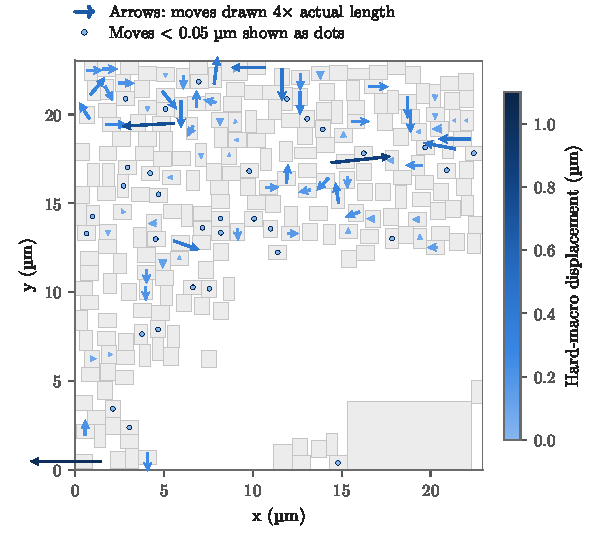
\includegraphics{figures/ibm01_displacement.pdf}}%
\begin{minipage}[c]{\wd\sidefigbox}\usebox{\sidefigbox}\end{minipage}\hfill
\begin{minipage}[c]{\dimexpr\linewidth-\wd\sidefigbox-1.2em\relax}
\captionsetup{justification=raggedright,singlelinecheck=false}
\caption{Hard-macro displacement on IBM01 between the saved endpoints of the first
curvature stage (proxy 0.85527) and the cascade (proxy 0.84528), \historical. Arrows
start at the first-stage position and are drawn four times longer than the actual
displacement, moves under $0.05\,\mu$m are drawn as dots, and color gives the
length. The difference includes the CD polish after
every accepted step, so it is not a trajectory.}
\label{fig:ibm01-displacement}
\end{minipage}
\end{figure}

Figure~\ref{fig:ibm01-displacement} shows what the cascade changed on IBM01, a design
whose two endpoints are both strictly valid. It moved 104 of the 246 hard macros, by at
most $1.01\,\mu$m on a canvas $23\,\mu$m wide; the median displacement among the moved
macros is $0.085\,\mu$m. It also moved 407 of the 894 soft clusters, by up to
$8.4\,\mu$m (not drawn). The score fell by 0.00999 through many small, scattered
adjustments rather than a rearrangement of blocks.

\section{Post-competition verification}\label{app:verification}

In September 2026 we audited the competition code against the challenge rules and
our own runtime assumptions, repaired what we found in a separate post-competition
runtime, and exercised the repairs in short engineering runs on an Apple M3 Max.
This appendix lists the defects with their bearing on the judged entry, gives the
evaluator microbenchmarks behind the main text's speed and agreement figures, and
condenses the engineering runs, including a first reproduction attempt that was
stopped.

\subsection{Defects and their scope}\label{app:defects}

\begin{table}[htbp]
\centering\footnotesize
\setlength{\tabcolsep}{3pt}
\caption{Defects found by the post-competition audit. ``Judged entry'' answers whether
the defect could have affected the 20 May IBM entry: \emph{no}, \emph{unknown}, or
\emph{note} for an item that is not a defect. Tests are those of
Appendix~\ref{app:repro}; ``IBM input record'' is
\texttt{ibm\_repair\_equivalence.json}.}
\label{tab:defects}
\begin{tabularx}{\linewidth}{@{}>{\raggedright\arraybackslash}p{0.16\linewidth}
                >{\raggedright\arraybackslash}p{0.17\linewidth}
                Y
                >{\raggedright\arraybackslash}p{0.17\linewidth}
                >{\raggedright\arraybackslash}p{0.20\linewidth}@{}}
\toprule
Defect & Where & Judged entry & Fix & Evidence \\
\midrule
Lane join became \path{timeout=None} after the deadline & Three-lane supervisor &
No: the single pipeline has no lanes to join & Shared monotonic deadline; zero join
timeout after expiry; external process-group timeout & Join and termination tests;
IBM17 runs stopped at 240.0--240.1\,s (limit 240\,s) \\
\addlinespace
Stage polish caps exceed the stage budget & Curvature stage; v1 cascade and portfolio
& No: neither stage is in the single pipeline & Caps charged for eigensolver and
legalizer time; deadline checked between HVPs & Three budget tests \\
\addlinespace
Lane result written only on normal completion & Lane worker & No: the single
pipeline returns its placement directly & Atomic, validated checkpoint per phase; best
valid one recovered & Checkpoint tests; three recoveries in each 12-run batch \\
\addlinespace
Temporary lane directories not removed & Three-lane supervisor & No: no lane
directories, and disk residue cannot change a placement & Cleanup on every exit path &
Cleanup tests \\
\addlinespace
Pin owner taken from the pin name before its first ``/'' & Surrogate net extraction
(\path{_extract_net_data}) & No: IBM names are flat, verified on 17 of 17 designs
(0 owner mismatches over 411,642 macro pins; identical net tensors); IBM01 keeps
2,978 hard-pin occurrences and 5,993 retained nets & Owner from the parser's pin
object & IBM input record; ariane133: all 5,498 used hard-pin occurrences restored;
four tests \\
\addlinespace
Same split in the initializer's macro graph & \path{sdf_init.py} & No: IBM names are
flat; edge lists identical on 17 of 17 designs (IBM01: 644 edges) & Map from the
parser's hard-macro pins & IBM input record; ariane133: 0 to 859 edges; replayable
record; four tests \\
\addlinespace
\texttt{qualified} set from the overlap count alone & Local result writer & No: the
organizers scored with their own harness & Validity and eligibility recorded
separately & 22 of 34 overlap-free historical endpoints pass strict containment \\
\addlinespace
Input soft clusters outside the canvas not repaired & Initializer; push-apart &
Unknown: no judged coordinates survive; 15 of 17 IBM inputs have 1 to 11 such
clusters, which the descent pushes inward without guaranteeing containment; the
organizers verified the entry & Every movable center projected into the canvas &
IBM input record; v1 failed on IBM10 and IBM17 in the pilot and passed on IBM10 after
repair; soft-bound tests \\
\addlinespace
Float32 export can round past the upper canvas edge & Final conversion after clipping &
Unknown: the single pipeline also exports float32; the organizers verified the entry &
Step one representable value inward & 12 of 34 historical endpoints exceed by one step;
one test \\
\addlinespace
NG45 lookup failed on the \path{_ng45} name suffix & \path{find_benchmark_dir} & No:
IBM names have no suffix & Explicit aliases, exact name first & Pilot ariane133
failures; later batches valid; three tests \\
\addlinespace
Golden-section search unreachable & CD axis search & Note: it never runs & None
needed & At most ten candidates; list capped at 12 \\
\bottomrule
\end{tabularx}
\end{table}

Table~\ref{tab:defects} lists each defect, where it lived in the competition code,
whether it could have affected the judged 20 May IBM entry, the repair and the
evidence that the repair works. The judged entry is inferred to be the single
pipeline of Appendix~\ref{app:alg-supervisor}; its listed runtime of about 12 minutes
per design matches its 720\,s budget. Two facts settle most rows: that pipeline runs
in one process without lane workers, and every hard-macro name in the 17 IBM netlists
is flat, so the first ``/'' of a pin name always separates the owning macro. A
frozen record checks this on all 17 pinned IBM inputs
(\path{writeup/data/publication/ibm_repair_equivalence.json}, written by
\path{scripts/measure_publication_ibm_repair_equivalence.py}; \measurement). It
compares the extraction code of 20 May (commit \texttt{5485310}) with the corrected
runtime without optimizing or scoring: the two ownership rules agree on all 411,642
macro pins, and the smooth net tensors and the initializer's hard-macro edge lists
are identical on 17 of 17 designs. The same record finds no fixed macros, and soft
clusters outside the canvas in the inputs of 15 designs (1 to 11 per design), which
the corrected runtime's initial clamp moves. The ``Evidence'' column refers to the
focused tests of Appendix~\ref{app:repro} and to the frozen diagnostics.


\subsection{Matched incremental-evaluator measurements}
\label{sec:evaluator}
We measured identical prescribed move sequences through two evaluation paths: incremental updates returning wirelength, density, congestion, and proxy; and the canonical placement setter followed by the three full component computations. Neither timed path includes hard-overlap validation. Both use float64 positions on the Mac CPU with one PyTorch thread. The order of the two engines alternates between repetitions; initialization and a warm-up component evaluation precede each batch.

\begin{table}[htbp]\centering\footnotesize
\caption{CPU component-kernel microbenchmarks. Times are means per move. Each ratio is the full-recomputation time divided by the incremental time for one paired batch; the table gives the median and range over three paired batches for the IBM01 sample and two paired batches for each IBM10 sample (the median of two batches is their mean). Setup and overlap checks are excluded; these are kernel measurements, not end-to-end placer speedups.}
\label{tab:incremental-measurements}
\begin{tabular}{llrrrr}
\toprule
Design / sample & Moves $\times$ repeats & Inc. time (ms) & Full time (ms) & Median ratio & Range \\
\midrule
IBM01 / mixed & $8 \times 3$ & 1.29 & 1{,}401.6 & 1{,}040$\times$ & 1{,}035--1{,}197 \\
IBM10 / soft & $3 \times 2$ & 3.67 & 26{,}682.1 & 7{,}269$\times$ & 7{,}055--7{,}483 \\
IBM10 / hard & $3 \times 2$ & 1.49 & 26{,}865.4 & 18{,}023$\times$ & 17{,}250--18{,}795 \\
\bottomrule\end{tabular}\end{table}

Every measured component agreed within relative tolerance $10^{-5}$, using $|a-b|/\max(|a|,|b|,10^{-30})$; the largest observed relative discrepancy was $2.6\times 10^{-15}$. Evaluator setup is excluded from the ratios and retained in the raw records. The sequences are small: IBM01 has three hard-macro moves and five soft-cluster moves per repetition; the first IBM10 sequence happened to select only soft clusters, so a separate hard-only sequence was measured. Moves may create overlaps. The ratios compare localized cache updates with full recomputation in the reference Python evaluator, so they reflect both the update strategy and the implementation, and they exclude the rest of the placer.

Mean incremental setup times were IBM01 mixed: 0.33 s, IBM10 soft: 1.48 s, IBM10 hard: 1.45 s. A separate overlap-metrics call on each final state is also timed in the raw data; it is excluded from both component paths and is not the full geometry-validation cost. Repetitions share the same seed and moves, so their spread measures timing repeatability, not independent placement outcomes.


\subsection{Engineering runs}\label{app:engineering}

Three batches exercised the repaired runtime with the corrected runner. They are short
engineering checks: the solver budgets are 60 to 180\,s, far below the competition's
hour, and their purpose is execution, recording and legality, not quality. All ran on
an Apple M3 Max (14 logical CPUs, 36\,GiB) under macOS 26.6.2 with CPython 3.9.6 and
PyTorch 2.8.0, nominal seed 42, and every planned run is reported. Each batch froze its
source as a runtime archive before execution: \texttt{5730d13762ce} for the pilot,
\texttt{ca4343aaefda} for the repair batch and \texttt{5aa4c719cf18} for the NG45
integration check.

\paragraph{Pilot.} The predeclared designs were IBM01 (small), IBM10 (large), IBM17
(historically hardest) and ariane133, a hierarchical NG45 design. Each configuration
used 500 analytical steps and a 30\,s CD phase cap, and runs went one at a time.
Table~\ref{tab:pilot-results} gives the outcomes. The seven errors have three causes.
The v1 runs on IBM10 and IBM17 failed canvas containment after local refinement,
because their inputs contain movable soft clusters outside the canvas that the
original initializer does not repair. On IBM17 both v2 configurations exhausted their
budget without a valid checkpoint. All three ariane133 runs failed to locate the
design directory, before any optimization. No run reached the external limit. Two
recoveries show how the checkpoints behave: on IBM01 the three-lane run returned
Lane~B's checkpoint after its curvature step (0.827866) when the lanes were stopped at
the solver budget, and on IBM10 the standalone and three-lane runs returned the same
legalized-descent state (1.166864). Final validation and export took 26.5--28.2\,s on
IBM10 against about 1.5\,s on IBM01.

% Generated by scripts/render_publication_pilot.py; do not edit.
% Limited-budget engineering evidence; no official-budget extrapolation.
\begin{table}[htbp]
\centering
\footnotesize
\caption{Limited-budget pilot on four designs (180\,s solver budget, 240\,s external limit, 1 concurrent job, 3 CPU threads per run). C: completed pipeline; P: valid result after partial phases; R: valid checkpoint recovery; E: error. Returned: lane and phase whose saved coordinates equal the returned placement. Threads: CPU threads per solver process as recorded. Every planned run is shown.}
\label{tab:pilot-results}
\begin{tabular}{@{}llrrrclr@{}}
\toprule
Design & Variant & Proxy & Solver (s) & Wall (s) & Outcome & Returned & Threads \\
\midrule
IBM01 & v1 & 0.92786 & 140.8 & 145.1 & P & E25 & 3 \\
IBM01 & A & 0.83617 & 51.3 & 54.4 & C & A/final & 3 \\
IBM01 & A+B+C & 0.82787 & 180.0 & 183.0 & R & B/curvature & 1 \\
IBM10 & v1 & --- & --- & 70.1 & E & --- & 3 \\
IBM10 & A & 1.16686 & 180.0 & 209.5 & R & A/descent & 3 \\
IBM10 & A+B+C & 1.16686 & 180.0 & 211.0 & R & ABC/descent & 1 \\
IBM17 & v1 & --- & --- & 71.0 & E & --- & 3 \\
IBM17 & A & --- & --- & 183.8 & E & --- & --- \\
IBM17 & A+B+C & --- & --- & 183.6 & E & --- & --- \\
ariane133 & v1 & --- & --- & 2.1 & E & --- & 3 \\
ariane133 & A & --- & --- & 3.1 & E & --- & --- \\
ariane133 & A+B+C & --- & --- & 3.0 & E & --- & --- \\
\bottomrule
\end{tabular}
\end{table}

Coverage by variant: v1 1/4 eligible, 0/4 completed; A 2/4 eligible, 1/4 completed; A+B+C 2/4 eligible, 0/4 completed. No variant has an eligible result on every planned design, so no mean is reported. Where initializer or legalized-descent checkpoints survive for all three A+B+C lanes and for standalone A (IBM01 initializer, IBM01 legalized descent, IBM10 legalized descent), the four coordinate tensors are bit-identical; the nominal lane seeds therefore did not diversify the shared prefix. Full SHA-256 values are in the JSON summary.


\paragraph{Repair batch.} The second batch adds the all-movable bounds repair,
fixed-reference preservation, the NG45 aliases and retained phase diagnostics, and runs
the same 12 cells three at a time, still with three CPU threads per run
(Table~\ref{tab:repair-validation-results}). Standalone A used all three threads in
its one lane; the three-lane runs gave one thread to each lane. That allocation, and
the phase each run reached, explain the IBM10 contrast: A returned its legalized
descent (1.14944) while the three-lane run returned its initializer (1.41116), so the
two values measure progress under different resources, not the value of the extra
lanes. The ariane133 rows still use the original soft-rectangle edge extractor; its
repair came after this batch.

% Generated by scripts/render_publication_pilot.py; do not edit.
% Limited-budget engineering evidence; no official-budget extrapolation.
\begin{table}[htbp]
\centering
\footnotesize
\caption{Post-pilot repair validation results. C: completed pipeline; P: valid partial-phase result; R: valid checkpoint recovery; T: timeout. Every planned run is shown.}
\label{tab:repair-validation-results}
\begin{tabular}{llrrrc}
\toprule
Design & Variant & Proxy & Solver time (s) & Wall time (s) & Outcome \\
\midrule
ibm01 & v1 & 0.93106 & 151.8 & 155.2 & P \\
ibm01 & A & 0.83681 & 53.6 & 56.9 & C \\
ibm01 & A+B+C & 0.82961 & 180.0 & 183.2 & R \\
ibm10 & v1 & 1.22215 & 125.3 & 169.1 & P \\
ibm10 & A & 1.14944 & 180.0 & 225.6 & R \\
ibm10 & A+B+C & 1.41116 & 180.0 & 216.2 & R \\
ibm17 & v1 & -- & -- & 240.1 & T \\
ibm17 & A & -- & -- & 240.0 & T \\
ibm17 & A+B+C & -- & -- & 240.0 & T \\
ariane133\_ng45 & v1 & 0.65572 & 172.8 & 181.6 & P \\
ariane133\_ng45 & A & 0.64930 & 81.1 & 89.0 & C \\
ariane133\_ng45 & A+B+C & 0.64911 & 180.0 & 187.8 & P \\
\bottomrule
\end{tabular}
\end{table}

\begin{table}[htbp]
\centering
\small
\caption{Post-pilot repair validation coverage. A mean requires an eligible finite proxy for every planned design; outcome codes follow Table~\ref{tab:repair-validation-results}.}
\label{tab:repair-validation-coverage}
\begin{tabular}{lrrrrr}
\toprule
Variant & Recorded & Eligible & Pipeline & Error/TO & Mean proxy \\
\midrule
v1 & 4/4 & 3/4 & 0/4 & 1 & -- \\
A & 4/4 & 3/4 & 2/4 & 1 & -- \\
A+B+C & 4/4 & 3/4 & 0/4 & 1 & -- \\
\bottomrule
\end{tabular}
\end{table}

\begin{table}[htbp]
\centering
\small
\caption{Recorded coordinate-hash prefixes for A+B+C. I and D denote initializer and legalized-descent checkpoints; full SHA-256 values remain in the JSON artifact. Distinct requires all three lanes, and a double dash denotes unavailable metadata.}
\label{tab:repair-validation-prefix-diversity}
\begin{tabular}{llcccrl}
\toprule
Design & Phase & A hash & B hash & C hash & Distinct & vs standalone A \\
\midrule
ibm01 & I & \texttt{d8fc4aa3} & \texttt{d8fc4aa3} & \texttt{d8fc4aa3} & 1 & all= \\
ibm01 & D & \texttt{857303c2} & \texttt{857303c2} & \texttt{857303c2} & 1 & all= \\
ibm10 & I & \texttt{267c4230} & \texttt{267c4230} & \texttt{267c4230} & 1 & all= \\
ibm10 & D & -- & -- & -- & -- & -- \\
ibm17 & I & -- & -- & -- & -- & -- \\
ibm17 & D & -- & -- & -- & -- & -- \\
ariane133 & I & \texttt{a9b2a1ab} & \texttt{a9b2a1ab} & \texttt{a9b2a1ab} & 1 & all= \\
ariane133 & D & \texttt{ca3f2d67} & \texttt{ca3f2d67} & \texttt{ca3f2d67} & 1 & all= \\
\bottomrule
\end{tabular}
\end{table}

Equality in Table~\ref{tab:repair-validation-prefix-diversity} refers only to finalized checkpoint inventories; missing metadata does not show that no checkpoint was saved. Nominal lane seeds do not establish independent basin starts; effective initializer seeds are retained in JSON. The equality motivates future shared-prefix evaluation, but this validation measures no speedup.


\paragraph{NG45 integration.}
\subsection{Final NG45 integration}
A separate check of runtime archive \code{5aa4c719cf18} ran all three entry configurations on ariane133 with a 60-second solver budget, a 120-second external limit, and three concurrent jobs. A and A+B+C used five analytical steps and zero-second CD phase budgets; v1 retained its distinct budget-derived refinement stages. All three outputs were valid and study-eligible. Only A completed its configured pipeline; v1 and A+B+C returned valid partial-phase outputs. These are integration checks, not comparable quality measurements.

\begin{table}[htbp]\centering\small
\caption{Final NG45 integration after the SDF graph repair; every row returned a valid placement within its external limit.}
\label{tab:final-ng45-integration}
\begin{tabular}{lrrl}\toprule
Variant & Solver time (s) & Wall time (s) & Outcome \\ \midrule
v1 & 34.6 & 44.0 & partial phases \\
A & 45.7 & 53.7 & complete \\
A+B+C & 60.0 & 67.8 & partial phases \\
\bottomrule\end{tabular}\end{table}


\paragraph{IBM17 timeouts and finalization cost.} The three IBM17 runs of the repair
batch are the only runs that reached the external limit, and the saved artifacts show
where the time went. Both v2 configurations logged lane selection before the limit, so
the remaining time was spent after the placer returned, where the worker validates the
placement and calls the canonical scorer once more before saving it. The v1 run wrote
its first checkpoint at 192.7\,s, although its inner log reports 66.4\,s of search; the
gap covers differing timer origins and the canonical scoring that precedes every
checkpoint write. One canonical score of IBM17 takes
about 73\,s on this host with one thread (72.8 and 73.3\,s for the two IBM17 endpoints
rescored in Appendix~\ref{app:curvature}), against 1.3\,s for IBM01. That single call
is longer than the 60\,s between the 180\,s solver budget and the 240\,s limit. For the
planned one-hour runs, the study configuration therefore stops the solver at 3,300\,s
and reserves the last five minutes for validation and export.

\paragraph{First reproduction attempt (engineering record).}\label{app:repro-attempt}
A reproduction of the ranked configuration (single pipeline, 720\,s per design, all
17 IBM designs, one design at a time on the CPU with three threads) was started on
30 September 2026 on the same M3 Max, by then under macOS 27.0.1, and stopped by the
operator during IBM06, which has no result. IBM03 had exposed a defect in the
corrected runtime: its per-phase checkpoint validates canvas bounds strictly, without
the one-step inward projection applied at export, so any bounds excess at that
point, such as a float32 rounding overshoot at the upper canvas edge, discards the
coordinate-descent result. On IBM03 coordinate descent completed, its final
checkpoint failed strict validation, and the run returned its checkpoint from before
coordinate descent (proxy 1.10002); the rejected candidate was not saved, so its
excess is unknown. IBM01, IBM02 and IBM04 completed the pipeline (0.82996, 1.00200 and
0.91909). These four designs are not a suite result, are not a \reproduction{}
result and are not compared with any other record; a fix is pending. The records are
under \path{writeup/runs/ranked-reproduction-20260930/}.

\section{Suite records and evidence ledger}\label{app:records}

% Evidence-label macros; the main preamble normally defines them.
\providecommand{\official}{\textsc{Official}}
\providecommand{\historical}{\textsc{Historical}}
\providecommand{\measurement}{\textsc{Measurement}}
\providecommand{\reproduction}{\textsc{Reproduction}}

\subsection{Historical suite records}\label{app:records-historical}

Three complete 17-design records survive from May 2026
(Table~\ref{tab:historical-baselines}). Each is an evaluator output with per-design
components, overlap counts, runtimes, a timestamp, four concurrent jobs and one Torch
thread; none stores coordinates, a source revision or host details, so the scores can
be recomputed from their components but not from placements. Contemporaneous notes
place the 17 May v1 run on the M3 Max and the early v2 run on an AWS EPYC instance;
the 0.98199 record names no host. The records differ in program, hardware and
time budget, so differences between columns describe the records, not the effect of
any one change.

\begin{table}[htbp]
\centering
\footnotesize
\caption{Historical records; hardware, budgets and concurrency differ. Proxy cost per design (lower is better) for three development records and the two published baselines listed by the challenge. Each record is below both baselines on all 17 designs.}
\label{tab:historical-baselines}
\begin{tabular}{lrrrrr}
\toprule
Design & SA & RePlAce & v1 (17 May) & Early v2 & \shortstack{Single pipeline\\(20 May lineage)} \\
\midrule
IBM01 & 1.3166 & 0.9976 & 0.85963 & 0.84658 & 0.82152 \\
IBM02 & 1.9072 & 1.8370 & 1.00659 & 0.99484 & 1.01265 \\
IBM03 & 1.7401 & 1.3222 & 0.92742 & 0.90815 & 0.88836 \\
IBM04 & 1.5037 & 1.3024 & 0.97285 & 0.94491 & 0.92131 \\
IBM06 & 2.5057 & 1.6187 & 1.13361 & 1.07574 & 1.05296 \\
IBM07 & 2.0229 & 1.4633 & 1.05294 & 1.03333 & 1.01486 \\
IBM08 & 1.9239 & 1.4285 & 1.08163 & 1.04295 & 1.02490 \\
IBM09 & 1.3875 & 1.1194 & 0.82494 & 0.78161 & 0.77033 \\
IBM10 & 2.1108 & 1.5009 & 0.99575 & 0.98969 & 0.97934 \\
IBM11 & 1.7111 & 1.1774 & 0.86041 & 0.80567 & 0.78831 \\
IBM12 & 2.8261 & 1.7261 & 1.19196 & 1.14974 & 1.08989 \\
IBM13 & 1.9141 & 1.3355 & 0.93633 & 0.85447 & 0.84279 \\
IBM14 & 2.2750 & 1.5436 & 1.19081 & 1.10989 & 1.07330 \\
IBM15 & 2.3000 & 1.5159 & 1.15820 & 1.08974 & 1.05557 \\
IBM16 & 2.2337 & 1.4780 & 1.12240 & 1.03277 & 0.99607 \\
IBM17 & 3.6726 & 1.6446 & 1.32264 & 1.24247 & 1.17164 \\
IBM18 & 2.7755 & 1.7722 & 1.33932 & 1.23934 & 1.18998 \\
\midrule
Mean & 2.1251 & 1.4578 & 1.05750 & 1.00835 & 0.98199 \\
\bottomrule
\end{tabular}
\end{table}


Against the published baselines, the margin below RePlAce ranges from 13.8\% (v1,
IBM01) to 45.8\% (early v2, IBM02). The 0.98199 record is lower than the v1
record on 16 of 17 designs. The exception is IBM02: density falls from 0.61156 to
0.57491, but wirelength rises from 0.08418 to 0.08897 and congestion from 1.23324 to
1.27245, so the total rises from 1.00659 to 1.01265. The largest change is on IBM17,
where congestion falls from 1.88679 to 1.66501 and density from 0.60911 to 0.53604, a
total decrease of 0.15100; IBM17 nevertheless remains among the costliest designs.

\paragraph{Repeatability.} One direct repeatability observation survives, as a
\historical{} note rather than a frozen record: a development note (commit
\texttt{4a202de}) records an identical rerun of the 17 May v1 configuration on the same
M3 Max over a four-design subset. The subset mean moved from 0.89844 to 0.89517
($-0.36\%$); IBM01 moved from 0.85963 to 0.84691 ($-1.48\%$), IBM04 was unchanged, and
IBM09 and IBM13 moved by $-0.20\%$ and $+0.14\%$. This is one repeat pair of a
different pipeline from the ranked one. It shows that run-to-run differences of a few
tenths of a percent in a subset mean, and over 1\% on one design, occur without any
code change; it is not a confidence interval.

\paragraph{Lineage of the judged entry.} The final leaderboard row reads
``Resubmitted 5/20 (thinkorplace-v2). Was 1.0771'' and names no commit, archive or
result digest. We infer that the judged program was the 20 May single pipeline, most
likely commit \texttt{5485310}, from three premises: the resubmission
date; the listed runtime of about 12 minutes per design, which matches that pipeline's
720\,s budget rather than the three-lane system's 2,700\,s; and the upstream leaderboard
of 21 May, which listed the pending resubmission with a self-reported score consistent
with the single-pipeline lineage and not with the early-v2 record at 1.00835 (the
provenance note in Appendix~\ref{app:records-ledger} gives the figure). The exact
judged commit was not recorded, and the three-lane commits of 22 May (Eastern time)
still preceded the Pacific-time deadline, so chronology alone cannot exclude them; the
inference rests on the listed 12-minute runtime and the 20 May resubmission date.

\subsection{Reproduction}\label{app:records-reproduction}

Table~\ref{tab:reproduction} gives each design of the rerun in
\cref{sec:reproduction} (\reproduction), rendered from its run records by
\path{scripts/render_publication_reproduction.py}.

\begin{table}[htbp]
\centering
\footnotesize
\caption{Reproduction (post-competition), ranked configuration rerun on the lead author's Apple M3 Max CPU, one design at a time; all values from the canonical evaluator. Proxy = wirelength + $\tfrac{1}{2}$\,density + $\tfrac{1}{2}$\,congestion. Ratio to RePlAce: each proxy over the published RePlAce value for its design; in the mean row, the mean proxy over the RePlAce mean (1.4578). Wall: supervised time per design, including final validation (720\,s solver budget, 3,600\,s limit). $\checkmark$: full pipeline completed.}
\label{tab:reproduction}
\begin{tabular}{lrrrrrrc}
\toprule
Design & Proxy & Wirelength & $\tfrac{1}{2}$\,Density & $\tfrac{1}{2}$\,Congestion & Ratio to RePlAce & Wall (s) & Outcome \\
\midrule
IBM01 & 0.82996 & 0.08442 & 0.26335 & 0.48218 & 0.832 & 329 & $\checkmark$ \\
IBM02 & 1.00200 & 0.08971 & 0.28751 & 0.62479 & 0.545 & 364 & $\checkmark$ \\
IBM03 & 0.91446 & 0.10122 & 0.25211 & 0.56113 & 0.692 & 352 & $\checkmark$ \\
IBM04 & 0.91909 & 0.08946 & 0.25343 & 0.57620 & 0.706 & 346 & $\checkmark$ \\
IBM06 & 1.03906 & 0.08057 & 0.25438 & 0.70411 & 0.642 & 348 & $\checkmark$ \\
IBM07 & 1.00657 & 0.08705 & 0.26236 & 0.65716 & 0.688 & 361 & $\checkmark$ \\
IBM08 & 1.01842 & 0.08599 & 0.25798 & 0.67445 & 0.713 & 375 & $\checkmark$ \\
IBM09 & 0.77703 & 0.06776 & 0.25831 & 0.45097 & 0.694 & 365 & $\checkmark$ \\
IBM10 & 0.98044 & 0.08049 & 0.25927 & 0.64068 & 0.653 & 743 & $\checkmark$ \\
IBM11 & 0.78998 & 0.06582 & 0.25516 & 0.46900 & 0.671 & 396 & $\checkmark$ \\
IBM12 & 1.08597 & 0.07966 & 0.26455 & 0.74177 & 0.629 & 721 & $\checkmark$ \\
IBM13 & 0.84098 & 0.06592 & 0.26020 & 0.51486 & 0.630 & 404 & $\checkmark$ \\
IBM14 & 1.06636 & 0.06678 & 0.26922 & 0.73037 & 0.691 & 726 & $\checkmark$ \\
IBM15 & 1.05107 & 0.07465 & 0.29701 & 0.67941 & 0.693 & 573 & $\checkmark$ \\
IBM16 & 1.00323 & 0.06560 & 0.27215 & 0.66549 & 0.679 & 754 & $\checkmark$ \\
IBM17 & 1.17400 & 0.07126 & 0.26957 & 0.83316 & 0.714 & 782 & $\checkmark$ \\
IBM18 & 1.18197 & 0.07536 & 0.29480 & 0.81180 & 0.667 & 539 & $\checkmark$ \\
\midrule
Mean & 0.98121 & 0.07834 & 0.26655 & 0.63633 & 0.673 & 499 &  \\
\bottomrule
\end{tabular}
\end{table}


\subsection{Evidence ledger}\label{app:records-ledger}

Table~\ref{tab:evidence-ledger} maps each quantitative claim of the report to its
evidence label and record.

\begin{table}[htbp]
\centering\footnotesize
\caption{Claim-to-evidence map. \official: the organizers' final leaderboard.
\historical: May 2026 development records. \measurement: post-competition diagnostics
on frozen inputs. \reproduction: the post-competition run of the ranked
configuration.}
\label{tab:evidence-ledger}
\begin{tabular}{@{}>{\raggedright\arraybackslash}p{0.30\linewidth}
                >{\raggedright\arraybackslash}p{0.13\linewidth}
                >{\raggedright\arraybackslash}p{0.22\linewidth}
                >{\raggedright\arraybackslash}p{0.27\linewidth}@{}}
\toprule
Claim & Label & Record & Scope \\
\midrule
Ninth on the final leaderboard, verified mean 0.9974; best 0.7829, worst 1.2602 &
\official & Upstream README at \texttt{996193c} & Inferred to be the 20 May single
pipeline; judged commit not recorded \\
Winner 0.9507; SA and RePlAce baseline means 2.1251 and 1.4578 & \official &
Same README; baselines from \citet{cheng2025updated} & Organizers' numbers, not
reruns \\
v1 (17 May) mean 1.05750 & \historical & Frozen evaluator JSON & Components only; no
coordinates \\
Early v2 mean 1.00835 & \historical & Frozen evaluator JSON & Earlier smooth placer
(V3); different host \\
0.98199 record, lower than v1 on 16 of 17 & \historical &
Frozen evaluator JSON & Closest surviving full-suite record of the ranked lineage;
unmatched conditions \\
Congestion supplies 84.5\% of the decrease from the v1 record to the 0.98199 record & \historical &
Component fields of the two records & Arithmetic attribution, not a mechanism \\
Plateau 1.08128, first curvature stage 1.06760, cascade 1.06119 & \historical &
Frozen stage records and 34 placements & Uncapped research runs \\
Rescoring within $9.87\times10^{-8}$; 22 of 34 endpoints strictly valid &
\measurement & Rescore and geometry records & Coordinates left unrepaired \\
190 of 204 first-stage attempts below the plateau & \historical & Frozen stage
records & No random-direction or zero-step control; 12 attempts per design \\
Incremental update 1.29--3.67\,ms versus 1.40--26.87\,s; largest error
$4.44\times10^{-16}$ & \measurement & Frozen microbenchmarks & 14 sampled moves on
IBM01 and IBM10, single-move path only; not a uniform bound \\
IBM01 curvature: active-branch eigenvalue $-0.442458$; wirelength HVPs agree to
$4\times10^{-9}$ & \measurement & Frozen diagnostic and follow-up & One surrogate, one
endpoint \\
Ten defects and repairs (5,498 pin occurrences, 859 edges) & \measurement &
Topology records; focused tests & Extraction and execution, not placement quality \\
Repairs leave all 17 IBM inputs unchanged; 15 have soft clusters outside the canvas
& \measurement & IBM repair-equivalence record & Input extraction only; no
optimization or scoring \\
Engineering batches & \measurement & Frozen run records & 60--180\,s budgets; no suite
mean \\
Repeatability $-0.36\%$ (subset), $-1.48\%$ (IBM01) & \historical & Development note,
not frozen & One repeat pair of v1 \\
Rerun of the ranked configuration on a laptop CPU: mean \ReproMean{} &
\reproduction & Its own run records & Reported in Section~\ref{sec:reproduction} and
Table~\ref{tab:reproduction} \\
Full-suite score of the three-lane system & --- & None & Never scored (inferred) \\
\bottomrule
\end{tabular}
\end{table}

Provenance only: three further numbers appear in May-era notes and listings. The
upstream leaderboard of 21 May showed the pending resubmission with a self-reported
0.991; 0.98387 is an extended-CD standalone run; and 0.97745 is an offline per-design
minimum across component runs. None has a frozen record or is a result of this
report.

\begingroup
\raggedright
\setlength{\parindent}{1.1em}
\section{Reproducibility}\label{app:repro}

The code, frozen evidence and report sources are in the public repository
\url{https://github.com/brmurrell3/macro-placer}. Commands below run from the
repository root with the project's virtual environment.

\paragraph{Source revisions.} Three revisions anchor the work. The competition
snapshot \texttt{2ab92a33d352} (22 May 2026) is the last competition-era commit; its
Python source closure is frozen as \path{writeup/data/publication/competition-source.tar},
described by \path{source_snapshot.json} with the archive digest and file list. The
upstream challenge revision \texttt{996193c83eaa} (14 August 2026) carries the final
leaderboard. The TILOS MacroPlacement submodule is pinned at \texttt{45a721d01dfe};
six canonical evaluator, loader and validation files are byte-identical between the
local base and the final challenge revision. The ranked single pipeline is most
likely commit \texttt{5485310}; Appendix~\ref{app:records} gives the basis for that
inference.

\paragraph{Package extraction.} The competition entries imported code from the
experiment tree, so copying a submission directory onto a clean checkout of the
challenge was not enough to run it. The post-competition cleanup extracts the active
dependency closure into the package \path{thinkorplace/} with three parts,
\path{thinkorplace.common}, \path{thinkorplace.v1} and \path{thinkorplace.v2}, using
relative imports; the submission entry points remain as thin adapters. Runtime
imports no longer touch \path{experiments/} or \path{writeup/}.
\path{thinkorplace/MIGRATION.json} records the origin and source digest of every
module. The package keeps the optimization formulas and adds the repairs of
Appendix~\ref{app:verification}; a test checks that the extracted primitives
preserve the original algorithms' syntax trees.

\paragraph{Frozen evidence and generators.} \path{writeup/data/publication/} holds
the evidence, and its \path{README.md} states the scope of each record:
\begin{itemize}
  \item \path{raw/}: the three historical suite records, the 34 curvature-stage
        records and the 34 saved placement tensors, with SHA-256 values in
        \path{historical_summary.json};
  \item the evaluator microbenchmarks, curvature diagnostic and follow-up,
        rescoring and geometry records, topology diagnostics, tail-bound and
        error-margin arithmetic, and the frozen leaderboard;
  \item \path{ibm_repair_equivalence.json}, written by
        \path{scripts/measure_publication_ibm_repair_equivalence.py}: on all 17 IBM
        inputs, the 20 May extraction code (commit \texttt{5485310}) and the
        corrected runtime agree on pin ownership, smooth net tensors and initializer
        edges, and the record counts the input soft clusters that the initial clamp
        moves; no optimization or scoring is run;
  \item summaries of the three engineering batches, whose primary run records
        (manifests, requests, results, logs, placements and checkpoint hashes) are
        under \path{writeup/runs/}, as are those of the stopped first reproduction
        attempt (\path{writeup/runs/ranked-reproduction-20260930/});
  \item \path{corrected-runtime-*.tar.gz}: deterministic archives of each
        post-competition runtime, with per-file digests in the matching
        \path{corrected_runtime_snapshot_*.json}.
\end{itemize}
Generators read these records and write only derived summaries, tables and figures;
the historical freezer refuses to replace a frozen raw record with different bytes.
No generator runs a solver, and the scripts that produced the diagnostics are separate
from the generators.

\paragraph{Runner.} The study runner (\path{scripts/run_publication_study.py} with
\path{scripts/publication_worker.py}) implements the following workflow:
\begin{enumerate}
  \item create an immutable run manifest before any solver is constructed;
  \item record input and initialization hashes and the explicit device choice;
  \item save canonical incumbents atomically at every meaningful phase;
  \item propagate one monotonic solver deadline and enforce an external
        process-group timeout;
  \item validate the final candidate independently and retain every failure;
  \item preserve final coordinates and phase metadata for deterministic
        post-processing.
\end{enumerate}
A run's identity covers executable source, dependencies, inputs and constructor
settings, so editing the paper does not invalidate a run while any runtime change
does. Source is hashed again after execution. Validity (shape, finite values,
containment, fixed objects, zero hard overlaps), study eligibility (return within the
external limit with matching source and environment) and pipeline completion are
separate fields: a valid recovered checkpoint can be an eligible anytime result
without a completed pipeline.

\paragraph{Tests.} Runtime archive \texttt{5aa4c719cf18} passed 64 focused tests in
five modules; the receipt \path{verification/final-tests-20260906.json} binds the
archive to the test log:
\begin{itemize}
  \item \path{test_submission_safety.py} (30): deadline propagation, zero join
        timeouts after expiry, child termination and cleanup, rejection of invalid
        lanes, checkpoint retention and atomic replacement, phase-outcome
        reporting, hierarchical pin ownership in four code copies, and budget guards
        for the curvature stages and the eigensolver;
  \item \path{test_thinkorplace_package.py} (7): imports against a pristine
        upstream without the research tree, legalizer clamping of soft clusters,
        parity of runtime validation with the canonical check on float32 endpoints
        and randomized geometry, and preservation of the extracted algorithms;
  \item \path{test_postpilot_repairs.py} (12): soft-cluster bounds, fixed obstacles,
        float32 export, infeasible fixed references, unresolved hard geometry, NG45
        directory aliases, and retained diagnostics for rejected initializers and
        fatal results;
  \item \path{test_sdf_topology.py} (4): initializer edge extraction for flat and
        hierarchical netlists in both code copies;
  \item \path{test_publication_runner.py} (11): explicit parameters, worker
        validation, checkpoint-recovery semantics, process-group timeouts, resume
        identity, dry runs and checkpoint inventories.
\end{itemize}
These are engineering checks of execution and validation, not measurements of
placement quality.

\paragraph{Commands.} Regenerate the tables and figures from the frozen records:
\begin{verbatim}
.venv/bin/python scripts/freeze_publication_evidence.py
.venv/bin/python scripts/render_publication_measurements.py
.venv/bin/python scripts/render_publication_curvature.py
.venv/bin/python scripts/render_publication_pilot.py
.venv/bin/python scripts/render_publication_pilot.py --profile repair
.venv/bin/python scripts/render_publication_integration.py
.venv/bin/python scripts/render_publication_devrecords.py
.venv/bin/python scripts/render_publication_v1.py
\end{verbatim}
Build and check the report:
\begin{verbatim}
make -C writeup/latex
.venv/bin/python scripts/check_publication_paper.py
\end{verbatim}
Run the focused tests:
\begin{verbatim}
.venv/bin/python -m pytest test/test_submission_safety.py \
  test/test_thinkorplace_package.py test/test_postpilot_repairs.py \
  test/test_sdf_topology.py test/test_publication_runner.py
\end{verbatim}
Run a study from a configuration under \path{writeup/study/}, for example the pilot,
or \path{writeup/study/ranked_reproduction.json} for the ranked configuration:
\begin{verbatim}
.venv/bin/python scripts/run_publication_study.py \
  --config writeup/study/pilot.json
\end{verbatim}
Benchmark inputs and the evaluator come from the pinned submodule; every run records
their hashes.

\endgroup

\end{document}
